\documentclass[11pt]{article}
\pagestyle{plain}

% \pgfplotsset{compat=1.18}
\usepackage[margin=1in]{geometry}
\usepackage{amsmath,amsfonts,amssymb,amsthm}
\usepackage{graphicx}
\usepackage{enumerate}
\usepackage{bbm}
\usepackage{verbatim}
\usepackage{hyperref,color}
\usepackage[capitalize,nameinlink]{cleveref}
\usepackage[dvipsnames]{xcolor}
\hypersetup{
	colorlinks=true,
	pdfpagemode=UseNone,
	citecolor=OliveGreen,
	linkcolor=NavyBlue,
	urlcolor=Magenta,
	pdfstartview=FitW
}
\usepackage{appendix}
\usepackage{makecell}
\usepackage{tablefootnote}
\crefname{appsec}{Appendix}{Appendices}
\usepackage{tikz}
\usepackage{pgfplots}
\usepackage{xifthen}
\usepackage{subcaption}
\usepackage{hhline}

\theoremstyle{plain}
\newtheorem{theorem}{Theorem}[section]
\newtheorem{proposition}[theorem]{Proposition}
\newtheorem{lemma}[theorem]{Lemma}
\newtheorem{corollary}[theorem]{Corollary}
\newtheorem{conjecture}[theorem]{Conjecture}
\newtheorem{problem}[theorem]{Problem}
\newtheorem{claim}[theorem]{Claim}
\newtheorem{fact}[theorem]{Fact}

\theoremstyle{definition}
\newtheorem{definition}[theorem]{Definition}
\newtheorem{example}[theorem]{Example}
\newtheorem{observation}[theorem]{Observation}
\newtheorem{assumption}[theorem]{Assumption}
\newtheorem*{assumption*}{Assumption}

\theoremstyle{remark}
\newtheorem{remark}[theorem]{Remark}

\crefname{lemma}{Lemma}{Lemmas}
\crefname{theorem}{Theorem}{Theorems}
\crefname{definition}{Definition}{Definitions}
\crefname{fact}{Fact}{Facts}
\crefname{claim}{Claim}{Claims}
\crefname{proposition}{Proposition}{Propositions}

\usetikzlibrary{arrows.meta,positioning}

\newcommand{\dif}{\,\mathrm{d}}
\newcommand{\Cov}{\mathrm{Cov}}
\newcommand{\MI}{\mathrm{I}}
\newcommand{\ind}{\*1}
\newcommand{\allone}{\mathbf{1}}
\newcommand{\tr}{\mathrm{tr}}
\newcommand{\wt}{\mathrm{weight}}
\DeclareMathOperator*{\argmax}{arg\,max}
\newcommand{\norm}[1]{\left\lVert #1 \right\rVert}
\newcommand{\ceil}[1]{\left\lceil #1 \right\rceil}
\newcommand{\floor}[1]{\left\lfloor #1 \right\rfloor}
\newcommand{\ip}[2]{\left\langle #1 , #2 \right\rangle}
\newcommand{\grad}{\nabla}
\newcommand{\hessian}{\nabla^2}
\newcommand{\trans}{\intercal}
\newcommand{\diag}{\mathrm{diag}}
\newcommand{\poly}{\mathrm{poly}}
\newcommand{\dist}{\mathrm{dist}}
\newcommand{\sgn}{\mathrm{sgn}}
\newcommand{\fpras}{\mathsf{FPRAS}}
\newcommand{\fpaus}{\mathsf{FPAUS}}
\newcommand{\fptas}{\mathsf{FPTAS}}

\newcommand{\eps}{\varepsilon}

\newcommand{\N}{\mathbb{N}}
\newcommand{\Z}{\mathbb{Z}}
\newcommand{\Q}{\mathbb{Q}}
\newcommand{\R}{\mathbb{R}}
\newcommand{\C}{\mathbb{C}}

\renewcommand{\AA}{\mathcal{A}}
\newcommand{\BB}{\mathcal{B}}
\newcommand{\CC}{\mathcal{C}}
\newcommand{\DD}{\mathcal{D}}
\newcommand{\EE}{\mathcal{E}}
\newcommand{\FF}{\mathcal{F}}
\newcommand{\GG}{\mathcal{G}}
\newcommand{\HH}{\mathcal{H}}
\newcommand{\II}{\mathcal{I}}
\newcommand{\JJ}{\mathcal{J}}
\newcommand{\KK}{\mathcal{K}}
\newcommand{\LL}{\mathcal{L}}
\newcommand{\MM}{\mathcal{M}}
\newcommand{\NN}{\mathcal{N}}
\newcommand{\OO}{\mathcal{O}}
\newcommand{\PP}{\mathcal{P}}
\newcommand{\QQ}{\mathcal{Q}}
\newcommand{\RR}{\mathcal{R}}
\renewcommand{\SS}{\mathcal{S}}
\newcommand{\TT}{\mathcal{T}}
\newcommand{\UU}{\mathcal{U}}
\newcommand{\VV}{\mathcal{V}}
\newcommand{\WW}{\mathcal{W}}
\newcommand{\XX}{\mathcal{X}}
\newcommand{\YY}{\mathcal{Y}}
\newcommand{\ZZ}{\mathcal{Z}}

\newcommand{\KL}[2]{D_{\mathrm{KL}} \left( #1 \,\Vert\, #2 \right)}
\newcommand{\KLbig}[2]{D_{\mathrm{KL}} \left( #1 \,\big\Vert\, #2 \right)}
\newcommand{\KLBig}[2]{D_{\mathrm{KL}} \left( #1 \,\Big\Vert\, #2 \right)}

\newcommand{\SKL}[2]{D_{\mathrm{SKL}} \left( #1 \,\Vert\, #2 \right)}
\newcommand{\SKLbig}[2]{D_{\mathrm{SKL}} \left( #1 \,\big\Vert\, #2 \right)}
\newcommand{\SKLBig}[2]{D_{\mathrm{SKL}} \left( #1 \,\Big\Vert\, #2 \right)}

\newcommand{\qandq}{\quad\text{and}\quad}
\newcommand{\supp}{\mathrm{supp}}

\newcommand{\DKL}[2]{\-D_{\-{KL}}\left(#1 \parallel #2\right)}
\newcommand{\TV}[2]{d_{\mathrm{TV}}\left({#1},\,{#2}\right)}
\newcommand{\e}{\mathrm{e}}
\renewcommand{\epsilon}{\varepsilon}
\renewcommand{\emptyset}{\varnothing}
\newcommand{\set}[1]{\left\{#1\right\}}
\newcommand{\tuple}[1]{\left(#1\right)} 
\newcommand{\inner}[2]{\left\langle #1,#2\right\rangle}
\newcommand{\tp}{\tuple}
\newcommand{\ol}{\overline}
\newcommand{\abs}[1]{\left\vert#1\right\vert}
\newcommand{\ctp}[1]{\left\lceil#1\right\rceil}
\newcommand{\ftp}[1]{\left\lfloor#1\right\rfloor}
\newcommand{\Ind}[1]{\-{Ind}_{#1}}
\newcommand{\todo}[1]{{\color{red} TODO: #1}}

\newcommand{\Cor}{\Psi^{\mathrm{sym}}}
\newcommand{\cor}{\Psi^{\-{cor}}}
%\newcommand{\Inf}{\Psi}

\def\*#1{\boldsymbol{#1}} % Use \*A for \mathbf{A}
\def\+#1{\mathcal{#1}} % Use \+A for \mathcal{A}
\def\-#1{\mathrm{#1}} % Use \-A for \mathrm{A}
\def\=#1{\mathbb{#1}} % Use \^A for \mathbb{A}
\def\!#1{\mathfrak{#1}} % Use \!A for \mathfrak{A}

\newcommand*\diff{\mathop{}\!\mathrm{d}}

% probability
% \DeclareMathOperator*{\oPr}{\mathbf{Pr}}
%\def\oPr{\mathop{\mathrm{Pr}}}
\def\oPr{\mathrm{Pr}}
\renewcommand{\Pr}[2][]{ \ifthenelse{\isempty{#1}}
  {\oPr\left[#2\right]}
  {\oPr_{#1}\left[#2\right]} } % Use \Pr[a]{b} for \mathbf{Pr}_a[b], \Pr{b} for  \mathbf{Pr}[b]

% expectation: relies on the package "dsfont"
% \DeclareMathOperator*{\oE}{\mathbb{E}}
%\def\oE{\mathop{\mathbb{E}}}
\def\oE{\mathbb{E}}
\newcommand{\E}[2][]{ \ifthenelse{\isempty{#1}}
  {\oE\left[#2\right]}
  {\oE_{#1}\left[#2\right]} }

% variance
%\DeclareMathOperator*{\oVar}{\mathbf{Var}}
\def\oVar{\mathrm{Var}}
\newcommand{\Var}[2][]{ \ifthenelse{\isempty{#1}}
  {\oVar\left(#2\right)}
  {\oVar_{#1}\left(#2\right)} }

% entropy
% \DeclareMathOperator*{\oEnt}{\mathbf{Ent}}
\def\oEnt{\mathrm{Ent}}
\newcommand{\Ent}[2][]{ \ifthenelse{\isempty{#1}}
  {\oEnt\left[#2\right]}
  {\oEnt_{#1}\left[#2\right]} }

\newcommand{\PhiEnt}[2][]{ \ifthenelse{\isempty{#1}}
  {\oEnt^\phi\left[#2\right]}
  {\oEnt^\phi_{#1}\left[#2\right]} }


\newenvironment{Exampleparagraph}[1][]
{
    \par 
    \noindent 
    \textbf{\color{blue} #1}
    \par 
    \vspace{0.5em} 
    \itshape 
}
{
    \par 
    \vspace{1em} 
}

\newcommand{\mathsc}[1]{{\normalfont\textsc{#1}}}

\newcommand{\Sch}{\mathrm{Sch}}
\newcommand{\LSI}{\mathsc{lsi}}
\newcommand{\MLSI}{\mathsc{mlsi}}
\newcommand{\BE}{\mathsc{be}}
\newcommand{\RBE}{\mathrm{r}\mathsc{be}}
\newcommand{\WGE}{\mathsc{wge}}
\newcommand{\SGE}{\mathsc{sge}}
\newcommand{\CSGE}{\mathsc{csge}}

\newcommand{\Inf}{\mathsf{Inf}}
\newcommand{\SurfArea}{\mathsf{SA}}
\newcommand{\SqInf}{\mathsf{SqInf}}
\newcommand{\cube}{\{\pm 1\}^n}
\newcommand{\unif}{\nu_n}
\newcommand{\placeholder}[1]{%
  \begin{center}
    \fbox{\parbox{0.90\textwidth}{\strut\textbf{#1}\strut}}
  \end{center}
}



\newcommand{\ZJ}[1]{{\color{red}Zejia: #1}}
\newcommand{\ZC}[1]{{\color{violet}Zongchen: #1}}
\newcommand{\XZ}[1]{{\color{blue}Xinyuan: #1}}
%\input{local-macro}


\title{Discrete Isoperimetric Inequalities via Curvature}

\author{Zejia Chen, Zongchen Chen, Xinyuan Zhang}
\date{\today}

\pgfplotsset{compat=1.18} 
\begin{document}

\maketitle

\begin{abstract}
TD
\bigskip

\end{abstract}

\thispagestyle{empty}

\newpage 
\thispagestyle{empty}

\tableofcontents

\newpage

\setcounter{page}{1}

\newpage
\section{Introduction}

Isoperimetric inequalities, such as the Kahn--Kalai--Linial (KKL) inequality and Talagrand's \(L^1\)--\(L^2\) inequality, play a fundamental role in the analysis of Boolean functions. A Boolean function \(f:\{\pm 1\}^n \to \{\pm 1\}\) can, for example, represent a voting rule or indicate a graph property. These inequalities connect local perturbations to global fluctuations by quantifying how the value of \(f\) changes when one or more input coordinates are altered.

Isoperimetric inequalities have numerous applications in probability theory, combinatorics, and theoretical computer science. For instance, they are central to sharp-threshold theorems, junta approximations, noise sensitivity, percolation, social choice, the hardness of approximation, and the geometry of product spaces; see \cite{ODonnell14} for further discussion.

Most previous work presents isoperimetric inequalities on the Boolean hypercube equipped with the uniform measure. Extensions are known for general product measures and for structured spaces such as the hypergrid $[m]^n$ or the $k$-slice $\binom{[n]}{k}$.
Although uniform distributions are natural and cover many applications, many probabilistic and algorithmic models require non-uniform or non-product measures, including Gibbs measures of Markov random fields and graphical models that allow local dependence. Recent work has studied, for example, learning Boolean functions under such non-uniform measures \cite{CGMV26,FYYZ26}. The purpose of this paper is to establish new isoperimetric inequalities beyond the uniform setting.

To introduce our main contributions, we first review basic definitions related to Boolean functions and classical isoperimetric inequalities under the uniform measure. We focus on four key inequalities: the Kahn--Kalai--Linial (KKL) inequality \cite{KKL88}, Talagrand's \( L^1 \)--\( L^2 \) inequality \cite{Talagrand94}, Talagrand's variance--surface-area inequality \cite{Talagrand93}, and the Eldan--Gross inequality \cite{EldanGross22}. Although closely related, these four inequalities measure the boundary of a Boolean function in different ways.

\subsection{Influence and boundary on the discrete cube}


Let $\mu$ be a probability measure on $\cube$; in the classical setting, $\mu$ is the uniform measure. 
For $x=(x_1,\ldots,x_n)\in\cube$ and $i\in[n]$, let $x^i$ denote the point obtained by flipping the $i$th coordinate of $x$. 

\paragraph{Boolean-valued function.}
Let $f: \cube \to \{\pm 1\}$ be a Boolean-valued function.
The pointwise \emph{sensitivity} $s(f)$ of a Boolean function $f$ is
\[
    s(f)(x) :=\sum_{i=1}^n \ind{\{f(x^i)\neq f(x)\}},
\]
namely, $s(f)(x)$ counts the number of pivotal coordinates that change the function value when flipped. 
We use the following standard notation:
%suppressing the dependence on $\mu$ when the measure is clear
\begin{enumerate}[(1)]
    \item The \emph{influence of the $i$-th coordinate} $\Inf_{\mu,i}(f)$ is the probability that coordinate $i$ is pivotal:
    \begin{align*}
        \Inf_{\mu,i}(f)
        := \Pr[\mu]{f(x^i)\neq f(x)};
    \end{align*}

    \item The \emph{total influence} or \emph{average edge boundary} $\Inf_\mu(f)$ is defined as
    \begin{align*}
        \Inf_\mu(f)
        := \sum_{i=1}^n \Inf_{\mu,i}(f) = \sum_{i=1}^n \Pr[\mu]{f(x^i)\neq f(x)};
    \end{align*}

    \item The \emph{(Boolean) surface area} or \emph{Talagrand boundary} $\SurfArea_\mu(f)$ is the square-root sensitivity boundary, defined by
    \begin{align*}
        \SurfArea_\mu(f)
        := \E[\mu]{\sqrt{s(f)}};
    \end{align*}

    \item The \emph{total squared influence} $\SqInf_\mu(f)$ is the sum of squared influences:
    \begin{align*}
        \SqInf_\mu(f)
        := \sum_{i=1}^n \Inf_{\mu,i}(f)^2 = \sum_{i=1}^n
            \Pr[\mu]{f(x^i)\neq f(x)}^2.
    \end{align*}
\end{enumerate}

Although we initially focus on uniform $\mu$, these definitions also apply to non-uniform $\mu$. 


\paragraph{Real-valued functions.}
For a real-valued function $f: \cube \to \R$, we define the discrete derivative and the norm by
\[
    D_i f(x):= \frac{f(x^i)-f(x)}{2},
    \qquad
    \norm{g}_{p,\mu}:=\bigl(\E[\mu]{\abs{g}^p}\bigr)^{1/p}.
\]
If $f$ is Boolean-valued, then $D_i f \in\set{0,\pm 1}$ and consequently
\[
    \Inf_{\mu,i}(f)=\norm{D_i f}_{1,\mu}=\norm{D_i f}_{2,\mu}^2,
    \qquad
    s(f)(x)=\sum_{i=1}^n \abs{D_i f(x)}^2.
\]
These identities explain why functional inequalities interpolating the $L^1$ and $L^2$ norms of the discrete derivatives translate into statements about influences.

\subsection{The classical uniform-measure inequalities}

Throughout this subsection, $\mu$ denotes the uniform probability measure on $\cube$. We summarize the key isoperimetric inequalities studied in this work.

\paragraph{Poincaré inequality.} The Poincaré inequality gives the baseline comparison between the variance and the total influence. 
For any real-valued function $f: \cube \to \R$,
\begin{equation}\label{eq:poincare-R}
    \Var[\mu]{f}
    \leq \sum_{i=1}^n \norm{D_i f}_{2,\mu}^2.
\end{equation}
For any Boolean-valued function $f: \cube \to \{\pm 1\}$,
\begin{equation}\label{eq:poincare-B}
    \Var[\mu]{f}
    \leq \Inf_\mu(f).
\end{equation}
The Poincaré inequality is tight for real-valued functions but not for Boolean-valued ones.
It asserts that a function with nontrivial variance has a nontrivial edge boundary, but by itself guarantees only a coordinate with influence of order $\Var{f}/n$.

\paragraph{Kahn-Kalai-Linial (KKL) inequality.}
The KKL theorem provides the decisive logarithmic improvement. 
There is a universal constant $C>0$ such that every Boolean-valued $f: \cube \to \{\pm 1\}$ satisfies
\begin{equation}\label{eq:kkl}
    \max_{i\in[n]} \,\Inf_{\mu,i}(f)
    \geq C \frac{\log n}{n} \,\Var[\mu]{f}.
\end{equation}
In particular, it identifies a coordinate whose influence improves on the Poincaré scale by a logarithmic factor.
This order of magnitude is optimal, as witnessed by the Tribes construction of Ben-Or and Linial \cite{BenOrLinial90}. KKL is therefore not merely a refinement of \cref{eq:poincare-B}: the diverging factor $\log n$ is what drives many sharp-threshold and coalition results.
One can also state a version of \cref{eq:poincare-B} for real-valued functions, but this is more conveniently described in the $L^1$--$L^2$ inequality below.

\paragraph{Talagrand's $L^1$--$L^2$ inequality.}
Talagrand's $L^1$--$L^2$ inequality provides a stronger functional statement. 
For general real-valued functions, it compares $\Var[\mu]{f}$ with an $L^1$--$L^2$ interpolation of the coordinate derivatives. 
For every real-valued $f: \cube \to \R$ on the uniform cube,
\begin{equation}\label{eq:tal-l1l2}
    \Var[\mu]{f}
    \leq C\sum_{i=1}^n
    \frac{\norm{D_i f}_{2,\mu}^2}
    {1+\log\left(\norm{D_i f}_{2,\mu}/\norm{D_i f}_{1,\mu}\right)},
\end{equation}
where a summand is zero if $\norm{D_i f}_{2,\mu} = 0$ by continuity, and $C>$ is a universal constant. 
Talagrand's $L^1$--$L^2$ inequality \cref{eq:tal-l1l2} implies the KKL inequality \cref{eq:kkl} for Boolean $f$ because, up to a change of the universal constant,
\begin{equation}\label{eq:tal-influence}
    \Var[\mu]{f}
    \leq C'\sum_{i=1}^n
    \frac{\Inf_{\mu,i}(f)}{1+\log(1/\Inf_{\mu,i}(f))}.
\end{equation}
The KKL lower bound follows by comparing each summand with the maximum influence. Analytically, the gain in the denominator comes from hypercontractivity: the Bonami--Beckner semigroup interpolates between $L^1$ and $L^2$, while its tensor-product structure makes the coordinate derivatives commute with the noise operator \cite{Bonami70,Beckner75,Gross75}.

\paragraph{Talagrand's variance--surface-area inequality.}
Talagrand's second inequality is geometrically different: it relates $\SurfArea_\mu(f)$ to $\Var[\mu]{f}$ with the appropriate logarithmic correction. In the terminology of this paper, it is a variance--surface-area inequality: 
for any Boolean function $f:\cube\to\{\pm 1\}$, 
\begin{equation}\label{eq:tal-surface}
    \SurfArea_\mu(f)
    \geq C\,\Var[\mu]{f}
    \sqrt{\log\left(\frac{1}{\Var[\mu]{f}}\right)},
\end{equation}
where $C>0$ is universal and the right-hand side is zero if $\Var[\mu]{f} = 0$ (i.e., $f$ is constant).
Here $\SurfArea_\mu(f)=\E[\mu]{\sqrt{s(f)}}$ gives less weight to vertices of very high sensitivity than the ordinary edge boundary $\E[\mu]{s(f)}=\Inf_\mu(f)$. This makes \cref{eq:tal-surface} effective for functions such as majority, for which the edge boundary is concentrated on a thin layer of vertices with many incident bichromatic edges. 
By contrast, KKL \cref{eq:kkl} is sharp for Tribes; neither viewpoint alone fully captures both examples.

\paragraph{Eldan--Gross inequality.}
Talagrand asked for a single inequality that reconciles the KKL inequality \cref{eq:kkl} with the variance--surface-area inequality \cref{eq:tal-surface} \cite{Talagrand97}. 
Eldan and Gross resolved this question using pathwise stochastic analysis \cite{EldanGross22}. 
Their inequality states that every Boolean $f$ satisfies
\begin{equation}\label{eq:eldan-gross}
    \SurfArea_\mu(f)
    \geq C\,\Var[\mu]{f}
    \sqrt{\log\left(2+\frac{\e}{\SqInf_\mu(f)}\right)},
\end{equation}
where $C>0$ is a universal constant.
The quantity $\SqInf_\mu(f)$ measures the concentration of the boundary among coordinate directions, distinguishing a boundary spread thinly over many coordinates from one concentrated in a few directions. 
This is the strongest geometric statement since it preserves the square-root sensitivity boundary while detecting the KKL regime through the squared influences.
Together with Cauchy--Schwarz and the elementary comparisons between $\Inf_\mu(f)$, $\SqInf_\mu(f)$, and $\max_i\Inf_{\mu,i}(f)$, \cref{eq:eldan-gross} recovers the logarithmic KKL scale while retaining the square-root sensitivity boundary. Subsequent work gave Fourier-analytic and semigroup proofs and clarified the relation between \cref{eq:tal-surface} and \cref{eq:eldan-gross} \cite{EldanKindlerLifshitzMinzer25,IvanisviliZhang26}.


\subsection{Main result}

In this work, we extend all four inequalities to non-product measures on the Boolean hypercube with weak dependence among the coordinates.
Previous work \cite{KoehlerLifshitzMinzerMossel23} pursued this direction for Markov random fields on bounded-degree graphs; in contrast, our setting is more general.

For simplicity, we present our results here under a Dobrushin-type condition; the assumptions in our formal results are weaker and are implied by the condition stated here.

For an arbitrary distribution $\mu$ supported on $\cube$, its associated \emph{Dobrushin influence matrix} $R = R(\mu) \in [0,1]^{n \times n}$ is defined as follows:
\begin{align}
    R_{ij} &= \max_{x \in \cube} \TV{\mu(\cdot \mid X_{-j} = x_{-j})}{\mu(\cdot \mid X_{-j} = x^i_{-j})}, \quad \forall i,j \in [n], i \neq j;\\
    R_{ii} &= 0, \quad \forall i \in [n].
\end{align}


The Dobrushin matrix quantifies the dependence among the random variables.
Informally, the ``smaller'' $R$ is with respect to an appropriate matrix norm, the weaker the dependence among the variables.
For example, if $\mu$ is a product measure with independent coordinates, then $R = 0$. 
Under the Dobrushin uniqueness condition $\norm{R} < 1$, where $\norm{\cdot}$ is any consistent matrix norm, the Gibbs sampler (also known as Glauber dynamics) mixes rapidly, and one obtains concentration of measure \cite{Hayes06,DGJ09,marton2019logarithmic,SS20}.

\begin{theorem}
    \label{thm:informal}
    For any $b \in (0,1]$, there exists $r \in (0,1)$ such that the following holds.
    
    Let $\mu$ be a distribution fully supported on $\cube$ satisfying the following conditions: 
    \begin{enumerate}[(i)]
        \item (Marginal boundedness) For every $i \in [n]$ and $x \in \cube$,
        \begin{align*}
            b \le \sqrt{\frac{\mu(x^i)}{\mu(x)}} \le \frac{1}{b};
        \end{align*}

        \item (Dobrushin condition) The Dobrushin matrix $R$ of $\mu$ satisfies $\norm{R}_1 < r$.
    \end{enumerate}
    Then, for any Boolean $f: \cube \to \R$, all of the following isoperimetric inequalities hold, where $C>0$ depends only on $b$ and $(r-\norm{R}_1)$, but not on $n$.
    \begin{enumerate}[(1)]
        \item KKL inequality:
        \begin{equation}\label{eq:inf-KKL}
            \max_{i\in[n]} \,\Inf_{\mu,i}(f)
            \geq C \frac{\log n}{n} \,\Var[\mu]{f};
        \end{equation}

        \item Talagrand's $L^1$--$L^2$ inequality:
        \begin{equation}\label{eq:inf-L1-L2}
            \Var[\mu]{f}
            \leq C \sum_{i=1}^n
            \frac{\Inf_{\mu,i}(f)}{1+\log(1/\Inf_{\mu,i}(f))};
        \end{equation}

        \item Talagrand's variance--surface-area inequality:
        \begin{equation}\label{eq:inf-var-SA}
            \SurfArea_\mu(f)
            \geq C\,\Var[\mu]{f}
            \sqrt{\log\left(\frac{1}{\Var[\mu]{f}}\right)};
        \end{equation}

        \item Eldan--Gross inequality:
        \begin{equation}\label{eq:inf-EG}
            \SurfArea_\mu(f)
            \geq C\,\Var[\mu]{f}
            \sqrt{\log\left(1+\frac{\e}{\SqInf_\mu(f)}\right)},
        \end{equation}
    \end{enumerate}
\end{theorem}


As a concrete example, we consider the zero-field Ising model on $n$ spins. Let $J \in \R^{n \times n}$ be a symmetric interaction matrix. The Gibbs distribution $\mu_J$ for the Ising model assigns each spin configuration $x \in \cube$ the probability mass
\begin{align}\label{eq:Ising}
    \mu_J(x) := \frac{1}{Z_J} \exp\left( \frac{1}{2} x^\top J x \right),
\end{align}
where $Z_J := \sum_{x \in \cube} \exp(\frac{1}{2} x^\top J x)$ is the partition function that normalizes the distribution.
An entrywise comparison gives $\norm{R}_1 \le \norm{J}_1$, where $R$ denotes the Dobrushin matrix. 
Moreover, $\norm{J}_1$ controls the marginal boundedness because it corresponds to the largest effective field resulting from pinning vertices.
A numerical calculation then shows that the assumptions of \Cref{thm:informal} are satisfied when $\norm{J}_1 \le 0.27$.

\begin{corollary}
    Let $J \in \R^{n \times n}$ be a symmetric interaction matrix for a zero-field Ising model. If $\norm{J}_1 \le 0.27$, then the KKL inequality \cref{eq:inf-KKL}, Talagrand's $L^1$--$L^2$ inequality \cref{eq:inf-L1-L2}, Talagrand's variance--surface-area inequality \cref{eq:inf-var-SA}, and the Eldan--Gross inequality \cref{eq:inf-EG} all hold.
\end{corollary}


Our results generalize the classical inequalities under the uniform measure, allowing for bias and dependence in the underlying measure. 
The $L^1$--$L^2$ and KKL statements should be compared with those of \cite{KoehlerLifshitzMinzerMossel23} for mixing measures. The main result of \cite{KoehlerLifshitzMinzerMossel23} applies to sparse Markov random fields, specifically to undirected graphical models or spin systems such as the Ising model.
In addition to marginal boundedness, their result requires the original Dobrushin uniqueness condition $\norm{R}_1 < 1$ together with a ``bounded-degree'' assumption. For the Ising model, this means that $\norm{J}_1 < 1$ and that the underlying graph, corresponding to the support of $J$, has bounded maximum degree. In contrast, our result applies in the more restricted regime $\norm{J}_1 \le 0.27$ but imposes no degree bound. Furthermore, our main theorem \Cref{thm:informal} applies beyond Markov random fields to any distribution on weakly dependent random variables.

Our results also extend beyond the Boolean hypercube. In particular, all four results admit counterparts on the hypergrid $[m]^n$ and the Hamming slice $\binom{[n]}{k}$ with suitable definitions of influences; the corresponding measure assumptions and constants depend on the alphabet size and local geometry. To keep the main narrative focused on $\cube$, we do not state these extensions in this introduction; their proofs and precise formulations appear later in the paper. This extension is consistent with earlier appearances of KKL phenomena on $\mathbb Z_m^n$ and other finite product or Schreier spaces \cite{ODonnellWimmer13,ODonnellWimmerSharp13,CorderoErausquinLedoux12}, while covering the non-uniform setting addressed here.


\section{Our Approach: Curvature}

Many approaches to isoperimetric inequalities on the discrete Boolean cube draw on tools such as Fourier analysis, hypercontractivity, martingale methods, induction, random restrictions, and heat-semigroup techniques. Extending these approaches to general measures, especially non-product measures, presents immediate difficulties. For a general measure \(\mu\), the standard parity functions \(\chi_S(x)=\prod_{i\in S}x_i\) need not form an orthonormal basis, the associated semigroup need not be diagonal in this basis, and the coordinate-flip operators need not be reversible with respect to \(\mu\). At the operator level, these difficulties are further reflected in the general failure of coordinate derivatives to commute with the associated semigroup.


We establish isoperimetric inequalities through a purely semigroup approach.
We show that these inequalities can be deduced from a curvature condition and the hypercontractivity of the associated semigroup. More precisely, our method uses discrete versions of the Bakry--\'Emery curvature-dimension conditions and gradient estimates that are well developed in continuous space. Because establishing such a curvature condition on the Boolean hypercube is nontrivial, we introduce a weighted version and reduce its verification to local algebraic properties of the measure.

At a high level, our proof is a novel combination and generalization of the approaches in \cite{CorderoErausquinLedoux12,IvanisviliZhang26} for establishing isoperimetric inequalities and in \cite{CKLP22} for deducing curvature conditions. 
Cordero-Erausquin and Ledoux \cite{CorderoErausquinLedoux12} introduced a curvature-type condition and derived Talagrand's $L^1$--$L^2$ inequality from it. However, their assumption is strong and suitable only for product measures on the Boolean hypercube. 
Ivanisvili and Zhang \cite{IvanisviliZhang26} established the Eldan--Gross inequality in continuous space for measures satisfying the Bakry--\'Emery curvature-dimension condition. They also proved the inequality on the Boolean hypercube under a product measure, but their proof relies on independence and induction.
Cushing, Kamtue, Liu, and Peyerimhoff reduced the Bakry--\'Emery curvature on arbitrary graphs to a local minimal eigenvalue problem. However, their conclusion does not apply directly to arbitrary measures on the hypercube.
We give a more detailed discussion in \Cref{subsec:related-work}.


\subsection{A running example and our proof approach}
In this subsection, we illustrate the key ingredients of our approach by sketching a proof of an alternative version of Talagrand's $L^1$--$L^2$ inequality. 


\begin{theorem}[Alternative $L^1$--$L^2$ inequality]
\label{thm:alt-L1-L2}
    For any $b \in (0,1]$, there exists $r \in (0,1)$ such that the following holds.
    
    Let $\mu$ be a distribution fully supported on $\cube$ satisfying the marginal boundedness condition and the Dobrushin condition stated in \Cref{thm:informal}. 
    Then, for any Boolean $f: \cube \to \R$,
    \begin{align}\label{eq:alt-L1-L2}
        \Var[\mu]{f} \le C \frac{\Inf_\mu(f)}{1 + \log (\Inf_\mu(f)/\SurfArea_\mu(f)^2)}.
    \end{align}
    Here, $C>0$ depends only on $b$ and $(r-\norm{R}_1)$, but not on $n$.
\end{theorem}

Our strategy for establishing \Cref{thm:alt-L1-L2}, as well as all the inequalities in \Cref{thm:informal}, consists of two steps.
\begin{enumerate}[\bfseries Step 1.]
    \item Identify the appropriate curvature condition for the measure $\mu$ and the associated Markov processes from which the target isoperimetric inequality can be derived. 

    \item Choose suitable Markov semigroups and weighting schemes under which the desired curvature conditions hold.
\end{enumerate}

In Step 1, we use discrete versions of the Bakry--\'Emery curvature-dimension conditions that have been studied extensively in continuous space, and we give black-box reductions to these conditions.
In Step 2, we introduce a canonical Markov process with suitable weights and verify the curvature properties for this particular choice.

\subsection{Semigroup and hypercontractivity}

Although the statement of \Cref{thm:informal} does not involve a Markov process, its proof requires a suitable hypercontractive semigroup.

Let $\mu$ be a distribution fully supported on $\cube$. 
We define a \emph{canonical} continuous-time Markov process with semigroup $(P_t)_{t\ge 0}$ and generator $L$. Specifically, $P_t = e^{t L}$ for $t \ge 0$, and, for any function $f: \Omega \to \R$,
\begin{align*}
    Lf(x) = \sum_{i=1} q_i(x) (f(x^i)-f(x)),
\end{align*}
where $q_i(\cdot)$ denotes the transition rate for flipping the $i$-th coordinate and is given by
\begin{align*}
    q_i(x) = \frac{1}{2} \sqrt{\frac{\mu(x^i)}{\mu(x)}}, \quad \forall x \in \cube.
\end{align*}
This semigroup is reversible with respect to $\mu$ because the detailed balance identity $\mu(x) q_i(x) = \mu(x^i) q_i(x^i)$ holds for each $i \in [n]$ and $x \in \cube$. The significance of this canonical choice will become clear below.

As in previous work, we require the heat semigroup $(P_t)_{t\ge 0}$ to be hypercontractive. Hypercontractivity is equivalent to a log-Sobolev inequality and plays a key role in the analysis of mixing times for Markov processes.
For a real $p > 0$ and a function $f: \cube \to \R$, the $L^p(\mu)$-norm of $f$ is defined as
\begin{align*}
    \norm{f}_{p,\mu} := \left( \E[\mu]{|f(x)|^p} \right)^{1/p}.
\end{align*}
For a constant $\rho >0$, \emph{hypercontractivity} means that, for any $1\leq p \leq q \leq \infty$ satisfying $\frac{q-1}{p-1}\leq \exp(2\rho t)$ and every $f: \cube \to \R$, the following holds:
\begin{align}\label{eq:hypercontractivity-intro}
    \norm{P_t f}_{q,\mu} \leq \norm{f}_{p,\mu}.
\end{align}

The following lemma is a direct consequence of hypercontractivity.
\begin{lemma}\label{lem:hypercontractivity}
    Let $t \ge 0$. For any function $f: \cube \to \R$,
    \begin{align*}
        \norm{P_t f}_{2,\mu} \le \norm{f}_{1,\mu}^{\theta_t} \norm{f}_{2,\mu}^{1-\theta_t},
    \end{align*}
    where $\theta_t = \tanh (\rho t)$.
\end{lemma}
\begin{proof}[Proof sketch]
    Let $p_t = 1 + \e^{-2\rho t}$. Then $\theta_t + \frac{1-\theta_t}{2} = \frac{1}{p_t}$, and we deduce that
    \begin{align}
        \norm{P_t f}_{2,\mu} 
        &\le \norm{f}_{p_t} \tag{Hypercontractivity} \\
        &\le \norm{f}_{1}^{\theta_t} \norm{f}_2^{(1-\theta_t)}, \tag{H\"older's inequality}
    \end{align}
    as claimed.
\end{proof}




\subsection{Bakry--\'Emery theory and gradient estimates}
We now introduce the basic notions of Bakry--\'Emery theory and the associated gradient estimates. For our purposes, we focus on the Boolean hypercube $\cube$, although these notions extend to a general finite state space and a reversible Markov semigroup. 

The \textit{carr\'e du champ operator} $\Gamma$ is defined, for any functions $f,g:\cube \to \R$, by
\begin{align*}
    \Gamma(f,g) := \frac 12 (L(fg)-gLf-fLg), \quad \Gamma(f) := \Gamma(f,f).
\end{align*}
A straightforward calculation yields
\begin{align*}
    \Gamma(f,g)(x) = \frac 12\sum_{i=1}^n q_i(x)(f(x^i) - f(x))(g(x^i) - g(x)),
    \quad \Gamma(f)(x) = \frac 12\sum_{i=1}^n q_i(x)(f(x^i) - f(x))^2.
\end{align*}
% We also use $\Gamma_{w,i}$ to denote the contribution of the $i$-th coordinate to $\Gamma_w$, that is, 
% \begin{align*}
%     \forall x \in \Omega,\quad \Gamma_{w,i}(f,g)(x) := \frac 12 w_i(x)q_i(x)(f(x^i) - f(x))(g(x^i) - g(x)).
% \end{align*}
% We write $\Gamma_{w,i}(f) := \Gamma_{w,i}(f,f)$ for simplicity.
% Note, $\Gamma_w(f) = \sum_{i=1}^n \Gamma_{w,i}(f)$.
The following versions of the discrete derivatives and gradient provide an intuitive representation of the carr\'e du champ operator.
The \textit{discrete gradient} of a function $f: \Omega \to \mathbb{R}$ is defined as the vector 
\begin{align*}
    \nabla f := (\delta_1 f, \ldots, \delta_n f),\quad \text{where} \quad \delta_i f := \sqrt{\frac 12 q_i(x)}(f(x^i) - f(x)).
\end{align*}
It follows that $\Gamma(f,g) = \inner{\nabla f}{\nabla g}$ and $\Gamma(f) = \norm{\nabla f}_2^2$.

The \textit{second-order carr\'e du champ operator} $\Gamma_2$ is defined, for any function $f:\Omega \to \R$, by
\begin{align*}
    \Gamma_2(f) := \frac 12 L\Gamma(f) - \Gamma(f,Lf).
\end{align*}

Let $\rho > 0$ be a constant. We now define the principal notions of Bakry--\'Emery theory and the associated gradient-estimate properties:
\begin{itemize}
    \item \emph{Bakry--\'Emery (BE) condition:} For every function $f: \cube \to \R$, the following holds:
    \begin{align*}
        \Gamma_2(f) \geq \rho \cdot \Gamma(f);
    \end{align*}

    \item \emph{Reinforced Bakry--\'Emery (rBE) condition:} For every function $f: \cube \to \R$, the following holds:
    \begin{align}
        \Gamma_2(f) - \Gamma(\sqrt{\Gamma(f)}) \ge \rho \cdot \Gamma(f);
    \end{align}

    \item \emph{Weak Gradient Estimate (WGE):} For every function $f:\cube \to \R$ and $t\geq 0$, the following holds:
    \begin{align}
        \Gamma(P_t f) \leq e^{-2\rho t} P_t(\Gamma(f)) \quad\iff\quad \norm{\nabla P_t f}^2_2 \leq e^{-2\rho t} P_t(\norm{\nabla f}^2_2);
    \end{align}

    \item \emph{Strong Gradient Estimate (SGE):} For every function $f: \cube \to \R$ and $t\geq 0$, the following holds:
    \begin{align}\label{eq:SGE-intro}
        \sqrt{\Gamma(P_t f)} \leq e^{-\rho t} P_t \sqrt{\Gamma(f)} \quad\iff\quad 
        \norm{\nabla P_t f}_2 \leq e^{-\rho t} P_t(\norm{\nabla f}_2).
    \end{align}
\end{itemize}

The following proposition establishes the equivalence between curvature-dimension conditions and gradient estimates and is central to Bakry--\'Emery theory.

\begin{proposition}\label{prop:intro-BE-GE}
    Fix $\rho > 0$. Then:
    \begin{itemize}
        \item BE $\Leftrightarrow$ WGE;
        \item RBE $\Leftrightarrow$ SGE.
    \end{itemize}
\end{proposition}

\Cref{prop:intro-BE-GE} is a fundamental result whose proof can be found, for example, in the survey \cite{Salez-survey} or the thesis \cite{Kamtue-thesis}.
We sketch the proof of the implication BE $\Rightarrow$ WGE, which is based on the \emph{interpolation argument} from continuous space \cite{BGL-book}.
\begin{proof}[Proof sketch of BE $\Rightarrow$ WGE]
    Let $F_s := e^{-2\rho s} P_s \Gamma(P_{t-s} f)$. Our goal is to show $F_0 \le F_t$.
    Differentiating with respect to $s$ yields
    \begin{align*}
        \frac{\dif}{\dif s} F_s 
        &= e^{-2\rho s}\left( - 2 \rho \cdot P_s \Gamma(P_{t-s} f) + \frac{\dif}{\dif s} P_s \Gamma(P_{t-s} f) \right) \\
        &= e^{-2\rho s}\left( - 2 \rho \cdot P_s \Gamma(P_{t-s} f) + P_s \left( L + \frac{\dif}{\dif s} \right) \Gamma(P_{t-s} f) \right) \tag{$\frac{\dif}{\dif s} P_s g_s = P_s L g_s + P_s (\frac{\dif}{\dif s} g_s)$} \\
        &= 2 e^{-2\rho s} P_s \left( - \rho \cdot \Gamma(P_{t-s} f) + \frac{1}{2} L \Gamma(P_{t-s} f) - \Gamma(P_{t-s} f, L P_{t-s} f) \right) \tag{$\frac{\dif}{\dif s} \Gamma(h_s) = 2 \Gamma(h_s, \frac{\dif}{\dif s} h_s)$} \\
        &= 2 e^{-2\rho s} P_s \left( - \rho \cdot \Gamma(P_{t-s} f) + \Gamma_2(P_{t-s} f) \right) \ge 0,
    \end{align*}
    and hence $F_0 \le F_t$.
\end{proof}


\subsection{From curvature conditions to isoperimetric inequalities}

We show that the $L^1$--$L^2$ inequality \Cref{eq:alt-L1-L2} follows from two properties of the underlying measure and its associated semigroup: 
(1) the log-Sobolev inequality, or equivalently, hypercontractivity of the semigroup; and
(2) the reinforced Bakry--\'Emery (rBE) condition, or equivalently, the strong gradient estimate (SGE) property.

\begin{theorem}[\cite{CorderoErausquinLedoux12}]
\label{thm:intro-L1-L2}
    Suppose the measure $\mu$ and the associated semigroup $(P_t)_{t \ge 0}$ satisfy both hypercontractivity \Cref{eq:hypercontractivity-intro} and SGE \Cref{eq:SGE-intro}. Then the $L^1$--$L^2$ inequality \Cref{eq:alt-L1-L2} holds.
\end{theorem}

\begin{proof}[Proof sketch]
    We first consider a real-valued function $f: \cube \to \R$ and later specialize to the Boolean-valued case.
    We begin with an integration formula for the variance, which follows immediately from the definition of the carr\'e du champ operator:
    \begin{align*}
        \Var[\mu]{f} = 2 \int_0^{+\infty} \E[\mu]{\Gamma(P_t f)} \dif t.
    \end{align*}
    We then deduce from SGE and \Cref{lem:hypercontractivity} that
    \begin{align*}
        \Var[\mu]{f} 
        &= 2 \int_0^{+\infty} \E[\mu]{\left( \sqrt{\Gamma(P_t f)} \right)^2} \dif t \\
        &\le 2 \int_0^{+\infty} \e^{-2 \rho t} \cdot \E[\mu]{\tp{P_t \sqrt{\Gamma f}}^2} \dif t \tag{SGE} \\
        &= 2 \int_0^{+\infty} \e^{-2 \rho t} \cdot \norm{P_t \sqrt{\Gamma f}}_{2,\mu}^2 \dif t \\ 
        &\le 2 \int_0^{+\infty} \e^{-2 \rho t} \cdot \norm{\sqrt{\Gamma f}}_{1,\mu}^{2 \theta_t} \norm{\sqrt{\Gamma f}}_{2,\mu}^{2 (1-\theta_t)} \dif t \tag{\Cref{lem:hypercontractivity}, $\theta_t = \tanh (\rho t)$} \\
        &= 2 \norm{\sqrt{\Gamma f}}_{2,\mu}^{2} \int_0^{+\infty} \e^{-2 \rho t} \cdot \tp{\frac{\norm{\sqrt{\Gamma f}}_{1,\mu}^2}{\norm{\sqrt{\Gamma f}}_{2,\mu}^2}}^{\theta_t} \dif t.
    \end{align*}
    A suitable upper bound on this integral, whose technical proof is omitted from this sketch, gives
    \begin{align*}
        \Var[\mu]{f} \lesssim \frac{\norm{\sqrt{\Gamma f}}_{2,\mu}^2}{1+\log \tp{ \norm{\sqrt{\Gamma f}}_{2,\mu}^2 / \norm{\sqrt{\Gamma f}}_{1,\mu}^2 }}.
    \end{align*}
    This inequality can be viewed as an $L^1$--$L^2$ inequality for real $f$. Finally, for Boolean $f$, one simply observes that, if the transition rates $\{q_i: \Omega \mapsto \R_+\}_{i\in[n]}$ are bounded, 
    \begin{align*}
        \Inf_\mu(f) \approx \norm{\sqrt{\Gamma f}}_{2,\mu}^2
        \quad \text{and} \quad
        \SurfArea_\mu(f) \approx \norm{\sqrt{\Gamma f}}_{1,\mu}
    \end{align*}
    and hence \Cref{eq:alt-L1-L2} follows.
\end{proof}

The proofs of the alternative $L^1$--$L^2$ inequality \Cref{thm:intro-L1-L2} and the original $L^1$--$L^2$ inequality in \Cref{thm:informal} should be credited to \cite{CorderoErausquinLedoux12}. We believe our main contribution lies in \emph{identifying the precise structural property underlying the proof}. In particular, for the original $L^1$--$L^2$ inequality, we introduce a coordinate-wise version of SGE that is the essential property needed for the proof.
By contrast, \cite{CorderoErausquinLedoux12} imposes a structural assumption that appears feasible only for product measures.

\subsection{Establishing curvature conditions via reweighting}
By \Cref{thm:intro-L1-L2}, establishing \Cref{thm:alt-L1-L2} reduces to establishing both hypercontractivity and SGE. Hypercontractivity follows from the Dobrushin condition by a result from the study of Markov chain mixing times \cite{marton2019logarithmic}. The main obstacle is therefore to prove SGE, or equivalently, the rBE condition. 

Proving rBE is challenging in general, and we cannot establish it in its original form. Instead, we consider weighted versions of the carr\'e du champ operator and the discrete gradient, and then define and prove corresponding weighted versions of rBE and SGE.
Specifically, for each $i \in [n]$ and $x \in \cube$, we define transition weights
\begin{align*}
    w_i(x) = 2 q_i(x) = \sqrt{\frac{\mu(x^i)}{\mu(x)}}.
\end{align*}
We then define the weighted carr\'e du champ operator and the weighted discrete gradient, respectively, by
\begin{align*}
    \Gamma_w(f)(x) &:= \frac 12\sum_{i=1}^n w_i(x) q_i(x)(f(x^i) - f(x))^2
    = \sum_{i=1}^n q_i(x)^2(f(x^i) - f(x))^2;\\
    \nabla_w f &:= (\delta_{w,1} f, \ldots, \delta_{w,n} f),\\
    \text{where} \quad \delta_{w,i} f &:= \sqrt{\frac 12 w_i(x) q_i(x)}(f(x^i) - f(x)) = q_i(x) (f(x^i) - f(x)).
\end{align*}
As before, $\Gamma_w(f) = \norm{\nabla_w f}_2^2$.
We define the weighted version of the second-order carr\'e du champ operator $\Gamma_{2;w}$ analogously.
The rBE condition and SGE property then take the following weighted forms: for every function $f: \cube \to \R$,
\begin{align}
    \Gamma_{2;w}(f) - \Gamma(\sqrt{\Gamma_w(f)}) &\ge \rho \cdot \Gamma_w(f); \tag{rBE} \\
    %\sqrt{\Gamma_w(P_t f)} \leq e^{-\rho t} P_t  \sqrt{\Gamma_w(f)} \quad\iff\quad 
    \norm{\nabla_w P_t f}_2 &\leq e^{-\rho t} P_t(\norm{\nabla_w f}_2). \tag{SGE}
\end{align}
The equivalence rBE $\Leftrightarrow$ SGE continues to hold, as in \Cref{prop:intro-BE-GE}.
More importantly, this choice of weights has the following two key properties.

\begin{itemize}
    \item \Cref{thm:intro-L1-L2} continues to hold in the weighted setting, provided only that the weights are bounded above and below; marginal boundedness of the measure guarantees this property.
    \item We can establish the weighted versions of rBE and SGE using a useful commutator identity for the weighted gradient $\grad_w$ and the generator $L$: for every function $f$,
    \begin{align*}
        (L\grad_w - \grad_w L) f = A \grad_w f,
    \end{align*}
    where $L \grad_w$ denotes the entrywise application of $L$ and $A: \cube \to \R^{n \times n}$ is a matrix field that can be written down explicitly. 
    Thus, the commutator $L\grad_w - \grad_w L$ acts pointwise and linearly on the gradient $\grad_w f$. This commutator identity plays a crucial role both in the original Bakry--\'Emery theory for strongly log-concave distributions and in our derivation of SGE and its coordinate-wise generalization.
\end{itemize}


\subsection{Comparison with previous work}
\label{subsec:related-work}
\ZC{Need polishing.}
Our approach combines three ingredients from previous work: componentwise semigroup estimates for influence inequalities \cite{CorderoErausquinLedoux12}, the local Bobkov route to surface-area inequalities \cite{IvanisviliZhang26}, and local matrix criteria for discrete Bakry--\'Emery curvature \cite{CKLP22}.

Cordero-Erausquin and Ledoux \cite{CorderoErausquinLedoux12} developed a hypercontractive semigroup proof of the KKL inequality and Talagrand's $L^1$--$L^2$ inequality based on coordinate-wise commutation estimates. In the product and symmetric settings considered there, the required estimates follow from independence or group symmetry. A stronger positive-decay version in our notation is: for every $i \in [n]$, every function $f: \cube \to \R$, and every $t\geq 0$,
\begin{align}\label{eq:CL-condition}
    |\delta_i P_t f| \le e^{-\rho t} P_t(|\delta_i f|).
\end{align}
This pointwise coordinate-wise estimate implies both SGE \Cref{eq:SGE-intro} and its coordinate-wise strengthening. Such an estimate is natural for product measures and highly symmetric spaces, but is generally unavailable for inhomogeneous, non-product measures. Our approach instead derives suitable weighted gradient estimates under weak dependence.

Ivanisvili and Zhang \cite{IvanisviliZhang26} gave an alternative semigroup proof of the Eldan--Gross inequality based on a \emph{local Bobkov inequality}. They treated both biased product measures on the Boolean hypercube and products of diffuse Markov triples satisfying $CD(K,\infty)$ for some $K>0$. In the diffuse setting, the local Bobkov inequality follows from the curvature condition \cite{BGL-book}; on the discrete Boolean hypercube, Ivanisvili and Zhang established it through an inductive argument that uses the product structure. In contrast, we derive a discrete local Bobkov inequality from Bakry--\'Emery-type semigroup estimates without relying on coordinate independence.

Cushing, Kamtue, Liu, and Peyerimhoff \cite{CKLP22} showed that discrete Bakry--\'Emery curvature on a weighted graph can be formulated as a local matrix eigenvalue problem. We adapt this viewpoint to non-product measures by choosing canonical reversible transition rates and compatible gradient weights. For the resulting weighted carr\'e du champ, we impose the reinforced condition $\Gamma_{2;w}(f)-\Gamma(\sqrt{\Gamma_w(f)}) \geq \rho\Gamma_w(f)$, equivalently the strong gradient estimate $\sqrt{\Gamma_w(P_t f)} \leq e^{-\rho t}P_t\sqrt{\Gamma_w(f)}$. A commutator identity reduces the verification of this estimate to the positivity of an explicit local matrix. It is this strengthened semigroup estimate, rather than a transport-curvature bound, that supplies the curvature input to our isoperimetric inequalities.


\subsection{Other related works}
\ZC{Need polishing.}
We next situate our results within the broader literature on influence inequalities, square-root boundary estimates, and discrete curvature.

\paragraph{Influence inequalities}
Early extensions beyond the uniform Boolean cube largely retained an underlying product structure. Talagrand proved a biased version of his $L^1$--$L^2$ inequality and the corresponding influence bound on the $p$-biased cube, with constants depending on $p$; related biased influence estimates underlie sharp-threshold results for symmetric monotone properties \cite{Talagrand94,FriedgutKalai96}. Bourgain, Kahn, Kalai, Katznelson, and Linial developed a KKL theory for general product probability spaces, defining the influence of a coordinate as the probability that the corresponding one-coordinate fiber is nonconstant \cite{BKKKL92}. For Boolean-valued functions on a two-point factor, this agrees with flip pivotality, whereas on larger alphabets it is a genuinely different convention. Keller, Mossel, and Sen later introduced geometric influences adapted to continuous product measures and established KKL- and Talagrand-type inequalities using one-dimensional isoperimetry \cite{KellerMosselSen12}.

Semigroup methods also reach homogeneous non-product spaces. O'Donnell and Wimmer obtained KKL- and Talagrand-type inequalities for random walks on Cayley and Schreier graphs, including the uniform measure on the $k$-slice \cite{ODonnellWimmer13,ODonnellWimmerSharp13}. In these dependent examples, however, the invariant measure remains uniform on a homogeneous state space, so this framework does not by itself cover a genuinely inhomogeneous measure on the full cube.

Order structure provides a different route beyond product measures. Graham and Grimmett extended influence and sharp-threshold theorems to monotonic measures satisfying a strong positive-association condition \cite{GrahamGrimmett06}. Duminil-Copin, Raoufi, and Tassion subsequently established an OSSS-type inequality for monotonic measures and used it to prove sharp phase transitions for random-cluster and Potts models \cite{DuminilCopinRaoufiTassion19}. These results do not require correlation decay, but they concern monotone events and are naturally formulated in terms of conditional influences, or effects, rather than the absolute flip influence used here for arbitrary Boolean functions.

A closely related result for general mixing measures is due to Koehler, Lifshitz, Minzer, and Mossel \cite{KoehlerLifshitzMinzerMossel23}. They proved analogues of the KKL and Talagrand $L^1$--$L^2$ inequalities for Markov random fields on a finite alphabet, assuming uniformly bounded single-site likelihood ratios, a bounded-degree dependency graph, and a dimension-free log-Sobolev inequality for the Glauber dynamics. Their absolute fiber influence agrees with our flip influence on a binary alphabet. The comparison involves a tradeoff: our Dobrushin-type hypothesis in \Cref{thm:informal} is a high-temperature condition, but it removes the bounded-degree assumption and does not require a prescribed dependency graph. The additional surface-area conclusions are discussed next.

\paragraph{Surface-area inequalities}
Square-root boundary inequalities have followed a partly separate development. Talagrand's original variance--surface-area theorem holds on the $p$-biased cube in the stronger one-sided form, in which the sensitivity is set to zero on one output class and the right-hand side is multiplied by $\min\{p,1-p\}/\sqrt{p(1-p)}$ \cite{Talagrand93}. Bobkov and G\"otze subsequently determined the correct dependence on the bias in the one-sided inequality and proved a Gaussian-profile bound for the two-sided square-root boundary \cite{BobkovGotze99}.

Eldan and Gross proved the influence-sensitive, two-sided inequality on the uniform cube using pathwise stochastic analysis \cite{EldanGross22}, and Eldan, Kindler, Lifshitz, and Minzer later gave a proof based on random restrictions \cite{EldanKindlerLifshitzMinzer25}. Ivanisvili and Zhang established the two-sided Eldan--Gross inequality on the $p$-biased cube and on products of diffuse Markov triples satisfying a positive Bakry--\'Emery curvature bound \cite{IvanisviliZhang26}. On the $p$-biased cube, their conditional-resampling influence is $4p(1-p)$ times our flip influence. Thus, the fixed-bias product case is known, whereas the present work simultaneously extends all four inequalities to weakly dependent, inhomogeneous measures on the full Boolean cube, without exact tensor-product commutation.

\paragraph{Bakry--\'Emery theory}
The $\Gamma$-calculus of Bakry and \'Emery expresses a lower curvature bound for a Markov generator $L$ through the inequality $\Gamma_2(f) \geq \rho \Gamma(f)$ \cite{BakryEmery85,BGL-book}. For diffusion generators, this condition is the semigroup analogue of a lower Ricci-curvature bound. A standard interpolation argument identifies it with the pointwise gradient estimate $\Gamma(P_t f) \leq e^{-2\rho t} P_t\Gamma(f)$, and the resulting calculus provides a systematic route to spectral, functional, and concentration inequalities. For reversible jump generators, $\Gamma$ and $\Gamma_2$ remain algebraically well defined, but the diffusion chain rule is unavailable, so continuous-space arguments do not transfer automatically. On graphs, this obstruction has motivated curvature-dimension refinements tailored to Li--Yau estimates \cite{BHLLMY15}; standard graph curvature can also be encoded by local curvature matrices \cite{CKLP22}. See \cite{Kamtue-thesis,Salez-survey} for broader perspectives on discrete curvature and Markov chains.

Discrete Ricci curvature is not a single notion; see \cite{NR-book,Kamtue-thesis} for broader perspectives. Ollivier's coarse Ricci curvature is defined through Wasserstein contraction of transition laws \cite{Ollivier09}, whereas the entropic Ricci curvature of Erbar and Maas is defined through geodesic convexity of relative entropy in a transport metric adapted to the Markov chain \cite{ErbarMaas12}. Although these transport-based notions share some analytic consequences with $\Gamma_2$ lower bounds, they are inequivalent in general and neither is used in our proofs. Throughout this paper, curvature refers to the Bakry--\'Emery $\Gamma$-calculus framework and, where specified, to the weighted reinforced variant described in the preceding subsection.

\section{Preliminaries}
\subsection{$\Gamma$-calculus on Boolean hypercube}
Let $\Omega = \{\pm 1\}^n$ be the boolean hypercube.
For any $x \in \Omega$, we use $x^i$ to denote the vector obtained by flipping the $i$-th coordinate of $x$ and $x^{ij} := (x^i)^j$.
Given the transition rates $\{q_i: \Omega \mapsto \R_+\}_{i\in[n]}$, we define the operator $L$ on functions $f:\Omega \to \R$ as follows:
\begin{align*}
    \forall x \in \Omega,\quad Lf(x) = \sum_{i=1}^n q_i(x)(f(x^i) - f(x)).
\end{align*}
The \textit{continuous-time Markov semigroup} $(P_t)_{t\geq 0}$ is given by $P_t = \e^{t L}$.
Let $\mu$ be the \textit{stationary distribution} of the Markov semigroup $(P_t)_{t\geq 0}$.
And in this paper, we assume that $L$ is \textit{reversible} with respect to $\mu$, that is, for any $x\in \Omega$ and $i\in [n]$, it holds 
$$\mu(x)q_i(x) = \mu(x^i)q_i(x^i).$$

\begin{definition}[Weighted carr\'e du champ operator $\Gamma_w$]
    Given the weight functions $w_i: \Omega \to \R_+$ for every $i\in [n]$, the \textit{weighted carr\'e du champ operator} $\Gamma_w$ is defined that for any function $f,g:\Omega \to \R$,
    \begin{align*}
        \Gamma_w(f,g) := \frac 12 (L_w(fg)-gL_wf-fL_wg),
    \end{align*}
    where $L_w$ is the operator defined by the reweighted transition rates $\{w_iq_i\}_{i\in[n]}$ (for which $\mu$ is not necessarily stationary). 
    We write $\Gamma_w(f) := \Gamma_w(f,f)$ for simplicity.
    By a straightforward calculation, for any $x \in \Omega$, it holds
    \begin{align*}
       \Gamma_w(f,g)(x) = \frac 12\sum_{i=1}^n w_i(x)q_i(x)(f(x^i) - f(x))(g(x^i) - g(x)).
    \end{align*}
    We also use $\Gamma_{w,i}$ to denote the contribution of the $i$-th coordinate to $\Gamma_w$, that is, 
    \begin{align*}
        \forall x \in \Omega,\quad \Gamma_{w,i}(f,g)(x) := \frac 12 w_i(x)q_i(x)(f(x^i) - f(x))(g(x^i) - g(x)).
    \end{align*}
    We write $\Gamma_{w,i}(f) := \Gamma_{w,i}(f,f)$ for simplicity.
    Note, $\Gamma_w(f) = \sum_{i=1}^n \Gamma_{w,i}(f)$.
\end{definition}

We omit the subscript $w$ when $w_i \equiv 1$ for all $i \in [n]$.

It is also convenient to use the weighted discrete gradient to represent the carr\'e du champ operator.


\begin{definition}[Weighted discrete gradient of $f$]\label{def:weighted-gradient}
    The \textit{weighted discrete gradient} of function $f: \Omega \to \mathbb{R}$ is defined as the vector 
    \begin{align*}
        \nabla_w f := (\delta_{w,1} f, \ldots, \delta_{w,n} f),\quad \text{where} \quad \delta_{w,i} f := \sqrt{\frac 12w_i(x)q_i(x)}(f(x^i) - f(x)).
    \end{align*}
    The \textit{absolute weighted discrete gradient} is the entrywise absolute value of $\nabla_w f$, denoted by $|\nabla_w| f := (|\delta_{w,1}| f, \ldots, |\delta_{w,n}| f)$.
\end{definition}

\begin{fact}
    We have that $\Gamma_{w,i}(f,g) = (\delta_{w,i} f) (\delta_{w,i} g)$ and $\Gamma_w(f,g) = \inner{\nabla_w f}{\nabla_w g}$.
    In particular, $\Gamma_{w,i}(f) = (\delta_{w,i} f)^2$ and $\Gamma_w(f) = \norm{\nabla_w f}_2^2$.
\end{fact}

\ZC{$|\nabla_w f|$ vs $|\nabla_w| f$, $|\delta_{w,1} f|$ vs $|\delta_{w,1}| f$}

\ZJ{I used $|\nabla_w| f$ and $|\delta_{w,1}| f$ in Section 5.}

\ZC{Mention the definition of discrete gradient is slightly non-standard.}

\ZC{add citation for weighted $\Gamma$}

\begin{definition}[Second-order weighted carr\'e du champ operator $\Gamma_{2;w}$]
    The \textit{second-order weighted carr\'e du champ operator} $\Gamma_{2;w}$ satisfies that for any function $f:\Omega \to \R$,
    \begin{align*}
        \Gamma_{2;w}(f) := \frac 12 L\Gamma_w(f) - \Gamma_w(f,Lf).
    \end{align*}
\end{definition}

\begin{lemma}[\cite{BHLLMY15,FS18}, Chain rule]
\label{lem:chain-rule}
    For any function $f: \Omega \to \R$, it holds
    \begin{align*}
        \sqrt{f} L \sqrt{f} = \frac{1}{2} L f - \Gamma(\sqrt{f}).
    \end{align*}
\end{lemma}

% \begin{proof}
%     For any $x \in \Omega$, by definition, we have
%     \begin{align*}
%         \sqrt{f(x)} L \sqrt{f}(x) &= \sum_{i=1}^n q_i(x) \sqrt{f(x)} (\sqrt{f(x^i)} - \sqrt{f(x)})\\
%         &= \sum_{i=1}^n q_i(x) (\sqrt{f(x)}\sqrt{f(x^i)} - f(x))\\
%         &= \frac 12 \sum_{i=1}^n q_i(x) (f(x^i) - f(x)) - \frac 12 \sum_{i=1}^n q_i(x) (\sqrt{f(x^i)} - \sqrt{f(x)})^2\\
%         &= \frac 12 L f(x) - \Gamma(\sqrt{f})(x). \qedhere
%     \end{align*}
% \end{proof}

% {\color{red} Xinayuan: Simpler proof:
\begin{proof}
    By the definition of carr\'e du champ operator, 
    \begin{align*}
        \Gamma(\sqrt{f}) = \frac{1}{2} \tp{L(\sqrt{f}^2) - 2\sqrt{f} L \sqrt{f}} = \frac{1}{2} Lf - \sqrt{f} L \sqrt{f}.
    \end{align*}
    This completes the proof.
\end{proof}
% }










\subsection{Influence and surface area of Boolean functions}

\begin{definition}
    Let $f: \Omega \to \mathbb{R}$ be a function.

    \begin{enumerate}[(1)]
        \item The \textit{total influence} of $f$ is defined as
        \begin{align*}
            I_w(f) := \E[\mu]{\Gamma_{w}(f)} = \E[\mu]{\norm{\nabla_w f}^2_2}.
        \end{align*}
        Also, let $I_{w,i}(f) := \E[\mu]{\Gamma_{w,i}(f)}$ denote the influence of the $i$-th coordinate.

        \item The \textit{(Boolean) surface area} of $f$ is defined as
        \begin{align*}
            A_w(f) := \E[\mu]{\sqrt{\Gamma_wf}} = \E[\mu]{\norm{\nabla_w f}_2}.
        \end{align*}

        \item The \textit{total squared influence} of $f$ is defined as
        \begin{align*}
            J_{w}(f) := \sum_{i=1}^n \tp{\E[\mu]{\abs{\delta_{w,i} f}}}^2 = \norm{\E[\mu]{|\nabla_w| f}}^2_2.
        \end{align*}
    \end{enumerate}
    
\end{definition}



\begin{example}[Uniform distribution]
    Consider the case where $\mu$ is uniform over $\Omega$. Let $q_i(x) = \frac{1}{2}$ and $w_i(x) = 1$ for all $i \in [n]$ and $x \in \Omega$.
    Let $f: \Omega \to \{\pm 1\}$ be a Boolean-valued function. 
    Below, we omit $w$ in the subscript since everything is unweighted.

    \begin{enumerate}[(1)]
        \item Total influence: We have
        \begin{align*}
            I_i(f) = \Pr[\mu]{f(x^i) \neq f(x)}, \quad I(f) = \sum_{i=1}^n I_i(f).
        \end{align*}

        \item Surface area: We have
        \begin{align*}
            A(f) = \E[\mu]{\sqrt{s(f)}}
        \end{align*}
        where $s(f)$ denotes the sensitivity of $f$; namely, $s(f)(x) = |\{i \in [n]: f(x^i) \neq f(x)\}|$ for each $x \in \Omega$.
    
        \item Total squared influence: We have
        \begin{align*}
            J(f) = \sum_{i=1}^n \Pr[\mu]{f(x^i) \neq f(x)}^2 = \sum_{i=1}^n I_i(f)^2.
        \end{align*}
    \end{enumerate}
\end{example}

\ZC{Let's keep it like this for now. I may use different notations in the intro for:
\begin{align*}
    \mathsf{Inf_i}(f) &:= \Pr[\mu]{f(x^i) \neq f(x)} \\
    \mathsf{Inf}(f) &:= \sum_{i=1}^n \Pr[\mu]{f(x^i) \neq f(x)} \\
    \mathsf{SurfArea}(f) &:= \E[\mu]{\sqrt{s(f)}} \\
    \mathsf{SqInf}(f) &:= \sum_{i=1}^n \Pr[\mu]{f(x^i) \neq f(x)}^2.
\end{align*}
}

\begin{example}[Canonical transition rates and weights]
    Let $\mu$ be an arbitrary distribution supported on $\Omega$. 
    Consider the canonical transition rates and weights defined as: for any $i \in [n]$ and $x \in \Omega$,
    \begin{align*}
        q^\star_i(x) := \frac 12\sqrt{\frac{\mu(x^i)}{\mu(x)}}
        \qquad\text{and}\qquad
        w^\star_i(x) := 2q^\star_i(x) = \sqrt{\frac{\mu(x^i)}{\mu(x)}}.
    \end{align*}
    Let $f: \Omega \to \{\pm 1\}$ be a Boolean-valued function. 
    Below, we use the superscript $\star$ to represent the canonical weights $w^\star$.

    \begin{enumerate}[(1)]
        \item Total influence: We have
        \begin{align*}
            I^\star_i(f) = \Pr[\mu]{f(x^i) \neq f(x)}, \quad I^\star(f) = \sum_{i=1}^n I^\star_i(f).
        \end{align*}
        The above equality is derived from definitions:
        \begin{align*}
            I^\star_i(f) &= \E[\mu]{q_i^\star(x)^2 (f(x^i) - f(x))^2}
            = \E[\mu]{\ind\{f(x^i)\neq f(x)\}\frac{\mu(x^i)}{\mu(x)}}
            \\&= \sum_{x^i\in \Omega} \ind\{f(x^i)\neq f(x^{ii})\}\mu(x^i)
            = \Pr[\mu]{f(x^i) \neq f(x)},
        \end{align*}
        where the third equality follows from the fact that $x^{ii}=x$ holds for $i\in[n]$ and $x\in \Omega$.
        \ZC{Add a short calculation to explain.}

        \item Surface area: We have
        \begin{align*}
            A^\star(f) = \E[\mu]{\sqrt{s_\mu(f)}},
        \end{align*}
        where $s_\mu(f)$ denotes a weighted sensitivity of $f$ defined by
        \begin{align*}
            s_\mu(f)(x) = \sum_{i=1}^n \frac{\mu(x^i)}{\mu(x)} \mathbf{1}\{f(x^i) \neq f(x)\}.
        \end{align*}
        If $b \le \sqrt{\mu(x^i)/\mu(x)} \le 1/b$ for all $x \in \Omega$ for some $b \in (0,1]$, then 
        \begin{align*}
            bA^\star(f) \le \E[\mu]{\sqrt{s(f)}} \le \frac 1b A^\star(f).
        \end{align*}
        \ZC{Add constants above.}

        \item Total squared influence: We have
        \begin{align*}
            J^\star(f) = \sum_{i=1}^n \E[\mu]{\sqrt{\frac{\mu(x^i)}{\mu(x)}} \mathbf{1}\{f(x^i) \neq f(x)\}}^2
        \end{align*}
        If $b \le \sqrt{\mu(x^i)/\mu(x)} \le 1/b$ for all $x \in \Omega$ for some $b \in (0,1]$, then 
        \begin{align*}
            b^2J^\star(f) \le \sum_{i=1}^n \Pr[\mu]{f(x^i) \neq f(x)}^2 \le \frac 1{b^2}J^\star(f).
        \end{align*}
        \ZC{Add constants above.}
    \end{enumerate}
    
\end{example}

By H\"older’s and Jensen’s inequalities, we obtain the following relations.
\begin{fact}
    For any function $f : \Omega \to \R$, we have that $J_w(f)\leq A_w(f)^2 \leq I_w(f)$.
\end{fact}

\subsection{Functional inequalities}
\begin{definition}
    The \textit{variance} of function $f: \Omega \to \mathbb{R}$ is
    \begin{align*}
        \Var[\mu]{f} := \E[\mu]{f^2} - (\E[\mu]{f})^2.
    \end{align*}
    The \textit{entropy} of function $f: \Omega \to \mathbb{R}_+$ is
    \begin{align*}
        \Ent[\mu]{f} := \E[\mu]{f \log f} - \E[\mu]{f} \log \E[\mu]{f}.
    \end{align*}
\end{definition}

\begin{definition}[Poincar\'e inequality]
    We say that the Poincar\'e inequality holds with constant $\lambda > 0$ if for any $f: \Omega \to \R$,
    \begin{align}\label{eq:Poincare}
        \Var[\mu]{f} \leq \frac 1\lambda \E[\mu]{\Gamma (f)}, \tag{Poincar\'e}
    \end{align}
    where $\Gamma(f)$ is the unweighted carr\'e du champ operator, i.e. $w_i \equiv 1$ for all $i\in [n]$.
    Or equivalently, $\Var[\mu]{P_t f}\leq e^{-2\lambda t}\Var[\mu]{f}$ holds.
\end{definition}

\begin{definition}[Log-Sobolev inequality]
    We say that the log-Sobolev inequality holds with constant $\rho_{\LSI} > 0$ if for any $f: \Omega \to \R$,
    \begin{align}\label{eq:LSI}
        \Ent[\mu]{f^2} \leq \frac 2{\rho_{\LSI}} \E[\mu]{\Gamma (f)}. \tag{LSI}
    \end{align}
\end{definition}

\begin{definition}[Modified log-Sobolev inequality of gradient type]
    We say that the modified log-Sobolev inequality of gradient type holds with constant $\rho_{\MLSI} > 0$ if for any $f: \Omega \to \R_+$,
    \begin{align}\label{eq:mLSI-gradient}
        \Ent[\mu]{f} \leq \frac 2{\rho_{\MLSI}} \E[\mu]{\frac{\Gamma (f)}{f}}. \tag{mLSI-gradient}
    \end{align}
\end{definition}

\ZC{Use $\norm{\cdot}_{p,\mu}$}
\begin{theorem}[Hypercontractivity]\label{thm:hypercontractivity}
    If the log-Sobolev inequality holds with constant $\rho > 0$ and $1\leq p \leq q \leq \infty$ satisfy $\frac{q-1}{p-1}\leq \exp(2\rho t)$, then for all $f: \Omega \to \R$, we have $\norm{P_t f}_{q,\mu} \leq \norm{f}_{p,\mu}$.
\end{theorem}

\subsection{Gaussian isoperimetric profile}
\begin{definition}[Gaussian isoperimetric profile]\label{def:gaussian_isoperimetric_profile}
    We define the Gaussian isoperimetric profile $\+I: [0,1] \to \R_+$ as $\+I(x) = \varphi(\Psi^{-1}(x))$, where $\varphi$ and $\Phi$ are the Probability Density Function (PDF) and Cumulative Distribution Function (CDF) of the standard Gaussian distribution, respectively.
\end{definition}
\begin{fact}\label{fact:gaussian_isoperimetric_profile_ineq}
    For any $a,b\in [0,1]$, we have that
    $$
        \+I(a)(\+I(b)-\+I(a)-\+I'(a)(b-a))\geq -(b-a)^2 .
    $$
\end{fact}

\section{Bakry--\'Emery Conditions and Gradient Estimates}

\subsection{BE theory, weak and strong gradient estimates}
For $f,g: \Omega \to \R$, we write $f\leq g$ for brevity if $f(x)\leq g(x)$ for all $x\in \Omega$.
\begin{definition}[Bakry--\'Emery conditions]
    Let $\mu$ be a distribution supported on $\Omega = \{\pm 1\}^n$ and $\{q_i: \Omega \mapsto \R_+\}_{i\in[n]}$ be transition rates reversible for $\mu$.
    Suppose $\{w_i:\Omega \to \R_+\}_{i\in[n]}$ is a collection of weight functions.
    \begin{itemize}
        \item We say that the \textit{Bakry--\'Emery condition} holds with constant $\rho_{\BE} > 0$ if for any function $f: \Omega \to \mathbb{R}$, it holds
        \begin{align}\label{eq:BE}
            \Gamma_{2;w}(f) \geq \rho_{\BE} \cdot \Gamma_w(f); \tag{BE}
        \end{align}
        \item We say that the \textit{reinforced Bakry--\'Emery condition} holds with constant $\rho_{\RBE} > 0$ if for any function $f: \Omega \to \R$, it holds 
        \begin{align}\label{eq:rBE}
            \Gamma_{2;w}(f) - \Gamma(\sqrt{\Gamma_w(f)}) \ge \rho_{\RBE} \cdot \Gamma_w(f). \tag{rBE}
        \end{align}
    \end{itemize}
\end{definition}

The following comparison follows immediately from the non-negativity of $\Gamma$.
\begin{fact}
If~\ref{eq:rBE} holds with constant $\rho > 0$, then~\ref{eq:BE} holds with the same constant $\rho$.
\end{fact}




\begin{definition}[Weak and strong gradient estimate]
    Let $\mu$ be a distribution supported on $\Omega = \{\pm 1\}^n$ and $\{q_i: \Omega \mapsto \R_+\}_{i\in[n]}$ be transition rates reversible for $\mu$.
    Suppose $\{w_i:\Omega \to \R_+\}_{i\in[n]}$ is a collection of weight functions. 
    \begin{itemize}
        \item We say that the \emph{Weak Gradient Estimate (WGE)} holds with constant $\rho_{\WGE} > 0$ if for any function $f:\Omega \to \R$ and $t\geq 0$, 
        \begin{align}\label{eq:WGE}
            \Gamma_w(P_t f) \leq e^{-2\rho_{\WGE} t} P_t(\Gamma_w(f)) \quad\iff\quad \norm{\nabla_w P_t f}^2_2 \leq e^{-2\rho_{\WGE} t} P_t(\norm{\nabla_w f}^2_2); \tag{WGE}
        \end{align}
        \item We say that the \emph{Strong Gradient Estimate (SGE)} holds with constant $\rho_{\SGE} > 0$ if for any function $f: \Omega \to \R$ and $t\geq 0$, 
        \begin{align}\label{eq:SGE}
            \sqrt{\Gamma_w(P_t f)} \leq e^{-\rho_{\SGE} t} P_t  \sqrt{\Gamma_w(f)} \quad\iff\quad \norm{\nabla_w P_t f}_2 \leq e^{-\rho_{\SGE} t} P_t(\norm{\nabla_w f}_2); \tag{SGE}
        \end{align}
    \end{itemize}
\end{definition}

\begin{fact}\label{fact:SGE-to-WGE}
If~\ref{eq:SGE} holds with constant $\rho > 0$, then~\ref{eq:WGE} holds with the same constant $\rho$.
\end{fact}

\begin{proof}
    By~\ref{eq:SGE}, it holds that for any $f : \Omega \to \mathbb{R}$ and $t \ge 0$,
    \begin{align*}
         \norm{\nabla_w P_t f}^2_2  \le \e^{-2\rho t} \tp{P_t \norm{\nabla_w f}_2}^2 \le \e^{-2\rho t}P_t \tp{\norm{\nabla_w f}^2_2},
    \end{align*}
    where the last inequality follows from the Cauchy--Schwarz inequality: $\tp{P_t g}^2 \le P_t (g^2)$ for any function $g : \Omega \to \mathbb{R}$.
\end{proof}


\begin{proposition}\label{prop:equivalence_BE_GE}
    The following equivalences hold.
    \begin{itemize}
        \item The Bakry--\'Emery condition with constant $\rho$ iff the weak gradient estimate with constant $\rho$.
        \item The reinforced Bakry--\'Emery condition with constant $\rho$ iff the strong gradient estimate with constant $\rho$.
    \end{itemize}
\end{proposition}

\begin{lemma}\label{lem:gamma2-formula}
    For any function $f: \Omega \to \R$, it holds
    \begin{align*}
        \Gamma_{2;w}(f) - \Gamma(\sqrt{\Gamma_w(f)}) = \sqrt{\Gamma_w(f)} L \sqrt{\Gamma_w(f)} - \Gamma_w(f,Lf).
    \end{align*}
\end{lemma}

\begin{proof}
    % \ZC{Use \Cref{lem:chain-rule}}
    Straightforward calculation shows that
    \begin{align*}
        \Gamma_{2;w}(f) - \Gamma(\sqrt{\Gamma_w(f)}) &= \frac 12 L \Gamma_w(f) - \Gamma_w(f,Lf) - \Gamma(\sqrt{\Gamma_w(f)}) &&\text{(by definition of $\Gamma_{2;w}$)}
        \\&= \sqrt{\Gamma_w(f)} L \sqrt{\Gamma_w(f)} - \Gamma_w(f,Lf). &&\text{(by \Cref{lem:chain-rule})} \qedhere
    \end{align*}
\end{proof}
Now we prove \Cref{prop:equivalence_BE_GE} based on \Cref{lem:gamma2-formula}.


\begin{proof}[Proof of \Cref{prop:equivalence_BE_GE}]
\ZC{GPT: The converse directions require differentiating WGE and SGE at \(t=0\).
Notation change: $F(s) \to F_s$ and $G(s) \to G_s$, because both are operators with argument $f$.
}
    Fix $f : \Omega \to \R$ and $t \ge 0$. Let $F(s) = P_s \Gamma_w(P_{t-s} f)$. The derivative $\frac{\dif }{\dif s} F(s)$ satisfies
    \begin{align*}
        \frac{\dif }{\dif s} F(s) = L P_s \Gamma_w(P_{t-s} f) + P_s \frac{\dif}{\dif s} \Gamma_w(P_{t-s} f) &= L P_s \Gamma_w(P_{t-s} f) -2 P_s \Gamma_w(P_{t-s}f, LP_{t-s} f)\\
        &= 2 P_s \Gamma_{2;w}(P_{t-s} f).
    \end{align*}
    This proves the first part. Similarly, let $G(s) = P_s \sqrt{\Gamma_w(P_{t-s} f)}$. At points where $\Gamma_w(P_{t-s}f)=0$, the following calculation is justified by replacing $\sqrt{\Gamma_w}$ with $\sqrt{\Gamma_w+\varepsilon}$ and letting $\varepsilon\downarrow0$. The derivative satisfies
    \begin{align}\label{eq:dG-1}
    \frac{\dif}{\dif s} G(s) = P_s \tp{L \sqrt{\Gamma_w(P_{t-s} f)} - \frac{\Gamma_w(P_{t-s} f, L P_{t-s} f)}{\sqrt{\Gamma_w(P_{t-s} f)}}}.
    \end{align} 
    By the definition of the second-order carr\'e du champ operator $\Gamma_{2;w}$, it holds
    \begin{align}\label{eq:dG-2}
        \Gamma_w(P_{t-s} f, L P_{t-s} f) = \frac{1}{2} L \Gamma_w(P_{t-s} f) - \Gamma_{2;w}(P_{t-s} f). 
    \end{align}
    By~\Cref{lem:chain-rule}, the quantity $\sqrt{\Gamma_w(P_{t-s} f)} L\sqrt{\Gamma_w(P_{t-s} f)}$ can be written as
    \begin{align}\label{eq:dG-3}
        \sqrt{\Gamma_w(P_{t-s} f)} L\sqrt{\Gamma_w(P_{t-s} f)} = \frac{1}{2} L \Gamma_w(P_{t-s} f) - \Gamma(\sqrt{\Gamma_w(P_{t-s} f)}).
    \end{align}
    % \ZC{Cite the chain rule for \cref{eq:dG-3}? (\Cref{lem:gamma2-formula})}
    Combining~\ref{eq:dG-1},~\ref{eq:dG-2} and~\ref{eq:dG-3}, we have
    \begin{align*}
    \frac{\dif}{\dif s} G(s) = P_s\tp{\frac{\Gamma_{2;w}(P_{t-s} f) - \Gamma(\sqrt{\Gamma_w(P_{t-s} f)})}{\sqrt{\Gamma_w(P_{t-s} f)}}}.
    \end{align*}
    This proves the second part.
\end{proof}

\begin{remark}[Comparison with continuous space]
    Let $w \equiv 1$.
    For continuous spaces like $\mathbb{R}^n$, the Bakry--\'Emery condition is also known as the curvature-dimension $CD(\rho,\infty)$, which is also equivalent to the reinforced Bakry--\'Emery condition. However, in the discrete setting, the reinforced version is strictly stronger. \ZC{Need to expand.}
\end{remark}

\begin{proposition}[Contraction in total influence and surface area]
    %Let $\rho > 0$ be a constant.
    \quad
    \begin{itemize}
        \item If~\ref{eq:WGE} holds with constant $\rho > 0$, then the total influence contracts along the heat semigroup with rate $2\rho$; that is, for any function $f: \Omega \to \R$ and $t \ge 0$,
        \begin{align*}
            I_w(P_t f) \leq e^{-2\rho t} I_w(f); \tag{$I$-contraction}
        \end{align*}
        
        \item If~\ref{eq:SGE} holds with constant $\rho > 0$, then the surface area contracts along the heat semigroup with rate $\rho$; that is, for any function $f: \Omega \to \R$ and $t \ge 0$,
        \begin{align*}
            A_w(P_t f) \leq e^{-\rho t} A_w(f). \tag{$A$-contraction}
        \end{align*}   
    \end{itemize}
\end{proposition}

\begin{proof}
By the definition of the total influence, it holds
\begin{align*}
    I_w(P_t f) = \E[\mu]{\Gamma_w(P_t f)} \le \e^{-2 \rho t} \E[\mu]{P_t \Gamma_w(f)} = \e^{-2 \rho t} \E[\mu]{\Gamma_w(f)}.
\end{align*}
This proves the contraction of the total influence. 
Similarly, by the definition of the surface area, 
\begin{align*}
    A_w(P_t f) = \E[\mu]{\sqrt{\Gamma(P_t f)}} \le \e^{-\rho t} \E[\mu]{P_t \sqrt{\Gamma(f)}} = \e^{-\rho t} A_w(f).
\end{align*}
This proves the contraction of the surface area.
\end{proof}

\subsection{Coordinate-wise strong gradient estimate}
Suppose $v: \Omega \to \R^n$ is a vector field; for example, given any function $f: \Omega \to \R$, the discrete gradient $\nabla_w f$ and the absolute discrete gradient $\abs{\nabla_w}f$ are both vector fields.
Suppose $T$ is an operator mapping a function $f: \Omega \to \R$ to another function $Tf: \Omega \to \R$.
With a slight abuse of notation, we extend $T$ to apply to vector fields entrywisely; specifically, $T v: \Omega \to \R^n$ is again a vector field defined as
\begin{align*}
    T v := (T v_1,\dots,T v_n)
    % \begin{pmatrix}
    %     T v_1 \\
    %     \vdots \\
    %     T v_n
    % \end{pmatrix}
\end{align*}
where $v_1,\dots,v_n$ are components of $v$.

\begin{definition}[Coordinate-wise strong gradient estimate]
    Let $\mu$ be a distribution supported on $\Omega = \{\pm 1\}^n$ and $\{q_i: \Omega \mapsto \R_+\}_{i\in[n]}$ be transition rates reversible for $\mu$.
    Suppose $\{w_i:\Omega \to \R_+\}_{i\in[n]}$ is a collection of weight functions. 
    
    We say that the \emph{Coordinate-wise Strong Gradient Estimate (CSGE)} holds with constant $\rho_{\CSGE} > 0$ if for any $\tau \in [0,\infty]$, any function $f: \Omega \to \R$, and $t\geq 0$, 
        \begin{align}\label{eq:CSGE}
            \norm{P_\tau \abs{\nabla_w}P_t f}_2 \leq e^{-\rho_{\CSGE} t}\norm{P_{\tau+t} \abs{\nabla_w}f}_2. \tag{CSGE}
        \end{align}
        We record two particularly important subcases:
        \begin{itemize}
            \item ($\tau = 0$) For any function $f: \Omega \to \R$ and $t\geq 0$,  
            \begin{align}\label{eq:0-CSGE}
                \norm{\nabla_w P_t f}_2 \leq e^{-\rho_{\CSGE} t}\norm{P_t \abs{\nabla_w}f}_2. \tag{$0$-CSGE}
            \end{align}

            \item ($\tau = \infty$) For any function $f: \Omega \to \R$ and $t\geq 0$,  
            \begin{align}\label{eq:infty-CSGE}
                \norm{\E[\mu]{\abs{\nabla_w}P_t f}}_2 \leq e^{-\rho_{\CSGE} t}\norm{\E[\mu]{\abs{\nabla_w}f}}_2. \tag{$\infty$-CSGE}
            \end{align}
        \end{itemize}
\end{definition}

\begin{fact}
If~\ref{eq:0-CSGE} holds with constant $\rho > 0$, then both~\ref{eq:WGE} and~\ref{eq:SGE} hold with the same constant $\rho$.
\end{fact}

\begin{proof}
    By~\eqref{eq:0-CSGE} and Minkowski inequality,
    \begin{align*}
        \norm{\nabla_w P_t f}_2 \le \e^{-\rho t} \norm{P_t \abs{\nabla_w} f}_2 \le \e^{-\rho t} P_t \norm{\nabla_w f}_2.
    \end{align*}
    Therefore,~\eqref{eq:SGE} holds with the constant $\rho$. 
    By~\Cref{fact:SGE-to-WGE},~\eqref{eq:WGE} also holds with the same constant $\rho$.
\end{proof}


\begin{proposition}[Contraction in total squared influence]
    %Let $\rho > 0$ be a constant.
    If~\ref{eq:infty-CSGE} holds with constant $\rho > 0$, then the total squared influence contracts along the heat semigroup with rate $2\rho$; that is, for any function $f: \Omega \to \R$ and $t \ge 0$,
    \begin{align*}
        J_w(P_t f) \leq e^{-2\rho t} J_w(f). \tag{$J$-contraction}
    \end{align*} 
\end{proposition}

\begin{proof}
    Assume~\ref{eq:infty-CSGE} holds with constant $\rho$. For any $f:\Omega \to \mathbb{R}$ and $t \ge 0$, it holds
    \begin{align*}
        J_w(P_t f) = \norm{\E[\mu]{\abs{\nabla_w} P_t f}}_2^2 \le \e^{-2\rho t} \norm{\E[\mu]{\abs{\nabla_w} f}}_2^2 = \e^{-2 \rho t} J_w(f).
    \end{align*}
    The last two items can be proved similarly.
\end{proof}


\subsection{Functional inequalities from gradient estimates}
\begin{definition}
    For $b \in (0,1]$, we say the weight functions $\{w_i:\Omega \to \R_+\}_{i\in[n]}$ are $b$-bounded if for all $i \in [n]$ and $x \in \Omega$, it holds
    \begin{align}\label{eq:w_lower_bound}
        b \le w_i(x) \le \frac{1}{b}.
    \end{align}
\end{definition}

\begin{proposition}[Gradient estimate and functional inequalities]
    Let $\mu$ be a distribution supported on $\Omega = \{\pm 1\}^n$ and $\{q_i: \Omega \mapsto \R_+\}_{i\in[n]}$ be transition rates reversible for $\mu$.
    Suppose $\{w_i:\Omega \to \R_+\}_{i\in[n]}$ is a collection of weight functions 
    that are $b$-bounded for some $b \in (0,1]$.
    \begin{itemize}
        \item If~\ref{eq:SGE} holds with $\rho > 0$, then~\ref{eq:mLSI-gradient} holds with constant $4b^2\rho$;
        \item If~\ref{eq:WGE} holds with $\rho > 0$, then~\ref{eq:Poincare} holds with constant $b^2\rho$.
    \end{itemize}
\end{proposition}

\begin{proof}
    By a standard calculation,
    \begin{align*}
    \Ent[\mu]{f} = \int_0^{+\infty} \E[\mu]{\Gamma(P_t f, \log P_t f)} \dif t  \overset{(\star)}{\le}  \int_0^{+\infty} \E[\mu]{\frac{\Gamma(P_t f)}{P_t f}} \dif t \le \frac{1}{b} \cdot \int_0^{+\infty} \E[\mu]{\frac{\Gamma_w(P_t f)}{P_t f}} \dif t,
    \end{align*}
    where the inequality $(\star)$ follows from $(s-t)\tp{\log s -\log t} \le \frac{(s-t)^2}{2}\tp{\frac{1}{s} + \frac{1}{t}}$. By~\ref{eq:SGE},
    \begin{align*}
        \Gamma_w(P_t f) \le \e^{-2\rho t} \tp{P_t \sqrt{\Gamma_w(f)}}^2 \le \e^{-2\rho t} \tp{P_t \tp{\frac{\Gamma_w (f)}{f}}} \tp{P_t f},
    \end{align*}
    where the last inequality follows from Cauchy-Schwarz inequality. Hence,
    \begin{align*}
    \Ent[\mu]{f} \le \frac{1}{b} \int_0^{+\infty} \e^{-2 \rho t} \E[\mu]{\frac{\Gamma_w (f)}{f}} \dif t \le \frac{1}{2 b^2 \rho} \cdot \E[\mu]{\frac{\Gamma(f)}{f}}.
    \end{align*}
    This proves the first part. For the second part, we use a similar proof strategy. Specifically,
    \begin{align*}
    \Var[\mu]{f} = 2\int_0^{+\infty} \E[\mu]{\Gamma(P_t f)} \dif t &\le \frac{2}{b} \cdot \int_0^{+\infty} \E[\mu]{\Gamma_w(P_t f)} \dif t \\
    (\text{By~\ref{eq:WGE}})\quad & \le \frac{2}{b} \cdot \int_0^{+\infty} \e^{-2\rho t} \E[\mu]{\Gamma_w(f)} \dif t \le \frac{1}{b^2\rho} \cdot \E[\mu]{\Gamma(f)}.
    \end{align*}
    This establishes the desired Poincar\'e inequality.
\end{proof}

\ZC{Add a figure for implications among: BE, rBE, WGE, SGE, CGE, I/A/J-contraction, PI, mLSI}

\ZC{More implications}
    \section{Isoperimetric Inequalities on Boolean Hypercube via Curvature}
\label{sec:boolean}

\ZC{Mention that weights are not needed in this section. Mention that weights are essential in Section 5.}

\begin{figure}[t]
\centering
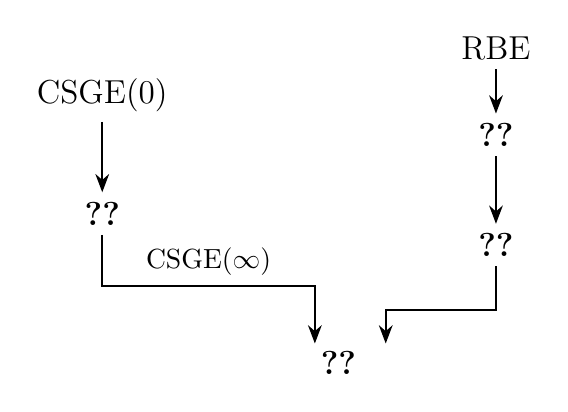
\begin{tikzpicture}[
    >=Stealth,
    every node/.style={font=\large},
    arrow/.style={->, thick},
    bracearrow/.style={thick}
]

% left branch
\node (csge) at (0,3.4) {CSGE(0)};
\node (lem46) at (0,1.9) {\cref{lem:l1_l2_talagrand}};

\draw[arrow] (csge) -- (lem46);

% right branch
\node (rbe)   at (5,4.0) {RBE};
\node (lem44) at (5,2.9) {\cref{lem:local_bobkov}};
\node (lem45) at (5,1.5) {\cref{lem:improved_talagrand}};

\draw[arrow] (rbe) -- (lem44);
\draw[arrow] (lem44) -- (lem45);

% theorem
\node (thm43) at (3.0,0) {\cref{thm:eldan_gross}};

% smoothing lemma path from Lem 4.6 to Thm 4.3
\draw[bracearrow]
    (lem46.south) -- ++(0,-0.65)
    -- node[above, midway, font=\normalsize] {CSGE($\infty$)}
    ++(2.7,0)
    -- ++(0,-0.35);

\draw[arrow] (2.7,0.9) -- (2.7,0.25);

% path from Lem 4.5 to Thm 4.3
\draw[bracearrow]
    (lem45.south) -- ++(0,-0.55)
    -- ++(-1.4,0)
    -- ++(0,-0.35);

\draw[arrow] (3.6,0.6) -- (3.6,0.25);

\end{tikzpicture}
\caption{The written lemmas and theorems. Generated by ChatGPT.}
\end{figure}

\subsection{Bobkov and Talagrand's variance-surface area inequality}
\begin{theorem}[Bobkov inequality]\label{lem:local_bobkov}
    Let $\mu$ be a distribution supported on $\Omega = \{\pm 1\}^n$ and $\{q_i: \Omega \mapsto \R_+\}_{i\in[n]}$ be transition rates reversible for $\mu$.
    Assume $\{w_i:\Omega \to \R_+\}_{i\in[n]}$ is a collection of weight functions that are $b$-bounded for some $b \in (0,1]$. 
    
    If the reinforced Bakry--\'Emery condition (equivalently, the strong gradient estimate) holds with constant $\rho > 0$,
    then, for any $f:\Omega \to [0,1]$ and $t\geq 0$, it holds
    \begin{align}\label{eq:local_bobkov}
        \+I(P_t f)\leq P_t\tp{\sqrt{\+I(f)^2 + \gamma(t) \Gamma_w(f)}},
    \end{align}
    where $\gamma(t) = \frac{2(1-e^{-2\rho t})}{b \rho}$ and $\+I:[0,1] \to \R$ denotes the Gaussian isoperimetric function.

    In particular, by taking $t \to +\infty$ on both sides, it holds
    \begin{align*}
        \+I(\E[\mu]{f}) \le \E[\mu]{\sqrt{\+I(f)^2 + \frac{2}{b \rho} \Gamma_w(f)}}.
    \end{align*}
    % \ZC{In particular, ...(add the version with $t = \infty$)
    % }
\end{theorem}

\begin{proof}
    Fix $f : \Omega \to [0,1]$ and $t \ge 0$.
    By applying the argument to $f_\varepsilon:=\varepsilon+(1-2\varepsilon)f$, where $0<\varepsilon<1/2$, and then letting $\varepsilon\downarrow0$, we may assume that $f$ takes values in $(0,1)$; in particular, $F>0$ below.
    Let $\Psi(s) = P_s \tp{\sqrt{\+I(P_{t-s} f)^2 + \gamma(s) \Gamma_w(P_{t-s} f)}}$. It suffices to prove that $\Psi$ is monotone increasing. By a standard calculation, it holds
    \begin{align}\label{eq:dPsi-1}
    \frac{\dif}{\dif s} \Psi(s) &= P_s L\tp{\sqrt{\+I(P_{t-s} f)^2 + \gamma(s) \Gamma_w(P_{t-s} f)}} + P_s \frac{\dif}{\dif s}\sqrt{\+I(P_{t-s} f)^2 + \gamma(s) \Gamma_w(P_{t-s} f)}
    \end{align}
    Let $F = \+I(P_{t-s} f)^2 + \gamma(s) \Gamma_w(P_{t-s} f)$. By chain rule, it holds
    \begin{align}\label{eq:dPsi-2}
    \frac{\dif}{\dif s} \sqrt{F} &= \frac{1}{2\sqrt{F}}\cdot\tp{- 2 \+I(P_{t-s} f) \+I'(P_{t-s} f) \cdot P_{t-s} L f + \gamma'(s) \Gamma_w(P_{t-s} f) - 2\gamma(s) \Gamma_w(P_{t-s} f, L P_{t-s} f)}
    \end{align}
    By~\Cref{lem:chain-rule}, it holds
    \begin{align}\label{eq:dPsi-3}
        2\sqrt{F} L \sqrt{F} =  L F - 2\Gamma(\sqrt{F}).
    \end{align}
    % \ZC{add a citation for \cref{eq:dPsi-3}: \Cref{lem:chain-rule}.}
    Furthermore, the reinforced Bakry--\'Emery condition reads
    \begin{align}\label{eq:dPsi-4}
        \gamma(s) L \Gamma_w(P_{t-s} f) - 2 \gamma(s) \Gamma_w(P_{t-s} f, L P_{t-s} f) - 2\rho \gamma(s) \Gamma_w(P_{t-s} f) \ge 2 \gamma(s)\Gamma\tp{\sqrt{\Gamma_w(P_{t-s} f)}}.
    \end{align}
    Combining~\eqref{eq:dPsi-1},~\eqref{eq:dPsi-2},~\eqref{eq:dPsi-3} and~\eqref{eq:dPsi-4}, it holds
    \begin{align}\label{eq:dPsi-5}
    \frac{\dif }{\dif s} \Psi(s) \ge P_s \frac{R}{2\sqrt{F}},
    \end{align}
    where
    \begin{align}\label{eq:dPsi-6}
    R = L \+I^2 (P_{t-s} f) - 2 \Gamma(\sqrt{F}) - 2 \+I(P_{t-s} f) \+I'(P_{t-s} f) P_{t-s} L f+ \frac{4}{b}\Gamma_w(P_{t-s} f) + 2\gamma(s) \Gamma(\sqrt{\Gamma_w(P_{t-s}f)})
    \end{align}
    Note that by Minkowski inequality, it holds
    \begin{align*}
        2\Gamma(\sqrt{F})(x) &= \sum_{i=1}^n q_i(x) \tp{\sqrt{\+I^2(P_{t-s} f)(x) + \gamma(s) \Gamma_w(P_{t-s} f)(x)} - \sqrt{\+I^2(P_{t-s} f)(x^i) + \gamma(s) \Gamma_w(P_{t-s} f)(x^i)}}^2\\
        &\le \sum_{i=1}^n q_i(x) \tp{\tp{\+I(P_{t-s} f)(x) - \+I(P_{t-s} f)(x^i)}^2 + \gamma(s) \tp{\sqrt{\Gamma_w(P_{t-s} f)(x)} - \sqrt{\Gamma_w(P_{t-s} f)(x^i)}}^2}\\
        &=2\Gamma(\+I(P_{t-s}f))(x) + 2\gamma(s) \Gamma(\sqrt{\Gamma_w(P_{t-s} f)})(x).
    \end{align*}
    Combining~\eqref{eq:dPsi-5} and~\eqref{eq:dPsi-6}, it only remains to show
    \begin{align}\label{eq:dPsi-7}
        L \+I^2(P_{t-s} f) - 2 \+I(P_{t-s} f) \+I'(P_{t-s} f) P_{t-s} L f+ \frac{4}{b}\Gamma_w(P_{t-s} f) - 2 \Gamma(\+I(P_{t-s} f)) \ge 0.
    \end{align}
    By definition of $L$ and $\Gamma_w$, the left-hand-side of the above inequality satisfies
    \begin{align*}
    \text{LHS of~\eqref{eq:dPsi-7}}(x) &= \sum_{i=1}^n q_i(x) \tp{\+I^2(P_{t-s} f)(x^i) - \+I^2(P_{t-s} f)(x)}\\
    &- 2 \sum_{i=1}^n q_i(x) \+I(P_{t-s} f)(x) \+I'(P_{t-s} f)(x) ((P_{t-s} f)(x^i) - P_{t-s}(f)(x))\\
    &+ \frac{2}{b}\sum_{i=1}^n q_i(x) w_i(x) \tp{P_{t-s} f(x^i) - P_{t-s} f(x)}^2\\
    &-\sum_{i=1}^n q_i(x) (\+I(P_{t-s} f)(x^i) - \+I(P_{t-s} f)(x))^2,
    \end{align*}
    which is non-negative by $w_i(x) \ge b$ and
    \begin{align*}
        \+I(x)\tp{\+I(y) - \+I(x) - \+I'(x)(y-x)} + (y-x)^2 \ge 0,
    \end{align*}
    for all $x,y \in (0,1)$.
\end{proof}

Taking $t \to \infty$ and use $\+I(x) \ge x(1-x) \sqrt{\log \frac{\e}{x(1-x)}}$ for all $x \in [0,1]$, we obtain the following improved Talagrand inequality.

\begin{corollary}[Talagrand's Variance-Surface Area inequality]\label{lem:improved_talagrand}
    Let $\mu$ be a distribution supported on $\Omega = \{\pm 1\}^n$ and $\{q_i: \Omega \mapsto \R_+\}_{i\in[n]}$ be transition rates reversible for $\mu$.
    Assume $\{w_i:\Omega \to \R_+\}_{i\in[n]}$ is a collection of weight functions that are $b$-bounded for some $b \in (0,1]$. 
    
    Suppose the following conditions hold: 
    \begin{itemize}
        \item The reinforced Bakry--\'Emery condition (equivalently, the strong gradient estimate) holds with constant $\rho_{\RBE} > 0$;
        \item The log-Sobolev inequality holds with constant $\rho_{\LSI} > 0$.
    \end{itemize}
    Then, for any $f:\Omega \to \{0,1\}$, it holds
   \begin{align}\label{eq:improved_talagrand}
        A_w(f) 
        \geq C(\rho_{\LSI},\rho_{\RBE},b) \cdot \Var[\mu]{f}\sqrt{\log \frac e{\Var[\mu]{f}}}.
   \end{align}
\end{corollary}



\subsection{Talagrand's $L^1$--$L^2$ and KKL inequality}

\begin{theorem}[Weak $L^1$--$L^2$ Talagrand inequality]\label{lem:l1_l2_talagrand_weak}
    Let $\mu$ be a distribution supported on $\Omega = \{\pm 1\}^n$ and $\{q_i: \Omega \mapsto \R_+\}_{i\in[n]}$ be transition rates reversible for $\mu$.
    Assume the strong gradient estimate~\eqref{eq:SGE} holds with constant $\rho_{\SGE} > 0$, and $\{w_i:\Omega \to \mathbb{R}_+\}_{i \in [n]}$ is a collection of weight functions that are $b$-bounded for some $b \in (0,1]$. It holds for any $f:\Omega \to \R$,
    \begin{align}\label{eq:l1_l2_talagrand_weak}
        I(f) \geq C(b,\rho_{\LSI},\rho_{\SGE})\cdot \Var[\mu]{f}\tp{1 + \log \frac{I_w(f)}{A_w(f)^2}} .
    \end{align}
\end{theorem}

\begin{proof}
Note that
\begin{align*}
\Var[\mu]{f} = 2 \int_0^{+\infty} \E[\mu]{\Gamma(P_t f)} \dif t &\le \frac{2}{b} \int_0^{+\infty} \E[\mu]{\Gamma_w(P_tf)} \dif t\\
&\le \frac{2}{b} \int_0^{+\infty} \e^{-2 \rho_{\mathrm{SGE}} t} \cdot \E[\mu]{\tp{P_t \sqrt{\Gamma_w f}}^2 } \dif t,
\end{align*}
where the last inequality follows from~\eqref{eq:SGE}. By hypercontractivity, it holds
\begin{align*}
    \E[\mu]{(P_t \sqrt{\Gamma_w f})^2} = \norm{P_t \sqrt{\Gamma_w f}}_2^2 \le \norm{\sqrt{\Gamma_w f}}^2_{p_t} \le \norm{\sqrt{\Gamma_w f}}_{1}^{2 \theta_t} \norm{\sqrt{\Gamma_w f}}_2^{2 (1-\theta_t)},
\end{align*}
where $p_t = 1 + \e^{-2\rho_{\mathrm{LSI}} t}$ and $\theta_t = \frac{2}{p_t} - 1 = \tanh (\rho_{\LSI} t)$, and the last inequality follows from H\"older's inequality.
Note that $\norm{\sqrt{\Gamma_w f}}_1 = A_w(f)$, $\norm{\sqrt{\Gamma_w f}}_2^2 = I_w(f)$. Therefore, it holds
\begin{align}\label{eq:var-bound}
    \Var[\mu]{f} \le \frac{2}{b} \int_0^{+\infty} \e^{-2 \rho_{\SGE} t} \cdot A_w(f)^{2 \theta_t} I_w(f)^{1-\theta_t} \dif t \le \frac{2 I_w(f)}{b} \int_0^{+\infty} \e^{-2 \rho_{\SGE} t} \tp{\frac{A_w(f)^2}{I_w(f)}}^{\theta_t} \dif t.
\end{align}
Let $R = \frac{I_w(f)}{A^2_w(f)} \ge 1$ and $\kappa = \min\set{\rho_{\SGE},\rho_{\LSI}}$. By $\tanh x \ge \tanh(1) \cdot \min\set{x,1}$, it holds
\begin{align*}
\int_0^{+\infty} \e^{-2 \rho_{\SGE} t} R^{-\tanh(\rho_{\LSI} t)} \dif t &\le \int_0^{+\infty} \e^{-2 \kappa t} R^{-\tanh(1) \cdot \min\set{\kappa t, 1}} \dif t\\
&\le \int_0^{\frac{1}{\kappa}} \exp\tp{- \kappa t \tp{2 + \tanh (1) \log R}} \dif t\\
&+ R^{-\tanh(1)} \cdot \int_{\frac{1}{\kappa}}^{+\infty} \exp\tp{-2\kappa t} \dif t\\
&= \frac{1-\e^{-2}R^{-\tanh(1)}}{\kappa (2+\tanh(1) \log R)} + \frac{\e^{-2} R^{-\tanh (1)}}{2 \kappa}.
\end{align*}
By $R^{-\tanh(1)} \le \frac{1}{\tanh(1)\tp{1+\log R}}$, the integral can be further bounded by $\frac{1}{C(1+\log R)}$ for some constant $C = C(\kappa) > 0$. Combining~\eqref{eq:var-bound}, it holds
\begin{align*}
\Var[\mu]{f} \lesssim \frac{I_w(f)}{1+\log \frac{I_w(f)}{A_w(f)^2}} \lesssim  \frac{I(f)}{1+\log \frac{I_w(f)}{A_w(f)^2}}.
\end{align*}
This concludes the proof.
\end{proof}

With the coordinate-wise strong gradient estimate, we establish the following $L^1-L^2$ inequality, first introduced in~\cite{CorderoErausquinLedoux12}.
% By a similar argument, we are able to establish the $L^1-L^2$ Talagrand inequality.
% \ZC{Attribute the result to \cite{CorderoErausquinLedoux12}.}
\begin{theorem}[$L^1$--$L^2$ Talagrand inequality]\label{lem:l1_l2_talagrand}
     Let $\mu$ be a distribution supported on $\Omega = \{\pm 1\}^n$ and $\{q_i: \Omega \mapsto \R_+\}_{i\in[n]}$ be transition rates reversible for $\mu$.
    Assume~\eqref{eq:0-CSGE} holds with constant $\rho_{\CSGE} > 0$, and $\{w_i:\Omega \to \mathbb{R}_+\}_{i \in [n]}$ is a collection of weight functions that are $b$-bounded for some $b \in (0,1]$. The following inequality holds for any $f:\Omega \to \R$:
    \begin{align}\label{eq:l1_l2_talagrand_2}
        \Var[\mu]{f} \leq C_1(b,\rho_{\LSI},\rho_{\CSGE}) \cdot \sum_{i=1}^n \frac{I_{w,i} (f)}{1 + \log\tp{\sqrt{I_{w,i}(f)} / \E[\mu]{|\delta_{w,i} f|}}}.
    \end{align}
    A summand is interpreted as zero when $I_{w,i}(f)=0$.
    Furthermore, we have that
    \begin{align}\label{eq:l1_l2_talagrand_3}
        I(f) \geq C_2(b,\rho_{\LSI},\rho_{\CSGE})\cdot \Var[\mu]{f}\tp{1 + \log \frac{I_w(f)}{J_w(f)}} .
    \end{align}
\end{theorem}

\begin{proof}
Similar to the previous proof, the variance $\Var[\mu]{f}$ can be bounded by
\begin{align*}
\Var[\mu]{f} \le \frac{2}{b} \int_0^{+\infty} \E[\mu]{\norm{\abs{\nabla_w} P_t f}_2^2} \dif t \le \frac{2}{b}\int_0^{+\infty} \e^{-2 \rho_{\CSGE} t}\E[\mu]{ \norm{P_t \abs{\nabla_w} f}_2^2} \dif t.
\end{align*}
Let $g_i = \abs{\delta_{w,i}} f$. It holds
\begin{align}\label{eq:var-bound-2}
\Var[\mu]{f} \le \frac{2}{b} \sum_{i=1}^n \int_0^{+\infty} \e^{- 2 \rho_{\CSGE} t} \norm{P_t g_i}_2^2 \dif t.
\end{align}
Following exactly the same argument as in the previous proof, the integral can be bounded by
\begin{align*}
\int_0^{+\infty} \e^{-2 \rho_{\CSGE} t} \norm{P_t g_i}_2^2 \dif t \le \norm{g_i}_2^2 \int_0^{+\infty}  \e^{-2 \rho_{\CSGE} t} \tp{\frac{\norm{g_i}_1^2} {\norm{g_i}_2^2}}^{\theta_t} \dif t \lesssim \frac{\norm{g_i}_2^2}{1+\log \frac{\norm{g_i}_2}{\norm{g_i}_1}} 
\end{align*}
The proof of~\eqref{eq:l1_l2_talagrand_2} then follows from~\eqref{eq:var-bound-2}, $\norm{g_i}_1 = \E[\mu]{\abs{\delta_{w,i}} f}$ and $\norm{g_i}_2 = \sqrt{I_{w,i}(f)}$.

To prove~\eqref{eq:l1_l2_talagrand_3}, we observe
\begin{align*}
    \sum_{i=1}^n \norm{P_t g_i}_2^2 \le \sum_{i=1}^n \norm{g_i}_1^{2\theta_t} \norm{g_i}_2^{2(1-\theta_t)} \le \tp{\sum_{i=1}^n \norm{g_i}_1^2}^{\theta_t} \tp{\sum_{i=1}^n \norm{g_i}_2^2}^{1-\theta_t},
\end{align*}
where $\theta_t = \tanh\tp{\rho_{\LSI} t}$ and the last inequality follows from H\"older inequality. By $J_w(f) = \sum_{i=1}^n \norm{g_i}_1^2$ and $I_w(f) = \sum_{i=1}^n \norm{g_i}_2^2$, we have
\begin{align*}
    \Var[\mu]{f} \lesssim \frac{I_w(f)}{1+\log \frac{I_w(f)}{J_w(f)}}. 
\end{align*}
This completes the proof of~\eqref{eq:l1_l2_talagrand_3}.
\end{proof}

\begin{corollary}[KKL]\label{cor:KKL}
    {\color{red} TODO}
\end{corollary}

\subsection{Eldan--Gross inequality}

\begin{theorem}[Eldan--Gross inequality]\label{thm:eldan_gross}
     Let $\mu$ be a distribution supported on $\Omega = \{\pm 1\}^n$ and $\{q_i: \Omega \mapsto \R_+\}_{i\in[n]}$ be transition rates reversible for $\mu$.
    Assume both~\eqref{eq:0-CSGE} and~\eqref{eq:infty-CSGE} holds with constant $\rho_{\CSGE} > 0$, and $\{w_i:\Omega \to \mathbb{R}_+\}_{i \in [n]}$ is a collection of weight functions that are $b$-bounded for some $b \in (0,1]$.
    For any Boolean function $f:\Omega \to \{\pm 1\}$, it holds
   \begin{align}\label{eq:eldan_gross}
        A_w(f) %\E[\mu]{\norm{\nabla_w f}_2}
        \geq C(\rho_{\LSI},\rho_{\CSGE},b) \cdot \Var[\mu]{f}\sqrt{\log\tp{1 + \frac e{J_w(f)}}}.
   \end{align}

\end{theorem}
\begin{proof}
Fix non-constant Boolean function $f:\{\pm 1\}^n \to \{\pm 1\}$. When $\Var[\mu]{f} \le \sqrt{J_w(f)}$, 
the improved Talagrand inequality (\Cref{lem:improved_talagrand}) implies the Eldan-Gross inequality: 
\begin{align*}
A_w(f) \gtrsim \Var[\mu]{f} \sqrt{\log \frac{\e}{\Var[\mu]{f}}} \gtrsim \Var[\mu]{f} \sqrt{\log \tp{1+\frac{\e}{\Var[\mu]{f}^2}}} \gtrsim \Var[\mu]{f} \sqrt{\log \tp{1+\frac{\e}{J_w(f)}}}.
\end{align*}
Therefore, we may assume $\Var[\mu]{f} \ge \sqrt{J_w(f)}$ in the following.

By Poincar\'e inequality,~\Cref{lem:l1_l2_talagrand} and~\eqref{eq:infty-CSGE}, it holds for any $s \ge 0$ that
\begin{align*}
I(P_s f) \gtrsim \Var[\mu]{P_s f} \tp{1 + \log \frac{I_w(P_s f)}{J_w(P_s f)}} \gtrsim \Var[\mu]{P_s f} \tp{1 + \log_+ \frac{\Var[\mu]{P_s f}}{J_w(f)}}.
\end{align*}

Let $T = \min\{s \ge 0 \mid \Var[\mu]{P_s f} \le \Var[\mu]{f}\}$. It holds
\begin{align*}
\frac{\Var[\mu]{f}}{2} = \Var[\mu]{f} - \Var[\mu]{P_T f} = \int_0^{T} I(P_s f) \dif s &\gtrsim \int_0^{T} \Var[\mu]{P_s f} \tp{1 + \log_+ \frac{\Var[\mu]{P_s f}}{J_w(f)}} \dif s\\
&\gtrsim  \Var[\mu]{f} \tp{1 + \log_+ \frac{\Var[\mu]{f}}{J_w(f)}} T.
\end{align*}
This implies $T \tp{1 + \log_+ \frac{\Var[\mu]{f}}{J_w(f)}} \lesssim 1$.

Let $h = \frac{1+f}{2}$. By~\Cref{lem:local_bobkov}, it holds for any $s \ge 0$ that
\begin{align*}
P_s h - (P_s h)^2 \le \+I(P_s h) \lesssim \sqrt{\gamma(s)} P_s \sqrt{\Gamma_w(h)}
\end{align*}
By taking expectation over $\mu$ on both sides, we have
\begin{align*}
\Var[\mu]{f} - \Var[\mu]{P_s f} \lesssim \sqrt{\gamma(s)} A_w(f) \lesssim \sqrt{s} A_w(f).
\end{align*}
By taking $s = T$, it holds
\begin{align*}
A_w(f) \gtrsim \frac{\Var[\mu]{f}}{\sqrt{T}} \gtrsim \Var[\mu]{f} \sqrt{1+\log_+\frac{\Var[\mu]{f}}{J_w(f)}} \gtrsim \Var[\mu]{f} \sqrt{\log \tp{1+\frac{\e}{J_w(f)}}},
\end{align*}
where the last inequality follows from the assumption $\Var[\mu]{f} \gtrsim \sqrt{J_w(f)}$.
\end{proof}


\section{Sufficient Conditions for Gradient Estimates}


In this section, we establish \ref{eq:CSGE} by choosing appropriate transition rates and weights, and the resulting bound can be controlled by norms of the Dobrushin influence matrix.

\subsection{Canonical transition rates and weights}
Given a distribution $\mu$ supported on $\Omega=\{\pm 1\}^n$, for any $x \in \Omega$ and $i \in [n]$, we define
\begin{align}\label{eq:canonical-r-w}
    q^\star_i(x) = \frac 12\sqrt{\frac{\mu(x^i)}{\mu(x)}}
        \qquad\text{and}\qquad
    w^\star_i(x) = 2q^\star_i(x) = \sqrt{\frac{\mu(x^i)}{\mu(x)}}.
\end{align}
It is straightforward to show that such transition rates $\{q^\star_i\}_{i \in [n]}$ satisfy the detailed balance condition and hence the associated heat semigroup $(P_t)_{t\ge 0}$ is reversible with respect to $\mu$.
We call \Cref{eq:canonical-r-w} the \emph{canonical transition rates and weights} associated with $\mu$. 

Under the canonical rates and weights, many notions in the $\Gamma$-calculus simplify to a nice form, which we summarize below.
Throughout, we use superscript $\star$ to indicate that the weight functions are canonical, and thereby omit $w^\star$ in the subscript; e.g., $\Gamma^\star = \Gamma_{w^\star}$ denotes the weighted carr\'e du champ operator under $q^\star$ and $w^\star$.
We have the following:
\begin{align*}
    \delta^\star_i f(x) &= \sqrt{\frac{1}{2} w^\star_i(x) q^\star_i(x)} (f(x^i) - f(x)) = q^\star_i(x) (f(x^i) - f(x)); \\
    \grad^\star f &= (\delta^\star_1 f, \dots, \delta^\star_n f); \quad
    L f = \sum_{i=1}^n \delta^\star_i f; \quad
    %\Gamma_{w,i} f(x) = q_i(x)^2 (f(x^i) - f(x))^2 \\
    \Gamma^\star f = \sum_{i=1}^n (\delta^\star_i f)^2.
\end{align*}

We also record two important properties of the canonical transition rates and weights. These properties are essential for establishing \ref{eq:SGE} and \ref{eq:CSGE}.

\begin{fact}[Square property]\label{fact:square}
    For any $i,j \in [n]$ and $x \in \Omega$, we have
    \begin{align*}
        q^\star_i(x) q^\star_j(x^i) = q^\star_j(x) q^\star_i(x^j).
    \end{align*}
\end{fact}

\begin{lemma}
\label{lem:commutator}
    Let $\mu$ be a distribution supported on $\Omega = \{\pm 1\}^n$.
    Let $M: \Omega \to \R^{n \times n}$ be a matrix field defined by, for each $x \in \Omega$,
    \begin{align}\label{eq:local-matrix}
        M_{ij}(x) := 
        \begin{cases}
            \frac{1}2 \tp{\sqrt{\frac{\mu(x^{ij})}{\mu(x^i)}}-\sqrt{\frac{\mu(x^j)}{\mu(x)}}}, & i \neq j;\\
            0, & i = j.
        \end{cases}
    \end{align}
    For any function $f: \Omega \to \R$,
    \begin{align*}
        (L \grad^\star - \grad^\star L) f = \left( \diag\{M\*1\} - M^\top \right) \grad^\star f.
    \end{align*}
\end{lemma}

\begin{proof}
    % \ZC{@Zejia: You need to make the proof more comprehensible. For example, for this proof, first calculate $\delta^\star_j \delta^\star_i - \delta^\star_i \delta^\star_j$, then $L \delta^\star_i - \delta^\star_i L$, and finally $L \grad^\star - \grad^\star L$ (the latter two should follow straightforwardly). Use
    % \begin{align*}
    %     \grad^\star f &= (\delta^\star_1 f, \dots, \delta^\star_n f);\\
    %     L f &= \sum_{i=1}^n \delta^\star_i f;
    % \end{align*}
    % which were mentioned above, to simplify the presentation (doesn't mean shorter proof, but easier to understand). Your proof should rely on the square property, and you should explicitly mention it; this helps the reader understand why the canonical rates and weights work.}
    
    
    Fix $f: \Omega\mapsto \R$, $x\in \Omega$.
    For any $i,j \in [n]$ with $i\neq j$, by definition,
    $$
        \delta^\star_j \delta^\star_i f(x) = q^\star_j(x) (\delta^\star_i f(x^j) - \delta^\star_i f(x)) = q^\star_j(x) q^\star_i(x^j)(f(x^{ij})-f(x^j)) - q^\star_j(x)q^\star_i(x)(f(x^i)-f(x)).
    $$
    \Cref{fact:square} implies that the cancellation of the second derivative in the commutator term $\delta^\star_i\delta^\star_j - \delta^\star_j\delta^\star_i$. 
    We have that,
    \begin{align}
        (\delta^\star_j \delta^\star_i - \delta^\star_i \delta^\star_j) f(x) &= (q_j^\star(x)q_i^\star(x^j) - q_i^\star(x)q_j^\star(x^i)) f(x^{ij})  \nonumber
        \\&-(q_i^\star(x^j) - q_i^\star(x))q_j^\star(x)f(x^j)+(q_j^\star(x^i) - q_j^\star(x))q_i^\star(x)f(x^i) \nonumber
        \\&= M_{ij}(x)q_i^\star(x)f(x^i) - M_{ji}(x)q_j^\star(x)f(x^j), \nonumber
        \\&= M_{ij}(x)\delta^\star_i f(x) - M_{ji}(x)\delta^\star_j f(x), \label{eq:commutator_delta_ij}
    \end{align}
    where the last equality follows from $M_{ij}(x) q_i^\star(x) = M_{ji}(x) q_j^\star(x)$ by \Cref{fact:square}.
    Then the following equality immediately follows from
    \Cref{eq:commutator_delta_ij},
    \begin{align}
        (L\delta^\star_i - \delta^\star_iL) f(x) &= (\sum_{j=1}^n \delta^\star_j\delta^\star_i - \delta^\star_i\delta^\star_j)f(x)
        = \sum_{j=1}^n M_{ij}(x)\delta^\star_i f(x) - \sum_{j=1}^n M_{ji}(x)\delta^\star_j f(x) \nonumber
        \\&= \tp{M(x)\*1}_i\delta^\star_i f(x) - \inner{(M^\top(x))_i}{\nabla^\star f(x)}, \nonumber
    \end{align}
    that is, $(L \grad^\star - \grad^\star L) f = \left( \diag\{M\*1\} - M^\top \right) \grad^\star f$ holds for any $x\in \Omega$.
\end{proof}




\subsection{Sufficient condition for SGE} \label{sec:SGE_boolean_hypercube}

\begin{theorem}[SGE under canonical transition rates and weights]
\label{thm:SGE_boolean_hypercube}
    Let $\mu$ be a distribution on $\Omega = \{\pm 1\}^n$ with full support. Let $M,D: \Omega \to \R^{n \times n}$ be two matrix fields where $M$ is defined by \Cref{eq:local-matrix} and $D$ is defined by, for each $x \in \Omega$,
    \begin{align}\label{eq:def-D}
        D(x) := \diag\left\{\sqrt{\frac{\mu(x)}{\mu(x^i)}}\right\}_{i\in[n]}.
    \end{align}
    Then, under the canonical transition rates and weights, \ref{eq:SGE} holds with constant
    \begin{align*}
        \rho = \min_{x \in \Omega} \;
        \lambda_{\min}\left( D(x) + \diag\{M(x)\*1\} - \frac{1}{2}\left( M(x) + M(x)^\top \right) \right),
    \end{align*}
    where $\lambda_{\min}(A)$ denotes the minimum eigenvalue of a symmetric matrix $A$.
\end{theorem}

\begin{proof}
    By \Cref{prop:equivalence_BE_GE}, it is sufficient to establish the \ref{eq:rBE} condition.
    Specifically, for any function $f: \Omega \to \R$, we aim to show the following pointwise inequality:
    \begin{align*}
        \Gamma^\star_2(f) - \Gamma(\sqrt{\Gamma^\star(f)}) \ge \rho \cdot \Gamma^\star(f),
    \end{align*}
    where we recall that $\Gamma$ is the unweighted carr\'e du champ operator with respect to the canonical rates $q^\star$.
    By \Cref{lem:gamma2-formula}, we have
    \begin{align}
        \Gamma^\star_2(f) - \Gamma(\sqrt{\Gamma^\star(f)}) 
        = \sqrt{\Gamma^\star(f)} L \sqrt{\Gamma^\star(f)} - \Gamma^\star(f,Lf) 
        = \norm{\nabla^\star f}_2 L \norm{\nabla^\star f}_2 - \inner{\nabla^\star f}{\nabla^\star Lf}. \label{eq:first-rBE}
        %&= \tp{ \norm{\nabla^\star f}_2 L \norm{\nabla^\star f}_2 - \inner{\nabla^\star f}{L \nabla^\star f} } + \inner{\nabla^\star f}{(L \nabla^\star - \nabla^\star L) f}.
    \end{align}

    
    Fix $x\in \Omega$. For the first term, we have that
    \begin{align}
        \norm{\nabla^\star f}_2 L \norm{\nabla^\star f}_2 (x)
        &= \norm{\nabla^\star f(x)}_2 \sum_{i=1}^n q^\star_i(x) \tp{\norm{\nabla^\star f(x^i)}_2 - \norm{\nabla^\star f(x)}_2} \nonumber \\
        &= \sum_{i=1}^n q^\star_i(x) \tp{\norm{\nabla^\star f(x)}_2 \norm{\nabla^\star f(x^i)}_2 - \norm{\nabla^\star f(x)}_2^2}. \label{eq:norm-L-norm}
    \end{align}
    We then deduce from the Cauchy--Schwarz inequality that
    \begin{align}
        \norm{\nabla^\star f(x)}_2 \norm{\nabla^\star f(x^i)}_2
        &\ge \inner{\nabla^\star f(x)}{\nabla^\star f(x^i)} + 2|\delta^\star_i f(x)| |\delta^\star_i f(x^i)| \nonumber\\
        &= \inner{\nabla^\star f(x)}{\nabla^\star f(x^i)} + 2 \frac{q^\star_i(x^i)}{q^\star_i(x)} (\delta^\star_i f(x))^2. \label{eq:cauchy-schwarz}
    \end{align}
    where we crucially use the fact that $\delta^\star_i f(x) = q^\star_i(x) (f(x^i)-f(x))$ and $\delta^\star_i f(x^i) = q^\star_i(x^i) (f(x)-f(x^i))$ have opposite sign.
    Combining \Cref{eq:norm-L-norm,eq:cauchy-schwarz},
    \begin{align*}
        \norm{\nabla^\star f}_2 L \norm{\nabla^\star f}_2 (x)
        &\ge \sum_{i=1}^n q^\star_i(x) \tp{ \inner{\nabla^\star f(x)}{\nabla^\star f(x^i)} + 2 \frac{q^\star_i(x^i)}{q^\star_i(x)} (\delta^\star_i f(x))^2 - \inner{\nabla^\star f(x)}{\nabla^\star f(x)} } \\
        &= \sum_{i=1}^n 2 q^\star_i(x^i) (\delta^\star_i f(x))^2 + \sum_{i=1}^n q^\star_i(x) \inner{\nabla^\star f(x)}{\nabla^\star f(x^i) - \nabla^\star f(x)} \\
        &= \inner{\grad^\star f}{D \grad^\star f} (x) + \inner{\nabla^\star f}{L \nabla^\star f} (x).
    \end{align*}
    Plugging into \Cref{eq:first-rBE} and combining \Cref{lem:commutator}, we deduce
    \begin{align*}
        \Gamma^\star_2(f) - \Gamma(\sqrt{\Gamma^\star(f)}) 
        &\ge \inner{\grad^\star f}{D \grad^\star f} + \inner{\nabla^\star f}{(L \nabla^\star - \nabla^\star L) f} \\
        &= \inner{\grad^\star f}{\left( D + \diag\{M\*1\} - M^\top \right) \grad^\star f}
        \ge \rho \norm{\grad^\star f}_2^2 = \rho \cdot \Gamma^\star(f),
    \end{align*}
    where the last inequality holds for any constant $\rho \le \lambda_{\min} \left( D + \diag\{M\*1\} - \frac{1}{2}(M+M^\top) \right)$ uniformly at all points $x \in \Omega$.
\end{proof}

\subsection{Sufficient condition for CSGE} 
\label{sec:CSGE_boolean_hypercube}

\begin{theorem}[CSGE under canonical transition rates and weights]
\label{thm:CSGE_boolean_hypercube_w=q}
    Let $\mu$ be a distribution on $\Omega = \{\pm 1\}^n$ with full support. Let $M,D: \Omega \to \R^{n \times n}$ be two matrix fields defined by \Cref{eq:local-matrix,eq:def-D}, respectively. Let $M^\star := (\sup_x|M_{ij}(x)|)_{i,j \in [n]}$ and $D^\star = (\inf_x D_{ij}(x))_{i,j \in [n]}$ denote the entrywise uniform upper and lower bound on $\abs{M}$ and $D$, respectively. 
    Then, under the canonical transition rates and weights, for any $\tau \in \R_+$, \ref{eq:CSGE} holds with constant
    \begin{align*}
        \rho =
        \lambda_{\min}\left( D^\star - \diag\{M^\star\*1\} - \frac{1}{2}\left( M^\star + (M^\star)^\top \right) \right),
    \end{align*}
    where $\lambda_{\min}(A)$ denotes the minimum eigenvalue of a symmetric matrix $A$.
\end{theorem}

\ZC{How to deal with that $F_s$ is not differentiable at $s$?}

\ZJ{Does the following idea work?

$F_s$ is not differentiable at $s$ implies that there exists $i\in [n], x\in \Omega$, $\delta_i^\star P_{t-s}f(x) = 0$?
Fix $i$ and $x$, let $g(s) = P_{t-s}f(x)$.
% Since $g$ is in $C^\infty$ and $g_s(x) = \sum_{k=0}^\infty \frac{(t-s)^k}{k!}(L^k f)(x)$ converges, $g$ is an analytic function.
For any $s,s_0\in [0,t]$, $g(s) = \sum_{i=0}^{\infty} \frac{(L^i P_{t-s_0} f(x))}{i!} (s_0-s)^i$ converges.
Therefore, $g$ is an analytic function. (?)
Then $s\mapsto \delta_i^\star P_{t-s}f(x)$ is also an analytic function.
There are finitely many zeros for an analytic function $h$ in a closed interval unless $h\equiv 0$.
Therefore, $F_s$ is differentiable almost everywhere.
}

\begin{proof}
    Fix an arbitrary function $f: \Omega \to \R$ and real numbers $\tau, t \ge 0$.
    Our goal is to show \ref{eq:CSGE} under the canonical rates and weights, namely, 
    \begin{align}\label{eq:goal-CSGE}
        \norm{P_\tau \abs{\nabla^\star}P_t f}_2 \leq e^{-\rho t} \norm{P_{\tau+t} \abs{\nabla^\star}f}_2. 
    \end{align}
    Define $F_s = e^{-2\rho s} \norm{P_{\tau+s}\abs{\nabla^\star} P_{t-s} f}_2^2$; hence, \Cref{eq:goal-CSGE} is equivalent to $F_0 \le F_t$.
    It is sufficient to show that $\frac d{ds} F_s \geq 0$ for all $s \in [0,t]$.
    
    Fix $s \in [0,t]$. To ease the notation, let $g = P_{t-s} f$.
    Taking the derivative of $F_s$ gives 
    \begin{align}
        \frac d{ds} F_s &= 2 e^{-2\rho s} \left( - \rho \norm{P_{\tau+s} |\grad^\star| g}_2^2 
        + \inner{P_{\tau+s} |\grad^\star| g}{\frac{d}{ds} P_{\tau+s} |\grad^\star| g}
        \right).
        %\\&=2e^{-2\rho s}\inner{P_{\tau+s} |\grad^\star| g}{P_{\tau+s}\left(-\rho |\grad^\star| g + L |\grad^\star| g - \sgn(\grad^\star g)\otimes \grad^\star Lg\right)}.
        \label{eq:CSGE_potential_function_derivative}
    \end{align}
    Since $P_{\tau+s} = e^{(\tau+s)L}$ and $g = P_{t-s} f = e^{(t-s)L} f$, we have that
    \begin{align}
    \label{eq:derivative-CSGE}
        \frac d{ds} P_{\tau+s} |\grad^\star| g
        &= P_{\tau+s} \left( L + \frac{d}{ds} \right) |\grad^\star| g 
        = P_{\tau+s} \left( L |\grad^\star| - \sgn(\grad^\star g) \odot \grad^\star L \right) g,
    \end{align}
    where $\sgn(\cdot)$ denotes the entrywise absolute value of a vector, and $\odot$ denotes the entrywise product of two vectors.
    To calculate this, we need an adapted version of \Cref{lem:commutator}, which is stated below and proved afterward.

    \begin{lemma}
    \label{lem:abs-commutator}
        Let $\mu$ be a distribution supported on $\Omega = \{\pm 1\}^n$.
        Let $M,D: \Omega \to \R^{n \times n}$ be two matrix fields defined by \Cref{eq:local-matrix,eq:def-D}, respectively, and let $|M| := (|M_{ij}|)_{i,j \in [n]}$ be the entrywise absolute value of $M$.
        For any function $g: \Omega \to \R$, it holds
        \begin{align*}
            \left( L |\grad^\star| - \sgn(\grad^\star g) \odot \grad^\star L \right) g \ge \left( D + \diag\{M\*1\} - |M|^\top \right) |\grad^\star| g.
        \end{align*}
        % \ZC{I got
        % \begin{align*}
        %     \left( L |\grad^\star| - \sgn(\grad^\star g) \odot \grad^\star L \right) g \ge \left( D + \diag\{M\*1\} - |M|^\top \right) |\grad^\star| g,
        % \end{align*}
        % }
        % \ZJ{We can use this tighter version, although I don't think it can improve the final conclusion.} \ZC{Agree!}
    \end{lemma}
    
    Combining \Cref{eq:derivative-CSGE,lem:abs-commutator}, 
    we deduce that
    \begin{align*}
        \inner{P_{\tau+s} |\grad^\star| g}{\frac{d}{ds} P_{\tau+s} |\grad^\star| g}
        &\geq \inner{P_{\tau+s} |\grad^\star| g}{P_{\tau+s} \left( D + \diag\{M\*1\} - |M|^\top \right) |\grad^\star| g}
        \\&\geq \inner{P_{\tau+s} |\grad^\star| g}{ \left( D^\star - \diag\{M^\star\*1\} -( M^\star)^\top \right) P_{\tau+s}|\grad^\star| g}.
    \end{align*}
    % \ZC{
    % Call $A := D + \diag\{M\*1\} - |M|^\top$, which is a matrix field $A: \Omega \to \R^{n \times n}$.
    % It is an operator acting on a vector field $v: \Omega \to \R^n$ via pointwise product:
    % \begin{align*}
    %     (Av)(x) := A(x) v(x), \quad\forall x \in \Omega.
    % \end{align*}
    % Meanwhile, $P_{\tau+s}$ is another operator acting on vector fields entrywisely:
    % \begin{align*}
    %     P_{\tau+s} v := (P_{\tau+s} v_1, \dots, P_{\tau+s} v_n).
    % \end{align*}
    % Your proof seems to claim they commute:
    % \begin{align*}
    %     P_{\tau+s} A v = A P_{\tau+s} v.
    % \end{align*}
    % Do you have a proof? This feels suspicious.\\
    % A possible fix is to define $A$ uniformly:
    % \begin{align*}
    %     A_{ij} := 
    %     \begin{cases}
    %         \min_{x \in \Omega} D_{ii}(x) + \sum_{j=1}^n M_{ij}(x), & i = j \\
    %         - \max_{x \in \Omega} |M_{ji}(x)|, & i \neq j 
    %     \end{cases}
    % \end{align*}
    % I would keep the statement in \Cref{lem:abs-commutator} the same except adding
    % \begin{align*}
    %         \left( L |\grad^\star| - \sgn(\grad^\star g) \odot \grad^\star L \right) g 
    %         \ge \left( D + \diag\{M\*1\} - |M|^\top \right) |\grad^\star| g 
    %         \ge A |\grad^\star| g.
    %     \end{align*}
    % }
    We conclude that 
    $$
        \frac{d}{ds}F_s \geq \tp{P_{\tau+s} |\grad^\star| g}^\top\tp{D^\star - \diag\{M^\star\*1\}-\frac{1}{2}(M^\star+(M^\star)^\top) - \rho I}\tp{P_{\tau+s} |\grad^\star| g} .
    $$
    Therefore, the coordinate-wise strong gradient estimate (\ref{eq:CSGE}) holds with constant $\rho = \lambda_{\min}(D^\star-\diag\{M^\star\*1\} - \frac{1}{2}(M^\star+(M^\star)^\top))$ at all $x \in \Omega$.
\end{proof}

\begin{proof}[Proof of \Cref{lem:abs-commutator}]
    % \ZC{Update the proof.}
    Define $H_{ij}(x) = \frac{q_i(x^j)}{q_i(x)}$.
    By \Cref{fact:square}, we have that $H_{ij}(x) = \frac{q_i(x^j)}{q_i(x)} = \frac{q_j(x^i)}{q_j(x)} = H_{ji}(x)$.
    For notational convenience, we occasionally omit the dependence on $x$, writing, for example, $q_i^\star$ instead of $q_i^\star(x)$.
    For $i,j\in[n]$ with $i\neq j$, the following is deduced from $H_{ij}=H_{ji}$:
    \begin{align}
        (\delta_j^\star \abs{\delta_i^\star} - \sgn(\delta^\star_i g(x))\delta_i^\star \delta_j^\star) g(x)
        &=  q_j^\star q_i^\star\tp{H_{ij}\abs{g(x^{ij}) - g(x^j)} - \abs{g(x^i) - g(x)}} \nonumber
        \\&- \sgn(\delta^\star_i g) q_i^\star q_j^\star(H_{ji}(g(x^{ij})-g(x^i)) - g(x^j)+g(x))\nonumber
        \\&=q_i^\star q_j^\star H_{ij}\tp{\abs{g(x^{ij}) - g(x^j)} - \sgn(\delta^\star_i g)(g(x^{ij}) - g(x^j))} \label{eq:abs-commutator_second_term}
        \\&+q_i^\star q_j^\star\tp{-\frac{\abs{\delta^\star_i} g}{q_i^\star} - \sgn(\delta^\star_i g)\tp{H_{ij}(g(x^j) - g(x^i)) - \frac{\delta^\star_jg}{q_j^\star}}}. \label{eq:abs-commutator_eq}
    \end{align}
    Since $\abs{a}-\sgn(b)a \geq 0$ holds for any $a,b\in\R$, \Cref{eq:abs-commutator_second_term} is non-negative, resulting in the callcelation of the second derivative term in the commutator.
    Therefore, by \Cref{eq:abs-commutator_eq}, 
    \begin{align}
        (\delta_j^\star \abs{\delta_i^\star} - \sgn(\delta^\star_i g(x))\delta_i^\star \delta_j^\star) g(x)
        &\geq - q_j^\star\abs{\delta^\star_i g} - \sgn(\delta^\star_i g)\tp{H_{ij}q_i^\star q_j^\star(\frac{\delta_j^\star g}{q_j^\star} - \frac{\delta_i^\star g}{q_i^\star}) - q_i^\star\delta^\star_jg} \nonumber
        \\&= (H_{ij} - 1)q_j^\star\abs{\delta^\star_i}g - \sgn(\delta^\star_i g) \tp{H_{ij} - 1}q_i^\star\delta^\star_j g \nonumber
        \\&\geq (H_{ij} - 1)q_j^\star\abs{\delta^\star_i}g - \abs{H_{ji} - 1}q_i^\star\abs{\delta^\star_j}g \label{eq:CSGE_commutator_term}
    \end{align}
    For the non-commutator term, we have that
    \begin{align} \label{eq:CSGE_non-commutator_term}
        (\delta_i^\star \abs{\delta_i^\star} - \sgn(\delta^\star_i g(x))\delta_i^\star \delta_i^\star)g(x) &= q_i^\star(x) \tp{\abs{\delta_i^\star}g(x^i) - \sgn(\delta^\star_i g(x))\delta_i^\star g(x^i)} \nonumber
        \\&= 2 q_i^\star(x) \abs{\delta_i^\star}g(x^i)
        = 2 q_i^\star(x^i) \abs{\delta_i^\star}g(x)
        = \frac 1{2q_i^\star(x)} \abs{\delta_i^\star}g(x),
    \end{align}
    where we use the fact that for any $i\in[n]$, $x^{ii} = x$ and $\sgn(\delta^\star_i g(x)) = \sgn(g(x^i) - g(x)) = - \sgn(g(x) - g(x^i)) = -\sgn(\delta^\star_i g(x^i))$.
    Combine \Cref{eq:CSGE_commutator_term,eq:CSGE_non-commutator_term} together, we conclude the following inequality,
    \begin{align*}
        (L\abs{\delta_i^\star} - \sgn(\delta^\star_i g(x))\delta_i^\star L) g(x) &\geq \frac{1}{2q_i^\star}\abs{\delta^\star_i} g + \sum_{j\neq i} (H_{ij} - 1)q_j^\star\abs{\delta^\star_i} g - \abs{H_{ji} - 1}q_i^\star\abs{\delta^\star_j} g
        \\&= (D_{ii} + (M_i)^\top \*1)\abs{\delta^\star_i} g - \inner{(\abs{M}^\top)_i}{\abs{\nabla^\star} g}, 
    \end{align*}
    where the last equality follows from $\abs{H_{ij}-1}p_j^\star = \abs{M_{ij}}$.
    This is exactly
    \[
        \left( L |\grad^\star| - \sgn(\grad^\star g) \odot \grad^\star L \right) g \ge \left( D + \diag\{M\*1\} - |M|^\top \right) |\grad^\star| g. \qedhere
    \]
\end{proof}


\subsection{Dobrushin condition}
In this section, we state our isoperimetric inequalities under the conditions of the Dobrushin matrix and marginal bounds. 
In addition to the CSGE condition that we establish in the above, we also require that hypercontractivity holds from \Cref{sec:boolean}.

It turns out that the largest eigenvalue of $D$ and $M$ can be controlled by suitable norms of Dobrushin influence matrix with some additional bounds associated with the canonical transition rates.
Consequently, a general and easy way to check the CSGE condition is to establish an upper bound the norms of the Dobrushin matrix and check the marginal bounds of the distribution $\mu$.
The following is the definition of the Dobrushin matrix.
\begin{definition}[Dobrushin influence]
    For finite space $\+X$, the Dobruhsin influence matrix of distribution $\mu$ over $\+X^n$ is defined as follows,
    \begin{align}\label{eq:def_Dobrushin_matrix}
        R = (R_{ij})_{i,j\in[n]},\quad R_{ij} = \sup_{x,y,x_{-j}=y_{-j}}\TV{\mu_i(\cdot\mid x_{-i})}{\mu_i(\cdot\mid y_{-i})} .
    \end{align}
    We say a distribution satisfies the Dobrushin condition if $\norm{R(\mu)}_2 < 1$.
    \ZC{Are we defining $R$ in the wrong way? $R \gets R^\top$}
    \ZJ{I saw different definitions, the current definition is the same as the definition from Frederic's \href{chrome-extension://efaidnbmnnnibpcajpcglclefindmkaj/https://frkoehle.github.io/stat31512-s2024/lecture10.pdf}{lecture notes}.}
\end{definition}

\begin{lemma}[]\label{lem:Dobrushin_upper_bound_CSGE}
     If $w_i^\star(x) \in [b,1/b]$ for any $x\in \{\pm 1\}^n$ and $i\in[n]$, then under the canonical transition rates and weights, \ref{eq:CSGE} holds with constant $\rho = b - \frac{(1+b^2)^2}{4b^3}(\norm{R}_2 + \norm{R}_1)$.
\end{lemma}
\begin{proof}
    The entries of the Dobrushin influence matrix can be expressed in terms of the canonical transition rates as follows:
    $$
        R_{ij} = \begin{cases}
            \sup_x \frac{4\abs{q_i^\star(x^j)^2-q_i^\star(x)^2}}{(1+4q_i^\star(x)^2)(1 + 4q_i^\star(x^j)^2)} &, i\neq j
            \\ 0 &, i = j
        \end{cases} .
    $$
    Then the Dobrushin matrix give an entry-wise upper bound of $M^\star = (\sup_x \abs{M_{ij}(x)})_{i,j\in[n]}$.
    That is, for any $i, j\in[n]$ and $i\neq j$,
    \begin{align}\label{eq:Dobrushin_to_CSGE_constant}
        R_{ij} \geq \tp{\inf_{u,v\in [b,1/b]}\frac{u+v}{(1+u^2)(1+v^2)}}\sup_{x\in \Omega}2\abs{q_i^\star(x)-q_i^\star(x^j)} \geq \frac{4b^3}{(1+b^2)^2}M^\star_{ji} .
    \end{align}
    % \ZC{Our goal is to show: 
    % \begin{align}
    %     A - \diag\{B\*1\}-\rho I- \frac{B+B^{\top}}{2}\succeq 0.
    % \end{align}
    % Why do we need $K$?
    % I think we have 
    % \begin{align}
    %     A \succeq c_1 I, \quad \diag\{B\*1\} \preceq c_2 I, \quad B+B^{\top} \preceq c_3 \lambda_{\max}(D+D^\top) \cdot I.
    % \end{align}
    % }
    Since $D^\star_{ii} = \inf_x w_i(x^i)$ for $i\in[n]$, $D^\star\geq_{\-{ew}} bI$.
    Therefore, by symmetry of matrices and \Cref{eq:Dobrushin_to_CSGE_constant}, we have that
    \begin{align*}
        \lambda_{\min}(D^\star-\diag\{M^\star\*1\}-\frac{1}{2}(M^\star+(M^\star)^\top)) &\geq \lambda_{\min}(D^\star) - \lambda_{\max}(\diag\{M^\star\*1\}) - \lambda_{\max}(\frac{1}{2}(M^\star+(M^\star)^\top)) 
        \\&\geq b - \frac{(1+b^2)^2}{4b^3}(\norm{R}_2 + \norm{R}_1)  \geq \rho.
    \end{align*}
    By \Cref{thm:CSGE_boolean_hypercube_w=q}, we complete the proof.
\end{proof}

The following theorem shows that for the discrete product space, the Dobrushin condition and the one-site conditional marginal lower bound are sufficient to derive \ref{eq:LSI} constant and hypercontractivity. 
\begin{theorem}[{\cite[Theorem 1.14 and Corollary 1.11]{marton2019logarithmic}}]\label{thm:marton_Dobrushin_to_LSI}
Let $\+X$ be a finite space.
Suppose the distribution $\mu$ on $\Omega = \+X^n$ satisfies the Dobrushin condition $\norm{R}_2 < 1$ and the one-site conditional marginal lower bound $\alpha = \inf_x \mu(x_i\mid x_{-i})$, then for Gibbs sampler $G = \frac 1 n\sum_{i=1}^n K_i$ where $K_i(z\mid y) = \ind[z_{-i}=y_{-i}]\mu(z_i\mid z_{-i})$, the log-Sobolev inequality holds as follows,
$$
    \forall f\in \R^\Omega, \frac 1n\Ent[\mu]{f^2} \leq \frac{2}{\alpha(1-\norm{R}_2)^2} \inner{f}{(I-G)f}_{\mu} .
$$
\end{theorem}
\begin{corollary}\label{cor:Dobrushin_to_LSI}
    Suppose $w_i^\star(x)\in [b,1/b]$ for any $x\in \{\pm 1\}^n$ and $i\in[n]$, then \ref{eq:LSI} holds with constant $\frac{b^2(1 - \norm{R}_2)^2}{1+b^2}$ with respect to the canonical transition rates $q^\star$.
\end{corollary}
\begin{proof}
    This immediately follows from
    \[
        \inner{f}{(I-G)f}_{\mu} = \E[\mu]{\frac 12\sum_{i=1}^n \frac{2q_i^\star(x)}{n(1/w_i^\star(x)+w_i^\star(x))}(f(x^i)-f(x))^2}
        \leq \frac 1n\E[\mu]{\Gamma(f,f)} . \qedhere
    \]
\end{proof}
By \Cref{thm:CSGE_boolean_hypercube_w=q}, \Cref{cor:Dobrushin_to_LSI} and \cref{sec:boolean}, we conclude the following theorem about isoperimetric inequalities.
\begin{theorem}\label{thm:Dobrushin_to_isoperimetric}
    Let $\mu$ be a distribution on $\{\pm 1\}^n$ with full support.
    Let the transition rates and weights to be the canonical ones defined in \Cref{eq:canonical-r-w}.
    Suppose that for any $x\in \{\pm 1\}^n$ and $i\in[n]$, $w_i^\star(x)\in [b,1/b]$ and $\max\{\norm{R}_1,\norm{R}_2\}\leq C$ for some constants $b,C$, where $R$ is the Dobrushin influence matrix defined in \Cref{eq:def_Dobrushin_matrix}.
    Then the local Bobkov inequality \eqref{eq:local_bobkov} holds.

    Furthermore, if the Dobrushin condition holds, the $L^1$--$L^2$ Talagrand inequality \eqref{eq:l1_l2_talagrand_2}, the KKL inequality \eqref{eq:} and the Eldan-Gross inequality \eqref{eq:eldan_gross} holds with constant depending on $\norm{R}_1$, $\norm{R}_2$ and $b$.
\end{theorem}
\subsection{Application to Ising model}
A distribution $\mu$ over $\{\pm 1\}^n$ is called an \emph{Ising model} with interaction matrix $J \in \R^{n\times n}$ and external field $h\in \R^n$ if 
$$
    \forall x\in \{\pm 1\}^n, \mu(x) \propto \exp(\frac 12 x^\top J x + h^\top x),
$$
where $J$ is a symmetric matrix.
Note that the diagonals of $J$ do not affect the distribution, hence we can assume that $J_{ii} = 0$ for $i\in[n]$.
\ZJ{previous results.}

In the following theorem, we establish a new criterion for high temperature Ising model to prove the isoperimetric inequalities under a Dobrushin-type condition by \cref{thm:Dobrushin_to_isoperimetric}.
\begin{theorem}\label{thm:Ising}
    Suppose that $\mu$ is an Ising model parameterized by zero external field $h = \*0$ and interaction matrix $J$ satisfying $\norm{J}_2 < 1$ and $\norm{J}_1\leq C$ for some constant $C > 0$.
    Let the transition rates and weights to be the canonical ones defined in \Cref{eq:canonical-r-w}.
    Then the local Bobkov inequality \eqref{eq:local_bobkov}, the $L^1$--$L^2$ Talagrand inequality \eqref{eq:l1_l2_talagrand_2}, the KKL inequality \eqref{eq:} and the Eldan-Gross inequality \eqref{eq:eldan_gross} holds with constant depending on $\norm{J}_2$ and $C$.
\end{theorem}


\begin{proof}
    Let $b = e^{-\norm{J}_1}$.
    For any $i,x$, $w_i^\star(x) = \exp(-x_iJ_i^\top x) \in [b,1/b]$.
    Fix $x\in \Omega$ and $i,j\in [n]$ with $i\neq j$.
    Define $\alpha = \sum_{k\neq i,j}J_{ik} x_k$ and $\beta = \abs{J_{ij}}$ .
    We have that 
    \begin{align*}
        \TV{\mu_i(\cdot\mid x)}{\mu_i(\cdot\mid x^j)} &= \abs{\mu(x_i=+1\mid x_j=+1,x_{-i,j}) - \mu(x_i=+1\mid x_j=-1,x_{-i,j})}
        \\&= \frac 12\abs{\tanh(\alpha+\beta) - \tanh(\alpha-\beta)}
        = \frac{2\abs{\sinh(\beta)\cosh(\beta)}}{\cosh(2\alpha)+\cosh(2\beta)}
        \\&\leq \frac{2\abs{\sinh(\beta)\cosh(\beta)}}{1+\cosh(2\beta)} = \tanh(\beta) \leq \beta.
    \end{align*}
    Therefore, $R \leq_{\-{ew}} \abs{J}$ and $\norm{R}_2\leq \norm{\abs{J}}_2 < 1$.
    We have that $\norm{J}_2 \leq \sqrt{\norm{J}_1\norm{J}_{\infty}} = \norm{J}_1$ follows from symmetry. 
    By \cref{thm:Dobrushin_to_isoperimetric}, since $\max\{\norm{R}_1,\norm{R}_2\}\leq \norm{J}_1 \leq C$, all the isopermetric inequalities in \cref{sec:boolean} hold.
\end{proof}




\section{Extension to Schreier Graphs}
In this section, we extend the framework from the Boolean hypercube $\Omega=\{\pm 1\}^n$ to Schreier graphs. This more general setting was also considered in~\cite{ODonnellWimmer13,ODonnellWimmerSharp13,CorderoErausquinLedoux12}, which established a KKL theorem for Schreier graphs given a log-Sobolev constant. Here, we derive an Eldan--Gross inequality in this setting under a slightly stronger assumption.

\subsection{Basic definitions}
Let $G$ be a group acting on a finite set $X$, and $U$ be a generating set for $G$ that is symmetric, i.e., $U^{-1} = U$. The \emph{Schreier graph} $\Sch(G,X,U)$ is a graph with vertex set $V = X$ and edge set $E = \{(x,gx) \mid x \in X, g \in U\}$. Suppose that $U = \bigcup_{i=1}^n U_i$ where each $U_i$ is symmetric, i.e., $U_i^{-1} = U_i$. We remark that $\{U_i\}$ is not necessarily a partition of $U$. {\color{red} Though, each group element $u \in U$ will appears exactly in $r$ subsets $U_i$ for some $r \ge 1$.}

Schreier graphs encompass a broad range of discrete structures, including product spaces such as $[q]^d$ and slices of the Boolean hypercube such as $\binom{[n]}{k}$.
\begin{example}\label{example:SGraph}
    Let $G = X = \Z_m^n$ and $U_i = \{k e_i: k \in [m-1]\}$. The Schreier graph $\Sch(G,X,U)$ is a Hamming graph.
\end{example}

\begin{example}
    Let $G = S_n$, $X = \binom{[n]}{k}$ and $U_i = \{(ij) \mid j \in [n] \setminus \{i\}\}$. The Schreier graph $\Sch(G,X,U)$ is the exchange graph on the Boolean slice $\binom{[n]}{k}$, and the corresponding random walk is the standard exchange walk.
\end{example}

Similar to the Boolean hypercube case, we define the carr\'e du champ operators, and influences as well as surface area of Boolean functions for the Schreier graphs.

\begin{definition}[$\Gamma$-calculus]
Let $\Sch(G,X,U)$ be a Schreier graph with $U = \bigcup_{i=1}^n U_i$. Given the transition rates $\{q_u: \Omega \to \mathbb{R}_{+}\}_{u \in U}$ and weights $\{w_u: \Omega \to \mathbb{R}_+\}_{u \in U}$, we define the operator $L_w$ and carr\'e du champ operators as follows:
\begin{itemize}
    \item The operator $L_w$ on functions $f: X \to \mathbb{R}$ satisfies
    \begin{align*}
        L_w f(x) = \sum_{u \in U} w_u(x) q_u(x) (f(x^u) - f(x)),
    \end{align*}
    where $x^u = ux$, and we omit the subscript $w$ if $w \equiv 1$.
    \item For any $f,g : X \to \mathbb{R}$, the carr\'e du champ operator $\Gamma_w$ is defined as
    \begin{align*}
        \Gamma_w (f,g) = \frac{1}{2}\tp{L_w (fg) - f L_w g - g L_w f}.
    \end{align*}
    By a straightforward calculation,
    \begin{align*}
        \Gamma_w(f,g)(x) = \frac{1}{2r} \sum_{i \in [n]} \sum_{u \in U_i} w_u(x) q_u(x) \tp{f(x^u) - f(x)}\tp{g(x^u)-g(x)}.
    \end{align*}
    Hence, the operator $\Gamma_{w,i}$ for the $i$-th ``coordinate'' is defined as
    \begin{align*}
    \Gamma_{w,i} (f,g) (x) = \frac{1}{2 r}\sum_{u \in U_i} w_u(x) q_u(x) \tp{f(x^u) - f(x)}\tp{g(x^u)-g(x)}.
    \end{align*}
\end{itemize}
\end{definition}

Similar to~\Cref{def:weighted-gradient}, we define the absolute weighted discrete gradient.
\begin{definition}
    For any function $f:X \to \R_+$, the absolute weighted discrete gradient is given by
    \begin{align*}
        \abs{\nabla_w} f = (\abs{\delta_{w,i}} f)_{i \in [n]}, \quad \text{where $\abs{\delta_{w,i}} f = \sqrt{\Gamma_{w,i}(f)}$}.
    \end{align*}
\end{definition}

With above definitions, we are now ready to define the influences and surface area.


\begin{definition}
    Let $f: X \to \mathbb{R}$ be a function.

    \begin{enumerate}[(1)]
        \item The \textit{total influence} of $f$ is defined as
        \begin{align*}
            I_w(f) := \E[\mu]{\Gamma_{w}(f)} = \E[\mu]{\norm{\abs{\nabla_w} f}^2_2}.
        \end{align*}
        Also, let $I_{w,i}(f) := \E[\mu]{\Gamma_{w,i}(f)}$ denote the influence of the $i$-th coordinate.

        \item The \textit{(Boolean) surface area} of $f$ is defined as
        \begin{align*}
            A_w(f) := \E[\mu]{\sqrt{\Gamma_wf}} = \E[\mu]{\norm{\abs{\nabla_w} f}_2}.
        \end{align*}

        \item The \textit{total squared influence} of $f$ is defined as
        \begin{align*}
            J_{w}(f) := \sum_{i=1}^n \tp{\E[\mu]{\abs{\delta_{w,(i)}} f}}^2 = \norm{\E[\mu]{|\nabla_w| f}}^2_2.
        \end{align*}
    \end{enumerate}
\end{definition}


Finally, we define the gradient estimates for Schreier graphs.

\begin{definition}[Gradient estimates]
    Let $\mu$ be a distribution supported on $X$ and $\{q_u: X \mapsto \R_+\}_{u\in U}$ be transition rates reversible for $\mu$.
    Suppose $\{w_u:\Omega \to \R_+\}_{u\in U}$ is a collection of weight functions. 
    \begin{itemize}
        \item We say that the \emph{Weak Gradient Estimate (WGE)} holds with constant $\rho_{\WGE} > 0$ if for any function $f:\Omega \to \R$ and $t\geq 0$, 
        \begin{align}\label{eq:WGE-2}
            \Gamma_w(P_t f) \leq e^{-2\rho_{\WGE} t} P_t(\Gamma_w(f)) \quad\iff\quad \norm{\abs{\nabla_w} P_t f}^2_2 \leq e^{-2\rho_{\WGE} t} P_t(\norm{\abs{\nabla_w} f}^2_2); \tag{WGE}
        \end{align}
        \item We say that the \emph{Strong Gradient Estimate (SGE)} holds with constant $\rho_{\SGE} > 0$ if for any function $f: \Omega \to \R$ and $t\geq 0$, 
        \begin{align}\label{eq:SGE-2}
            \sqrt{\Gamma_w(P_t f)} \leq e^{-\rho_{\SGE} t} P_t  \sqrt{\Gamma_w(f)} \quad\iff\quad \norm{\abs{\nabla_w} P_t f}_2 \leq e^{-\rho_{\SGE} t} P_t(\norm{\abs{\nabla_w} f}_2); \tag{SGE}
        \end{align}
        \item  We say that the \emph{Coordinate-wise Strong Gradient Estimate (CSGE)} holds with constant $\rho_{\CSGE} > 0$ if for any $\tau \in [0,\infty]$, any function $f: \Omega \to \R$, and $t\geq 0$, 
        \begin{align}\label{eq:CSGE-2}
            \norm{P_\tau \abs{\nabla_w}P_t f}_2 \leq e^{-\rho_{\CSGE} t}\norm{P_{\tau+t} \abs{\nabla_w}f}_2. \tag{CSGE}
        \end{align}
    \end{itemize}
\end{definition}


% \subsection{Basic definitions: Gammas, BE, Gradient estimates, etc.}
% Let $\Sch(G,X,U)$ denote a Schreier graph where $U$ is a generating set for $G$ that is symmetric, i.e., $U^{-1} = U$.

% Suppose that
% \begin{align*}
%     U = \bigcup_{i=1}^n U_i
% \end{align*}
% where each $U_i$ is symmetric, i.e., $U_i^{-1} = U_i$.
% We remark that $\{U_i\}$ is not necessarily a partition of $U$.


% \begin{example}\label{example:SGraph}
%     \begin{itemize}
%         \item $X = G = \Z_m^n$ and $U_i = \{k e_i: k \in [m-1] \}$. ($r=1$) 

%         \item $X = \binom{[n]}{k}$, $G = S_n$, and $U_i = \{(ij): j \in [n]\setminus\{i\}\}$. ($r=2$)
%     \end{itemize}
% \end{example}

% \bigskip

% \paragraph{Key definitions:}
% \begin{itemize}
%     \item 
%     \begin{align*}
%         \Gamma_{w,i}f(x) := \frac 12 \sum_{u \in U_i} w_u(x)q_u(x)(f(x^u) - f(x))^2.
%     \end{align*}

%     \item 
%     \begin{align*}
%         \Gamma_w f = \frac{1}{r} \sum_{i=1}^n \Gamma_{w,i} f
%         = \frac 12 \sum_{u \in U} w_u(x)q_u(x)(f(x^u) - f(x))^2.
%     \end{align*}

%     \item 
%     \begin{align*}
%         I_w(f) := \E[\mu]{\Gamma_{w}(f)}.
%     \end{align*}

%     \item 
%     \begin{align*}
%         A_w(f) := \E[\mu]{\sqrt{\Gamma_wf}}.
%     \end{align*}

%     \item 
%     \begin{align*}
%         J_{w}(f) := \frac{1}{r} \sum_{i=1}^n \tp{\E[\mu]{\sqrt{\Gamma_{w,i} f}}}^2.
%     \end{align*}

%     \item 
%         \begin{align}%\label{eq:WGE}
%             \Gamma_w P_t f \leq e^{-2\rho_{\mathrm{GE}} t} P_t \Gamma_w f \tag{WGE}
%         \end{align}
%         \item 
%         \begin{align}%\label{eq:SGE}
%             \sqrt{\Gamma_w P_t f} \leq e^{-\rho_{\mathrm{SGE}} t} P_t  \sqrt{\Gamma_w f}  \tag{SGE}
%         \end{align}
%         \item 
%         \begin{align}%\label{eq:CSGE}
%             \sum_{i=1}^n \left( P_\tau \sqrt{\Gamma_{w,i} P_t f} \right)^2 \leq e^{-2\rho_{\mathrm{CSGE}} t} \sum_{i=1}^n \left( P_{\tau+t} \sqrt{\Gamma_{w,i} f} \right)^2 \tag{CSGE($\tau$)}
%         \end{align}
% \end{itemize}

\subsection{Isoperimetric inequalities via gradient estimates}\label{sec:SGraph_iso_ineq}

In this section, we extend the isoperimetric inequalities from~\Cref{sec:Bool} to Schreier graphs. With the exception of Bobkov's inequality, the proofs do not rely on the explicit form of the operator $L_w$ and therefore carry over directly to this setting. We thus only prove Bobkov's inequality from scratch and state the remaining results without proof.

\begin{theorem}[Bobkov inequality]\label{lem:local_bobkov-sch}
    Let $\Sch(G,X,U)$ be a connected Schreier graph. Let $\mu$ be a distribution supported on $X$ and $\{q_u: X \to \R_+\}_{u \in U}$ be transition rates reversible for $\mu$. 
    Assume $\{w_u:X \to \R_+\}_{u\in U}$ is a collection of weight functions that are $b$-bounded for some $b \in (0,1]$. 
    
    If the strong gradient estimate holds with constant $\rho > 0$,
    then, for any $f:X \to [0,1]$ and $t\geq 0$, it holds
    \begin{align}\label{eq:local_bobkov-sch}
        \+I(P_t f)\leq P_t\tp{\sqrt{\+I(f)^2 + \gamma(t) \Gamma_w(f)}},
    \end{align}
    where $\gamma(t) = \frac{2(1-e^{-2\rho t})}{b \rho}$ and $\+I:[0,1] \to \R$ denotes the Gaussian isoperimetric function.

    In particular, by taking $t \to +\infty$ on both sides, it holds
    \begin{align*}
        \+I(\E[\mu]{f}) \le \E[\mu]{\sqrt{I(f)^2 + \frac{2}{b \rho} \Gamma_w(f)}}.
    \end{align*}
    % \ZC{In particular, ...(add the version with $t = \infty$)
    % }
\end{theorem}

\begin{proof}
    Fix $f : \Omega \to [0,1]$ and $t \ge 0$.
    By applying the argument to $f_\varepsilon:=\varepsilon+(1-2\varepsilon)f$, where $0<\varepsilon<1/2$, and then letting $\varepsilon\downarrow0$, we may assume that $f$ takes values in $(0,1)$.
    Following a similar argument in~\Cref{lem:local_bobkov}, it only remains to show
    \begin{align}\label{eq:dPsi-7-sch}
        L \+I^2(P_{t-s} f) - 2 \+I(P_{t-s} f) \+I'(P_{t-s} f) P_{t-s} L f+ \frac{4}{b}\Gamma_w(P_{t-s} f) - 2 \Gamma(\+I(P_{t-s} f)) \ge 0.
    \end{align}
    By definition of $L$ and $\Gamma_w$, the left-hand-side of the above inequality satisfies
    \begin{align*}
    \text{LHS of~\eqref{eq:dPsi-7-sch}}(x) &= \sum_{i=1}^n \sum_{u \in U_i} q_u(x) \tp{\+I^2(P_{t-s} f)(x^u) - \+I^2(P_{t-s} f)(x)}\\
    &- 2 \sum_{i=1}^n \sum_{u \in U_i} q_u(x) \+I(P_{t-s} f)(x) \+I'(P_{t-s} f)(x) ((P_{t-s} f)(x^u) - P_{t-s}(f)(x))\\
    &+ \frac{2}{b}\sum_{i=1}^n \sum_{u \in U_i} q_u(x) w_u(x) \tp{P_{t-s} f(x^u) - P_{t-s} f(x)}^2\\
    &-\sum_{i=1}^n \sum_{u \in U_i} q_u(x) (\+I(P_{t-s} f)(x^u) - \+I(P_{t-s} f)(x))^2,
    \end{align*}
    which is non-negative by $w_u(x) \ge b$ and
    \begin{align*}
        \+I(x)\tp{\+I(y) - \+I(x) - \+I'(x)(y-x)} + (y-x)^2 \ge 0,
    \end{align*}
    for all $x,y \in (0,1)$.
\end{proof}

\begin{theorem}[$L^1$--$L^2$ Talagrand inequality]\label{lem:l1_l2_talagrand_sch}
     Let $\Sch(G,X,U)$ be a connected Schreier graph.
     Let $\mu$ be a distribution supported on $X$ and $\{q_u: X \mapsto \R_+\}_{u \in U}$ be transition rates reversible for $\mu$.
    Assume~\eqref{eq:0-CSGE} holds with constant $\rho_{\CSGE} > 0$, and $\{w_u:\Omega \to \mathbb{R}_+\}_{u \in U}$ is a collection of weight functions that are $b$-bounded for some $b \in (0,1]$. Furthermore, suppose the log-Sobolev inequality holds for constant $\rho_{\LSI} > 0$.
    The following inequality holds for any $f:X \to \R$:
    \begin{align}\label{eq:l1_l2_talagrand_2_sch}
        \Var[\mu]{f} \leq C_1(b,\rho_{\LSI},\rho_{\CSGE}) \cdot \sum_{i=1}^n \frac{I_{w,i} (f)}{1 + \log\tp{\sqrt{I_{w,i}(f)} / \E[\mu]{\abs{\delta_{w,i}} f}}}.
    \end{align}
    A summand is interpreted as zero when $I_{w,i}(f)=0$.
    Furthermore, we have that
    \begin{align}\label{eq:l1_l2_talagrand_3_sch}
        I(f) \geq C_2(b,\rho_{\LSI},\rho_{\CSGE})\cdot \Var[\mu]{f}\tp{1 + \log \frac{I_w(f)}{J_w(f)}} .
    \end{align}
\end{theorem}

\begin{theorem}[Eldan--Gross inequality]\label{thm:eldan_gross_sch}
      Let $\Sch(G,X,U)$ be a connected Schreier graph.
     Let $\mu$ be a distribution supported on $X$ and $\{q_u: \Omega \mapsto \R_+\}_{u\in[n]}$ be transition rates reversible for $\mu$.
    Assume both~\eqref{eq:0-CSGE} and~\eqref{eq:infty-CSGE} holds with constant $\rho_{\CSGE} > 0$, and $\{w_i:X \to \mathbb{R}_+\}_{i \in [n]}$ is a collection of weight functions that are $b$-bounded for some $b \in (0,1]$. Furthermore, suppose the log-Sobolev inequality holds for constant $\rho_{\LSI} > 0$.
    For any Boolean function $f:X \to \{\pm 1\}$, it holds
   \begin{align}\label{eq:eldan_gross-sch}
        A_w(f) %\E[\mu]{\norm{\nabla_w f}_2}
        \geq C(\rho_{\LSI},\rho_{\CSGE},b) \cdot \Var[\mu]{f}\sqrt{\log\tp{1 + \frac e{J_w(f)}}}.
   \end{align}

\end{theorem}

\subsection{Establishing CSGE}
Similar to the Boolean hypercube case, we also define the canonical transition rates and weights for Schreier graphs as follows,
\begin{equation}\label{eq:canonical_SGraph}
    \forall u\in U, x\in X, q_u^\star(x) = \frac 1{2}\sqrt{\frac{\mu(x^u)}{\mu(x)}}\quad \text{and}\quad w_u^\star(x) = 2q_u^\star(x) = \sqrt{\frac{\mu(x^u)}{\mu(x)}}.
\end{equation}
Under the canonical transition rates and weights the associated semigroup is reverseible with respect to $\mu$ and in most cases, providing easy forms of gradients and weighted carr\'e du champ operators.
We introduce the following notations for the canonical transition rates and weights,
$$
    \delta^\star_u f(x) = \frac{q_u^\star(x)}{\sqrt r}(f(x^u) - f(x)), 
    \quad \grad_i^\star f(x) = (\delta^\star_u f(x))_{u\in U_i};
$$
$$
    \quad \abs{\delta^\star_i} f(x) = \norm{\grad_i^\star f(x)}_2,
    \quad \abs{\nabla^\star} f(x) = (\abs{\delta_i^\star} f(x))_{i\in[n]};
$$
$$
    \Gamma_i^\star f(x) = \Gamma_{w^\star,i} f(x)=  \sum_{u\in U_i} \delta_u^\star f(x)^2, \quad L f = \sqrt r\sum_{u\in U} \delta^\star_u f.
$$
Here we follow the notation in \Cref{sec:CSGE_boolean_hypercube} and superscript $\star$ to denote operators associated with canonical transition rates and weights.

We define $I(u) := \{i\in [n]\mid u\in U_i\}$ to be the indices of conjugacy classes to which the operator $u$ belongs and $N(S) :=  \{u\in U\mid \exists v\in S, I(u)\cap I(v) \neq \emptyset\}$ to be operators that are incident to $S$.
We interpret $I(u)$ as the set of indices that can be influenced by $u$.
Accordingly, one natural commutativity assumption about the operators is that,
\begin{equation}\label{eq:commutativity_assumption_CSGE}
    \forall u,v\in U, x\in X, I(u)\cap I(v) = \emptyset \implies x^{uv} = x^{vu},
\end{equation}
where we use $x^{uv}$ to denote $(x^u)^v$.
Under this assumption, we have the similar square property for distribution $\mu$ over Schreier graphs.
\begin{fact}\label{fact:square_property_SGraph}
    Suppose \Cref{eq:commutativity_assumption_CSGE} holds for Schreier graph $(G,X,U)$.
    For any $u,v\in U$ with $I(u)\cap I(v) = \emptyset$, we have that
    $$
        q_u^\star(x)q_v^\star(x^u) = q_v^\star(x)q_u^\star(x^v).
    $$
    holds for any $x\in X$.
\end{fact}


In this section, we generalize the sufficient condition of CSGE from boolean hyperbube to Schreier graphs.
By decomposing the relevant quantity into the local curvature term and other influence terms, we can derive a matrix-based upper bound for CSGE.
As in the Boolean hypercube setting, with the canonical transition rates and weights, the matrix can be entry-wisely upper bounded by Dobrushin influence matrix and marginal bounds.
In the more general Schreier graph setting, however, an additional lower bound on the local curvature is required.
\begin{theorem}\label{thm:SGraph_CSGE_general}
Suppose \Cref{eq:commutativity_assumption_CSGE} holds for Schreier graph $(G,X,U)$.
Let $\mu$ be a distribution on $X$ with full support. 
Let $M^\star,D^\star,D^\star_{\-{loc}}\in \R^{n \times n}$ be matrix fields satisfying that
\begin{equation}\label{eq:def_M_star_Sgraph}
    M^\star := \tp{\sup_x\norm{\tp{\frac{\ind[v\notin N(U_i)]}{2r}\tp{\sqrt{\frac{\mu(x^{uv})}{\mu(x^v)}}-\sqrt{\frac{\mu(x^u)}{\mu(x)}}}}_{u\in U_i, v\in U_j}}_2}_{i,j\in[n]};
\end{equation}
\begin{equation}\label{eq:def_D_star_Sgraph}
    D^\star := \diag\left\{\inf_{x\in X,u\in U_i} \frac {1}{2}\sum_{v\in U\setminus N(U_i)} \tp{\sqrt{\frac{\mu(x^{uv})}{\mu(x^u)}} - \sqrt{\frac{\mu(x^v)}{\mu(x)}}}\right\}_{i\in[n]}.
\end{equation}
\begin{equation}\label{eq:def_D_star_loc_Sgraph}
    D^\star_{\-{loc}} := \diag\left\{\inf_{f,x} \frac{\tp{\sqrt{\Gamma_i^\star f}L_{N(U_i)}\sqrt{\Gamma_i^\star f} - \Gamma_i^\star(f,L_{N(U_i)}f)}(x)}{\Gamma_{i}^\star f (x)} \right\}_{i\in[n]} \quad\text{where}\quad L_S(f) = \sqrt r\sum_{u\in S} \delta_u^\star f.
\end{equation}
Then, under the canonical transition rates and weights, for any $\tau \in \R_+$, \ref{eq:CSGE-2} holds with constant
\begin{align*}
    \rho =
    \lambda_{\min}\left( D_{\-{loc}}^\star + D^\star - \frac{1}{2}\left( M^\star + (M^\star)^\top \right) \right),
\end{align*}
where $\lambda_{\min}(A)$ denotes the minimum eigenvalue of a symmetric matrix $A$.
\end{theorem}

We first prove the following lemma, which provides a lower bound for the commutator-type term arising in the proof.
\begin{lemma}\label{lem:abs-commutator-Sgraph}
    Suppose \Cref{eq:commutativity_assumption_CSGE} holds for Schreier graph $(G,X,U)$.
    Let $M^\star,D^\star,D^\star_{\-{loc}}$ be matrix fields defined in \Cref{thm:SGraph_CSGE_general}.
    For any function $g: X \to \R$, it holds that for any $i\in [n]$,
    \begin{align*}
        L \abs{\delta^\star_i} g -  \frac{\inner{\grad_i^\star g}{\grad_i^\star L g}}{\abs{\delta^\star_i} g} \geq ((D^\star_{\-{loc}})_{ii}+D^\star_{ii})\abs{\delta_i^\star} g - \sum_{j\neq i} M^\star_{ij} \abs{\delta_j^\star} g 
    \end{align*}
\end{lemma}
\begin{proof}[Proof of \Cref{lem:abs-commutator-Sgraph}]
    Fix $i\in [n]$.
    Recall that the definition of $D_{\-{loc}}^\star$ in \Cref{eq:def_D_star_loc_Sgraph} derives
    \begin{equation}\label{eq:local_term_Sgraph}
        \abs{\delta_i^\star} g\cdot L_{N(U_i)} \abs{\delta_i^\star} g - \inner{\nabla_i^\star g}{\nabla^\star_i L_{N(U_i)}g} \geq (D_{\-{loc}}^\star)_{ii}\cdot(\abs{\delta_i^\star} g)^2.
    \end{equation}
    Let $Q = U\setminus N(U_i)$.
    It is sufficient to lower bound the non-local term $\abs{\delta_i^\star} g\cdot L_{Q} \abs{\delta_i^\star} g - \inner{\nabla_i^\star g}{\nabla^\star_i L_Qg}$.
    
    For notational convenience, we occasionally omit the dependence on $x$.
    Define $H_{uv}(x) = \frac{q_u^\star(x^v)}{q_u^\star(x)}$.
    By \Cref{fact:square_property_SGraph}, for any $u,v\in U$ with $I(u)\cap I(v) = \emptyset$, $H_{uv}(x) = H_{vu}(x)$ holds.
    Fix $u,v\in U$ with $I(u)\cap I(v) = \emptyset$ and $x\in X$, since $x^{uv} = x^{vu}$ and $H_{uv}(x) = H_{vu}(x)$, we have that
    \begin{align}
        (\delta_v^\star \delta_u^\star - \delta_u^\star \delta_v^\star)g &= \frac{q_v^\star q_u^\star}{r}\tp{H_{uv}(g(x^{uv}) - g(x^v)) - (g(x^u)-g(x))} \nonumber
        \\&-\frac{q_v^\star q_u^\star}{r}\tp{H_{vu}(g(x^{vu}) - g(x^u)) - (g(x^v)-g(x))} \nonumber
        \\&= \frac{q_v^\star q_u^\star}{r}(H_{uv}-1)(g(x^u) - g(x^v)) \nonumber
        \\&= \frac{H_{uv}-1}{\sqrt r}(q_v^\star \delta_u^\star - q_u^\star  \delta_v^\star) g. \label{eq:commutator-SGraph}
    \end{align}
    Let $Q = U\setminus N(U_i)$.
    Hence, we have that for any $v\in Q$,
    \begin{align}
        |\delta_i^\star| g \cdot \delta_v^\star |\delta_i^\star| g - \inner{\nabla_i^\star g}{\nabla_i^\star \delta_v^\star g}
        &= \frac{q_v^\star}{\sqrt r} (|\delta_i^\star| g\cdot  |\delta_i^\star| g(x^v) - \inner{\nabla_i^\star g}{\nabla_i^\star g(x^v)}) \nonumber
        \\&- \inner{\grad_i^\star g}{\grad_i^\star \delta_v g  + \frac{q_v^\star}{\sqrt r}(\grad_i^\star g - \grad_i^\star g(x^v))} \nonumber
        \\&\geq \sum_{u\in U_i} \delta_u^\star g \cdot \tp{\delta_v^\star \delta_u^\star - \delta_u^\star \delta_v^\star} g  \nonumber
        \\&\geq \frac 1{\sqrt r}\sum_{u\in U_i} \delta^\star_u g \cdot (H_{uv}-1)(q_v^\star \delta_u^\star - q_u^\star  \delta_v^\star) g,
    \end{align}
    where the first inequality follows from Cauchy-Schwarz inequality and the secound inequality follows from \Cref{eq:commutator-SGraph}.
    Now it is sufficient to lower bound 
    \begin{align}
        &\abs{\delta^\star_i} g\cdot L_Q \abs{\delta^\star_i} g -  \inner{\grad_i^\star g}{\grad_i^\star L_Q g} \nonumber
        \\\geq &\sum_{v\in Q}\sum_{u\in U_i} \delta^\star_u g \cdot (H_{uv}-1)\tp{q_v^\star \delta_u^\star g - q_u^\star  \delta_v^\star g} \nonumber
        \\\geq & D^\star_{ii}(\abs{\delta_i^\star} g)^2 - \frac{1}{r}\sum_{j\neq i}\sum_{v\in U_j}\sum_{u\in U_i}\ind[v\notin N(U_i)](q_u^\star(x^v)-q_u^\star) \delta^\star_u g \cdot \delta^\star_v g \nonumber
        \\\geq &D^\star_{ii}(\abs{\delta_i^\star} g)^2 - \sum_{j\neq i} M^\star_{ij} \abs{\delta_i^\star} g\cdot \abs{\delta_j^\star} g , \label{eq:non-local_term_Sgraph}
    \end{align}
    where $D^\star$ and $M^\star$ are define in \Cref{eq:def_D_star_Sgraph,eq:def_M_star_Sgraph} respectively.
    We conclude this lemma by \Cref{eq:local_term_Sgraph,eq:non-local_term_Sgraph}.
\end{proof}

Now we prove \Cref{thm:SGraph_CSGE_general}.
\begin{proof}[Proof of \Cref{thm:SGraph_CSGE_general}]
    Fix $f: X \to \R$ and $\tau, t\geq 0$.
    In the same way as in the proof of \Cref{thm:CSGE_boolean_hypercube_w=q}, it is sufficient to prove that $\frac d{ds}F_s \geq 0$ for any $s\in [0,t]$, where $F_s := e^{-2\rho s}\norm{P_{\tau+s}\abs{\nabla^\star}P_{t-s}f}_2^2$.

    Fix $s\in [0,t]$ and let $g = P_{t-s}f$.
    We have the following equation for the derivative of $F_s$,
    \begin{align}
        \frac d{ds} F_s &= 2 e^{-2\rho s} \left( - \rho \norm{P_{\tau+s} |\grad^\star| g}_2^2 
        + \inner{P_{\tau+s} |\grad^\star| g}{\frac{d}{ds} P_{\tau+s} |\grad^\star| g}
        \right) ;
        \label{eq:CSGE_potential_function_derivative-SGraph}
    \end{align}
    \begin{align}\nonumber
        \frac d{ds} P_{\tau+s} |\delta^\star_i| g
        &= P_{\tau+s} \left( L \abs{\delta^\star_i} g -  \frac{\inner{\grad_i^\star g}{\grad_i^\star L g}}{\abs{\delta^\star_i} g}\right).
    \end{align}
    By \Cref{lem:abs-commutator-Sgraph} and symmetry, we have that 
    \begin{align}
    \label{eq:derivative-CSGE-Sgraph}
        \frac d{ds} P_{\tau+s} |\delta^\star_i| g
        &\geq (D^\star_{\-{loc}}+D^\star - \frac{M^\star + (M^\star)^\top}2)P_{\tau+s}\abs{\nabla^\star}g .
    \end{align}
    Therefore, \Cref{eq:CSGE_potential_function_derivative-SGraph,eq:derivative-CSGE-Sgraph} shows that
    $$
        \frac d{ds} F_s \geq 2 e^{-2\rho s} (P_{\tau+s}\abs{\nabla^\star}g)^\top  (D^\star_{\-{loc}}+D^\star - \frac{M^\star + (M^\star)^\top}2 - \rho I)(P_{\tau+s}\abs{\nabla^\star}g) .
    $$
    Therefore, the coordinate-wise strong gradient estimate (\ref{eq:CSGE-2}) holds with constant $\rho \leq \lambda_{\min}(D_{\-{loc}}^\star+D^\star - \frac{1}{2}(M^\star+(M^\star)^\top))$ at all $x \in X$.
\end{proof}


\subsection{Application to $k$-slice}
In this section, we take the uniform distribution over $k$-slice as an example and derive isopermetric inequalites under canonical transition rates and weights through the log-concavity and \ref{eq:CSGE-2} condition.
% By \cref{thm:SGraph_CSGE_general} we have the following lemma for $k$-slice.
\begin{example}[uniform distribution on $\binom{[n]}k$]\label{example:CSGE_uniform_k_slice}
    If $\mu$ is the uniform distribution, then $M^\star = D^\star = \*0$ and $q=\frac 12, w=1$.
    Since for any $u\in U$ and $x\in \binom{[n]}k$,
    \begin{align*}
        2\sqrt 2 \cdot \delta_u^\star L f(x) = Lf(x^u) - Lf(x) &= 
        -Lf(x) + \frac 12\sum_{u^{-1}vu \in U}f(x^{uu^{-1}vu})-f(x^u)
        \\&= -Lf(x) + \frac 12\sum_{v \in U}f(x^{vu})-f(x^u) = 2\sqrt 2 \cdot L\delta_u^\star f(x),
    \end{align*}
    we conclude that
    \begin{align*}
        2\Gamma_{i}^\star(f,Lf)(x) &= \sum_{u\in U_i}\delta_u^\star f(x) \delta_u^\star Lf(x)
        = \sum_{u\in U_i}\delta_u^\star f(x) L\delta_u^\star f(x)
        \\&= \sum_{v\in U}\tp{\inner{\nabla_i^\star f(x)}{\nabla_i^\star f(x^v)} - \norm{\nabla_i^\star f(x)}_2^2}.
    \end{align*}
    Therefore, we have that for any $x\in \binom{[n]}k$ and $i\in[n]$,
    \begin{align*}
        \frac{\sqrt{\Gamma_i^\star f(x)}L\sqrt{\Gamma_i^\star f}(x) - \Gamma_i^\star(f,Lf)(x)}{\Gamma_i^\star f(x)}
        &= \sum_{v\in U}\frac{\norm{\nabla_i^\star f(x^v)}_2\norm{\nabla_i^\star f(x)}_2 - \inner{\nabla_i^\star f(x)}{\nabla_i^\star f(x^v)}}{\norm{\nabla_i^\star f(x)}_2^2}
        \\&\geq \sum_{v\in U_i}\frac{\norm{\nabla_i^\star f(x^v)}_2\norm{\nabla_i^\star f(x)}_2 - \inner{\nabla_i^\star f(x)}{\nabla_i^\star f(x^v)}}{\norm{\nabla_i^\star f(x)}_2^2}
        \\&\geq \sum_{v\in U_i}\frac{2(\delta_v^\star f(x))^2}{\norm{\nabla_i^\star f(x)}_2^2} = 2,
    \end{align*}
    where the last inequality follows from $\delta_u^\star f(x^u) = -\delta_u^\star f(x)$ and Cauchy-Schwarz inequality.
    Hence, $2\leq \lambda_{\min}(D^\star_{\-{loc}} + D^\star - \frac{M^\star+(M^\star)^\top}{2})$ and the CSGE constant is $2$.
\end{example}
\begin{theorem}[\cite{lee1998logarithmic}]
    The log-Sobolev constant of unidform distribution and Schreier graph on $\binom{[n]}{k}$ is as follows,
    $$
        \rho = \Theta\tp{\frac n{\log(1/\nu(k))}},
    $$
    where $\nu(k) = \nu(n-k) = k(n-k)/\binom{n}2$.
\end{theorem}
Plugging the above example and \ref{eq:LSI} into \cref{thm:SGraph_CSGE_general} and \cref{sec:SGraph_iso_ineq} respectively, we conclude the isoperimetric inequalities for uniform distribution on $k$ slices.
\begin{theorem}\label{thm:k_slice_isoperimetric}
    Let $\mu$ be the uniform distribution over $\binom{[n]}k$.
    Suppose the transition rates and weights are the canonical transition rates and weights we define in \eqref{eq:canonical_SGraph}.
    Then the local Bobkov inequality \eqref{eq:}, the $L^1-L^2$ Talagrand inequality \eqref{eq:}, the KKL inequality \eqref{eq:} and the Eldan-Gross inequality \eqref{eq:} holds with constant depending on $k$.
\end{theorem}


\subsection{Application to hypergrid}
% \begin{lemma}[CSGE distributions on hypergrid {$[m]^n$}]
%     Let the Scherier graph be Hamming graph we defined in \Cref{example:SGraph}.
%     Take transition rate and weight to be the canonical transition rates and weights we define in \eqref{eq:canonical_SGraph}.
%     Then CSGE condition holds ($\rho > 0$) if $\norm{K := C^{-1/2} (A+\frac{B+B^\top}{2}) C^{-1/2}}_2 < 1$ where
%     $$
%         A := \diag\left\{\sup_{x,k_1\in [Q-1]} \sum_{j\neq i}\sum_{k_2\in [Q-1]}\abs{\sqrt{\frac{\mu(x^{k_2e_j})}{\mu(x)}}-\sqrt{\frac{\mu(x^{k_1e_i,k_2e_j})}{\mu(x^{k_1e_i})}}}\right\}_{i\in[n]},
%     $$
%     $$
%         B := \tp{\ind[i\neq j]\sup_x\norm{\tp{\abs{\sqrt{\frac{\mu(x^{k_1e_i})}{\mu(x)}}-\sqrt{\frac{\mu(x^{k_1e_i,k_2e_j})}{\mu(x^{k_2e_j})}}}}_{k_1,k_2\in [m-1]}}_2}_{i,j\in[n]},
%     $$
%     $$
%         C := \diag\left\{\inf_{f,x} \frac{\sqrt{\Gamma_{w,i}f}L_{U_i}\sqrt{\Gamma_{w,i}f} - \Gamma_{w,i}(f,L_{U_i}f)}{\Gamma_{w,i} f} \right\}_{i\in[n]}.
%     $$
% \end{lemma}
% \begin{remark}
%     For each $i\in[n]$, the diagonal entry $C_{ii}$ coincides with the reinforced Bakry--Émery condition \eqref{eq:rBE} at the coordinate $i$.
% \end{remark}

Similarly in \Cref{sec:CSGE_boolean_hypercube}, we can upper bound matrix $M^\star$ and $D^\star$ by marginal bounds and Dobrushin matrix we defiened in \Cref{def:}.

\begin{lemma}\label{lem:hyper_grid_Dobrushin_to_AB_in_CSGE}
    Suppose the Scherier graph is the Hamming graph and the transition rates and weights are the canonical transition rates and weights we define in \eqref{eq:canonical_SGraph}.
    If $w_u(x)^\star \in [b,1/b]$ for $x\in X$ and $u\in U$, then
    we have that
    $$
        D^\star \geq_{\-{ew}}-\frac{(m+2b)(b^2+m-1)}{4b^3}\cdot  \diag\{R^\top \*1\}
        \qquad \text{and} \qquad M^\star \leq_{\-{ew}}\frac{(m-1)(b^2+m-1)(b+1)}{4b^3} \cdot R .
    $$
\end{lemma}
\begin{proof}
    Fix $x\in X$, $i\neq j$ and $k_1\in [m-1]$.
    WLOG, assume $x_i = 0$.
    Let $\alpha$ be the marginal distribution $\mu_j(\cdot\mid x_{-j})$, that is, $\alpha_k = \mu(X_j = k\mid X_{-j}=x_{-j})$.
    In the same way, let $\beta$ be the marginal distribution of $\mu_j(\cdot\mid x_{-j}^{k_1 e_i})$.
    The marginal lower bound is as follows,
    $$
        \forall k\in \{0\}\cup [m-1], \min\{\beta_k,\alpha_k\} \geq \frac{1}{1 + (m-1)/b^2}.
    $$
    Therefore, for any $k_2\in [m-1]$,
    \begin{align}
        2\abs{q_{k_2 e_j}^\star(x) - q_{k_2 e_j}^\star(x^{k_1 e_i})}
        &= \abs{\sqrt{\frac{\alpha_{k_2}}{\alpha_0}} - \sqrt{\frac{\beta_{k_2}}{\beta_0}}} 
        \leq \abs{\sqrt{\frac{\alpha_{k_2}}{\alpha_0}} - \sqrt{\frac{\beta_{k_2}}{\alpha_0}}} + \abs{\sqrt{\frac{\beta_{k_2}}{\alpha_0}} - \sqrt{\frac{\beta_{k_2}}{\beta_0}}} \nonumber
        \\&\leq \frac{\abs{\alpha_{k_2} - \beta_{k_2}}}{\sqrt{\alpha_{0}\alpha_{k_2}}+\sqrt{\alpha_0\beta_{k_2}}} + \sqrt{\frac{\beta_{k_2}}{\beta_0}}\frac{\abs{\alpha_0 - \beta_0}}{\alpha_0 + \sqrt{\alpha_0\beta_0}} \nonumber
        \\&\leq \frac{b^2+m-1}{2b^2}\abs{\alpha_{k_2} - \beta_{k_2}} + \frac{b^2+m-1}{2b^3}\abs{\alpha_0 - \beta_0} , \label{eq:Dobrushin_upper_bound_AB}
    \end{align}
    where the last inequality follows from the marginal bounds.
    Note that in Hamming graph, 
    $$
        \forall i\in[n], D^\star_{ii} = \inf_{x\in X, k_1\in [m-1]} \sum_{j\neq i}\sum_{k_2\in [m-1]}(q_{k_2 e_j}(x^{k_1 e_i}) - q_{k_2 e_j}(x)).
    $$
    Therefore, given $x,k_1$, we have that by \Cref{eq:Dobrushin_upper_bound_AB},
    \begin{align*}
        \sum_{j\neq i}\sum_{k_2}\abs{q_{k_2 e_j}(x) - q_{k_2 e_j}(x^{k_1 e_i})}
        \leq \frac 12\sum_{j\neq i} \tp{\frac{b^2+m-1}{b^2} + \frac{m(b^2+m-1)}{2b^3}}\TV{\mu(\cdot\mid x_{-j})}{\mu(\cdot\mid x_{-j}^{k_1 e_i})}.
    \end{align*}
    This implies that $D^\star \geq_{\-{ew}} -\frac{(m+2b)(b^2+m-1)}{4b^3}\diag\{R^\top \*1\}$.
    On the other hand, \Cref{eq:Dobrushin_upper_bound_AB} shows that
    for any $x \in X$,
    $$
        \tp{\abs{\sqrt{\frac{\mu(x^{k_1e_i})}{\mu(x)}}-\sqrt{\frac{\mu(x^{k_1e_i,k_2e_j})}{\mu(x^{k_2e_j})}}}}_{k_1,k_2\in [m-1]} \leq_{\-{ew}} \frac{(b^2+m-1)(b+1)}{2b^3}\cdot R_{ij} J,
    $$
    where $J$ is the all one matrix.
    Hence, $M^\star \leq_{\-{ew}} \frac{(m-1)(b^2+m-1)(b+1)}{4b^3} \cdot R$.
\end{proof}

\begin{lemma}[Local curvature lower bound]\label{lem:local_curvature}
    Suppose the Scherier graph is the Hamming graph and the transition rates and weights are the canonical transition rates and weights we define in \eqref{eq:canonical_SGraph}.
    If $w_u(x)^\star \in [b,1/b]$ for $x\in X$ and $u\in U$, then we have that
    $$
        \inf_{f,x} \frac{\sqrt{\Gamma_{w,i}f}L_{U_i}\sqrt{\Gamma_{w,i}f} - \Gamma_{w,i}(f,L_{U_i}f)}{\Gamma_{w,i} f} \geq b(\sqrt{m-1}+1)-(m-1)(\frac 1b-b).
    $$
\end{lemma}
\begin{proof}
    Fix $i\in[n]$ and $f\in \R^\Omega$.
    We use $q_{k} = q_{k e_i}$ to simplify the notation.
    Also, we omit $(x)$ for simplicity.
    Let $d_k = f(x^{k e_i}) - f(x)$.
    For the first part $\sqrt{\Gamma_{w,i} f}L_{U_i}\sqrt{\Gamma_{w,i} f}$, we have the following,
    \begin{align}
        \sum_{k=1}^{m-1} q_k\sqrt{\frac{\Gamma_{w,i} f(x^k)}{\Gamma_{w,i}f}} 
        &= \sum_{k=1}^{m-1}q_k\sqrt{\frac{\sum_{\ell = 1}^{m-1}q_\ell(x^k)^2(f(x^{(k+\ell)e_i}) - f(x^{k e_i}))^2}{\sum_{\ell=1}^{m-1}q_\ell^2d_\ell^2}} \nonumber
        \\& = \sum_{k=1}^{m-1}\sqrt{\tp{\sum_{\ell = 1}^{m}q_\ell^2(d_\ell - d_k)^2} / \tp{\sum_{\ell=1}^{m-1}q_\ell^2d_\ell^2}} &&(\text{Rearrange}) \nonumber
        \\&\geq \sqrt{\tp{\sum_{\ell = 1}^m q_\ell^2\tp{\sum_{k=1}^{m-1} d_\ell - d_k}^2 }/ \tp{\sum_{\ell=1}^{m-1}q_\ell^2d_\ell^2}} &&(\text{Triangle ineq.}) \nonumber
        \\&\geq b\sqrt{\tp{\sum_{\ell = 1}^m \tp{\sum_{k=1}^{m-1} d_\ell - d_k}^2 }/ \tp{\sum_{\ell=1}^{m-1}d_\ell^2}} &&(\forall \ell,k,q_\ell/q_k \in [b,1/b]) \nonumber
        \\&= b\sqrt{(m-1)^2 - (m-2)\tp{\sum_{k=1}^{m-1}d_k}^2/\tp{\sum_{k=1}^{m-1}d_k^2}} \nonumber
        \\&\geq b\sqrt{(m-1)}. &&(\text{AM-GM}) \label{eq:Local_curvature_part1}
    \end{align}
    Define $Q = \sum_{k=1}^{m-1} q_k$.
    Therefore, 
    $$
        \frac{\sqrt{\Gamma_{w,i} f}L_{U_i}\sqrt{\Gamma_{w,i} f}}{\Gamma_{w,i} f} \geq b\sqrt{m-1} - Q.
    $$
    For the second part $-\Gamma_{w,i}(f,L_{U_i} f)$, it is lower bounded as follows,
    \begin{align}
        -2\Gamma_{w,i}(f,L_{U_i} f)
        &= -\sum_{k=1}^{m-1} q_k^2 d_k \sum_{\ell=1}^{m-1} \tp{q_l(x^k)(f(x^{(k+\ell)e_i}) - f(x^k)) - q_\ell d_\ell} \nonumber
        \\&=\sum_{k=1}^{m-1}\sum_{\ell=1}^{m-1}q_k^2q_\ell d_kd_\ell
        + \sum_{k=1}^{m-1}\sum_{\ell=1}^m q_kq_\ell d_k^2
        - \sum_{k=1}^{m-1}\sum_{\ell=1}^m q_kq_\ell d_k d_\ell \nonumber
        \\&= (qd)^\top (q\*1^\top + (Q+1)\cdot \diag\{q\}^{-1} - \*1\*1^\top)  (qd) \nonumber
        \\&\geq \norm{qd}_2^2 \lambda_{\min}\tp{\frac{(q-\*1)\*1^\top + \*1(q-\*1)^\top}{2} + (Q+1)\cdot \diag\{q\}^{-1}} \label{eq:Local_curvature_part2} .
    \end{align}
    Since $\lambda_{\min}(A+B)\geq \lambda_{\min}(A)+\lambda_{\min}(B)$ holds for symmetric matrices $A,B$, we have that,
    $$
        \lambda_{\min}\tp{\frac{(q-\*1)\*1^\top + \*1(q-\*1)^\top}{2} + (Q+1)\cdot \diag\{q\}^{-1}} \geq \frac{\inner{q-\*1}{\*1}-\sqrt{m-1}\norm{q-\*1}_2}{2} + b(Q+1) .
    $$
    Since $2\Gamma_{w,i} f = \norm{qd}_2^2$, by \Cref{eq:Local_curvature_part1} and \Cref{eq:Local_curvature_part2}, we conclude that,
    \begin{align*}
        &\frac{\sqrt{\Gamma_{w,i} f}L_{U_i}\sqrt{\Gamma_{w,i} f} - \Gamma_{w,i}(f,L_{U_i} f)}{\Gamma_{w,i} f}
        \\\geq& b\sqrt{m-1} - Q +  \frac{Q-(m-1)-\sqrt{m-1}\norm{q-\*1}_2}{2} + b(Q+1)
        \\=& b\sqrt{m-1} -\frac{m-1-2b}{2} + (b-\frac{1}{2})Q - \frac{\sqrt{m-1}\norm{q-\*1}_2}{2} 
        \\\geq& b\sqrt{m-1} -\frac{m-1-2b}{2} + (m-1)\min\{b^2-\frac{b}{2},1-\frac{1}{2b}\} - \frac{(m-1)(1-b)}{2b} 
        \\\geq& b\sqrt{m-1} -\frac{m-1-2b}{2} + (m-1)(b-\frac 1{2b}) - \frac{(m-1)(1-b)}{2b} 
        \\=& b(\sqrt{m-1}+1)-(m-1)(\frac 1b-b),
    \end{align*}
    \ZC{Formatting.}
    where the second inequality follows from $Q \in [(m-1)b,\frac {m-1}b]$ and $\norm{q}_2 \leq \sqrt{m-1}(1-b)/b$.
\end{proof}


\Cref{lem:hyper_grid_Dobrushin_to_AB_in_CSGE} and \Cref{lem:local_curvature} immediately gives the upper bound of $\norm{K}_2$.
\begin{lemma}\label{lem:hyper_grid_Dobrushin_to_CSGE_K}
    Let $w = q$ with $q_u(x) = \sqrt{\mu(x^u)/\mu(x)} \in [b,1/b]$ for any $x\in [m]^n$ and $i\in [n]$. 
    If $m\geq 2$ and $b>\sqrt{\frac{m-1}{m+\sqrt{m-1}}}$, we have that $\norm{K}_2 \leq C_{cons}\cdot (\norm{D}_1 + \norm{D}_2)$, where
    \begin{equation}\label{eq:hyper_grid_CSGE_C_cons}
        C_{cons} = \frac{m(b^2+m-1)(b+1)}{2b^2(b^2(m+\sqrt{m-1})-m+1)} .
    \end{equation}
\end{lemma}
\begin{proof}
    By \Cref{lem:local_curvature}, $C \geq_{\-{ew}} b(\sqrt{m-1}+1)-(m-1)(\frac 1b-b) I$.
    Therefore, by \Cref{lem:hyper_grid_Dobrushin_to_AB_in_CSGE}, 
    we have that
    $$
        K \leq_{\-{ew}} \tp{b(m+\sqrt{m-1}) - \frac{m-1}{b}}^{-1}\frac{m(b^2+m-1)(b+1)}{2b^3}\tp{\diag\{D^\top \*1\} + \frac{D+D^\top}{2}}.
    $$
    Hence, $\norm{K}_2 \leq C_{cons}\cdot(\norm{D}_1 + \norm{D}_2)$.
\end{proof}
\begin{corollary}
    Let $w = q$ with $q_u(x) = \sqrt{\mu(x^u)/\mu(x)} \in [b,1/b]$ for any $x\in [m]^n$ and $i\in [n]$. 
    If $m\geq 2$ and $b>\sqrt{\frac{m-1}{m+\sqrt{m-1}}}$, the coordinate-wise strong gradient estimate \eqref{eq:CSGE} holds with constant $\rho \leq b(m+\sqrt{m-1})-(m-1)/b-\frac{m(b^2+m-1)(b+1)}{2b^3}\tp{\norm{D}_1+\norm{D}_2}$.
\end{corollary}

Recall that \Cref{thm:marton_Dobrushin_to_LSI} gives an \ref{eq:LSI} constant for the Gibbs sampler in terms of the Dobrushin matrix.
For hypergrid, the discrepancy between the Gibbs generator and our generator can be bounded by one-site marginal bounds.
Therefore, together with the upper bound on $\norm{K}_2$, we conclude the following theorem: under suitable Dobrushin conditions and marginal bounds, the isopermetric inequalities in \ref{sec:SGraph_iso_ineq} hold.
\begin{theorem}\label{thm:hyper_grid_Dobrushin_to_iso}
    Consider the Schreier Graph defined in the first item in \Cref{example:SGraph}.
    Let $\mu$ be a distribution on $[m]^n$ with full support.
    Take the transition rate to be $q_i(x) = \sqrt{\mu(x^i)/\mu(x)}$ and set $w = q$.
    Suppose that for any $x\in [m]^n, i\in[n]$, $q_i(x)\in [b,1/b]$ with 
    \begin{equation}\label{eq:hyper_grid_iso_cond}
        b > \sqrt{\frac{m-1}{m+\sqrt{m-1}}}\quad \text{and}\quad C_{cons}\cdot(\norm{D}_2 + \norm{D}_1) < 1,
    \end{equation}
    where $C_{cons}$ is defined in \Cref{eq:hyper_grid_CSGE_C_cons} .
    Then the local Bobkov inequality \eqref{eq:}, the $L^1-L^2$ Talagrand inequality \eqref{eq:}, the KKL inequality \eqref{eq:} and the Eldan-Gross inequality \eqref{eq:} holds with constant depending on $\norm{D}_1$, $\norm{D}_2$ and $b$.
\end{theorem}
\begin{proof}
    Since $C_{cons}(\norm{D}_2 + \norm{D}_1) < 1$, $C_{cons}\geq \frac{m(m-1)}{2(1+\sqrt{m-1})} > 1$ for $m\geq 3$ and $C_{cons}\geq 2$ for $m=2$, $\norm{D}_2 < 1$ holds.
    By \Cref{thm:marton_Dobrushin_to_LSI}, since
    $$
        \inner{f}{(I-G)f}_\mu = \E[\mu]{\frac 1{2n}\sum_{i=1}^n  \sum_{k=1}^{m-1} \frac{q_{k e_i}(x)^2}{1 + \sum_{\ell=1}^{m-1}q_{\ell e_i}(x)^2}\tp{f(x^{k e_i}) - f(x)}^2}
        \leq \frac 1{nmb^2}\E[\mu]{\Gamma(f,f)},
    $$
    the \ref{eq:LSI} holds with constant $\frac{mb^4(1-\norm{D}_2)^2}{m-1+b^2}$.
    Therefore, both CSGE condition and hypercontractivity holds.
    By \Cref{sec:SGraph_iso_ineq}, all the isopermetric inequalities hold.
\end{proof}

\subsubsection{Zero-field Potts model}
As an application, let us consider the zero-field Potts model.
A distribution $\mu$ over $[m]^n$ is a Potts model with interaction matrix $J\in \R^{n\times n}$ if
$$
    \forall x\in [m]^n, \mu(x)\propto \exp\tp{\sum_{1\leq i<j\leq n}J_{ij}\ind[x_i = x_j]} ,
$$
where $J$ is a symmetric matrix and ahs zero diagonal.
The interaction between each pair of sites depends only on whether their spins agree.

In the following theorem, we establish the isopermetric inequalities in \Cref{sec:SGraph_iso_ineq} under an explicit smallness condition on the induced $1$-norm of the interaction matrix.
\begin{theorem}[zero-field Potts model]\label{thm:Potts}
    Suppose that $\mu$ is an zero-field Potts model parameterized by an interaction matrix $J$ satisfying 
    \begin{equation}\label{eq:Potts_cond}
        t < \log\tp{1+\frac{1+\sqrt{m-1}}{m-1}}
        \quad \text{and} \quad \frac{tm(e^{-t}+m-1)(e^{-t/2}+1)}{2e^{-t}(e^{-t}(m+\sqrt{m-1})-m+1)} < 1,
    \end{equation}
    where $t := \norm{J}_1$.
    Take the transition rate to be $q_i(x) = \sqrt{\mu(x^i)/\mu(x)}$ and set $w = q$.
    Then the local Bobkov inequality \eqref{eq:local_bobkov-sch}, the $L^1$--$L^2$ Talagrand inequality \eqref{eq:}, the KKL inequality \eqref{eq:l1_l2_talagrand_2_sch} and the Eldan--Gross inequality \eqref{eq:eldan_gross-sch} holds with constant depending on $\norm{J}_1$.
\end{theorem}
\begin{proof}
    By \Cref{thm:hyper_grid_Dobrushin_to_iso}, it is sufficient to check \Cref{eq:hyper_grid_iso_cond}.
    Since for any $x\in [m]^n$ and $ke_i\in U$,
    $$
        \sqrt{\frac{\mu(x^{ke_i})}{\mu(x)}}
        = \exp\tp{\frac 12\sum_{j\neq i} J_{ij}(-\ind[x_j=x_i] + \ind[x_j\equiv x_i+k \mod m]) }
        \in \left[e^{-t/2},e^{t/2}\right] ,
    $$
    we can set the marginal bound $b = e^{-t/2}$.
    
    Fix $x\in [m]^n$ and $ke_j\in U$, define 
    $$
        \varphi(a) = \frac{\mu_i(x_i=a\mid x_{-i}^{k e_j})}{\mu(x_i=a\mid x_{-i})} = \exp\tp{J_{ij}(\ind[x_j+k=a]-\ind[x_j=a])}.
    $$
    Therefore, for any $S\in 2^m$,
    $$
        \frac{\mu_i(x_i\in S\mid x_{-i}^{k e_j})}{\mu(x_i\notin S\mid x_{-i}^{k e_j})}
        \leq e^{2\abs{J_{ij}}}\frac{\mu_i(x_i\in S\mid x_{-i})}{\mu(x_i\notin S\mid x_{-i})}
    $$
    $$
        \implies \mu_i(x_i\in S\mid x_{-i}^{k e_j}) - \mu_i(x_i\in S\mid x_{-i})
        \leq \frac{e^{2\abs{J_{ij}}}}{e^{2\abs{J_{ij}}}-1+1/\mu_i(x_i\in S\mid x_{-i})} - \mu_i(x_i\in S\mid x_{-i}) .
    $$
    Since given $a > 1$, $\sup_{b\in [0,1]}\frac{a}{a-1+1/b}-b = \frac{\sqrt a - 1}{\sqrt a + 1}$, $\mu_i(x_i\in S\mid x_{-i}^{k e_j}) - \mu_i(x_i\in S\mid x_{-i}) \leq \tanh(\frac {\abs{J_{ij}}}2)$.
    Therefore,
    $$
        \TV{\mu_i(\mid x_{-i}^{k e_j})}{\mu_i(\mid x_{-i})} = \sup_S \mu_i(i\in S\mid x_{-i}^{k e_j}) - \mu_i(i\in S\mid x_{-i}) \leq \tanh(\frac{\abs{J_{ij}}}{2}) .
    $$
    We have that $D \leq_{\-{ew}} \tanh(\abs{J/2}) \leq_{\-{ew}} \abs{J}/2$ and $\max\{\norm{D}_1,\norm{D}_2\} \leq t/2$.
    Therefore, \Cref{eq:hyper_grid_iso_cond} is implied by \Cref{eq:Potts_cond}.
\end{proof}
\begin{remark}
    For some specific numbers, the resulting numerical thresholds are summarized in the following table.
    \ZC{Remove it? Too AI.}
    \begin{table}[htbp]
    \centering
    \begin{tabular}{c|ccc}
        \hline
        $m$ & Positivity threshold & CSGE threshold $\rho_{CSGE}>0$
            & Isoperimetric threshold \\
        \hline
        $2$ & $1.098612$ & $0.287314$ & $\norm{J}_1<0.287314$ \\
        $3$ & $0.791683$ & $0.175290$ & $\norm{J}_1<0.175290$ \\
        $4$ & $0.647461$ & $0.121790$ & $\norm{J}_1<0.121790$ \\
        $5$ & $0.559616$ & $0.090917$ & $\norm{J}_1<0.090917$ \\
        $6$ & $0.499085$ & $0.071131$ & $\norm{J}_1<0.071131$ \\
        \hline
    \end{tabular}
    \caption{Numerical sufficient conditions for the zero-field Potts model.}
    \label{tab:potts-thresholds}
\end{table}
\end{remark}
%\section{Strongly log-concave distributions}

Let $V:\R^n \to \R$ be a $\alpha$-strongly log-concave function, and $L = \Delta - \nabla V \cdot \nabla$ be the Langevin generator. The stationary distribution $\mu$ satisfies $\dif \mu(x) \propto \exp\tp{-V(x)} \dif x$.

\begin{definition}
    For any smooth function $f : \R^n \to \R$,
    \begin{itemize}
    \item $\Gamma(f) = \norm{\nabla f}_2^2$, $\Gamma_i(f) = (\partial_i f)^2$;
    \item $I(f) = \E[\mu]{\norm{\nabla f}_2^2}$, $A(f) = \E[\mu]{\norm{\nabla f}_2}$ and $J(f) = \sum_{i=1}^n \tp{\norm{\partial_i f}_1}^2$.
    \end{itemize}
\end{definition}

{\color{blue}
Xinyuan: It might be better to use $\norm{\nabla f}_p$ and $\norm{f}_{p,\mu}$ for different kinds of $L_p$-norm.
}


\begin{proposition}[folklore]
    reinforced BE condition and log-Sobolev inequality hold with the same constant $\alpha$.
\end{proposition}

\begin{remark}
    Coordinate-wise strong gradient estimate and decay of $J(P_t f)$ may fail for strongly log-concave function.
\end{remark}
\begin{lemma}\label{lem:variance-estimate}
    For any smooth function $f$, it holds
    \begin{align*}
        \Var[\mu]{f} \le \sum_{i=1}^n \int_0^{+\infty} \e^{-\rho t} \inner{\partial_i f}{P_t \partial_i f} \dif t = \sum_{i=1}^n \inner{\partial_i f}{(\rho I - L)^{-1} \partial_i f}.
    \end{align*}
\end{lemma}

\ZC{Witten Laplacian:
\begin{align*}
    &\Var[\mu]{f} = \inner{\nabla f}{(-\mathcal{L})^{-1} \grad f}_\mu
    = \int \inner{\nabla f(x)}{(-\mathcal{L})^{-1} \grad f(x)} d\mu(x).\\
    &\mathcal{L} = L \otimes I_n - \nabla^2 V.
\end{align*}
\begin{align*}
    &v: \R^n \to \R^n\\
    &\mathcal{L}v: \R^n \to \R^n\\
    &(L \otimes I_n)v(x) = \begin{pmatrix}
        Lv_1(x) \\
        \vdots \\
        Lv_n(x)
    \end{pmatrix} \\
    &(\nabla^2 V) v(x)
    = \nabla^2 V(x) v(x)
\end{align*}
Motivation:
\begin{align*}
    \nabla L f = \mathcal{L} \grad f \quad\Rightarrow\quad \nabla P_t f = \mathcal{P}_t \grad f.
\end{align*}
Brascamp–Lieb inequality:
\begin{align*}
    \Var[\mu]{f} \le \int \inner{\nabla f(x)}{(\nabla^2 V)^{-1} \grad f(x)} d\mu(x)
\end{align*}
\begin{proof}
    $-\mathcal{L} = -L \otimes I_n + \nabla^2 V \succeq \nabla^2 V$.
\end{proof}
\begin{proof}[Proof of Lemma 6.4]
    $-\mathcal{L} = -L \otimes I_n + \nabla^2 V \succeq -L \otimes I_n + \rho \, \mathrm{id}$.
\end{proof}
}

\begin{theorem}[Talagrand's $L_1$-$L_2$ inequality]
    For any smooth function $f$,
    \begin{align*}
        \Var[\mu]{f} \lesssim \frac{1}{\alpha} \sum_{i=1}^n \frac{\norm{\partial_i f}_2^2}{1+\log\tp{\norm{\partial_i f}_2/\norm{\partial_i f}_1}}.
    \end{align*}
\end{theorem}

\begin{proof}[Proof sketch]
    Using~\Cref{lem:variance-estimate} and hypercontractivity.
\end{proof}

{\color{red}
Question: It seems the smoothing lemma does not hold (see \url{https://chatgpt.com/share/6a1ad57c-7620-83ea-b97f-6972ad01b9b2}). 
}

\ZC{Todo:
\begin{itemize}

    \item \href{https://web.math.princeton.edu/~rvan/APC550.pdf}{Book},
8.3 Talagrand’s L1-L2 inequality,
Proof of L1-L2 inequality and its application.

    \item \href{https://arxiv.org/pdf/2606.31961}{https://arxiv.org/pdf/2606.31961}
    
\end{itemize}
}
\bibliographystyle{alpha}
\bibliography{ref.bib}

\appendix



\end{document}